% UCSD Mathematics Dissertation Template
%
% Please read the comments in this file and make appropriate edits.
% NOTE: Always refer to the ``Preperation and Submission Manual for 
% Doctoral Dissertations and Masters Theses for 20**'', where 20** is 
% the year of your graduation, for officiation preparations guidelines.
%
% If you desire more control, please see the attached files:
%   * ucsd.cls -- Class file
%   * uct10.clo, uct11.clo, uct12.clo -- Configuration files for font sizes 10pt,11pt,12pt
%
% CHANGELOG:
%   * Original file adapted from brockman.tex by JRB and RMR
%     to work with ucsd.cls


\documentclass[12pt,chapterheads]{ucsd}
% documentclass options: default is 11pt, oneside, final.
% fonts: 10pt, 11pt, 12pt -- are valid for UCSD dissertations.
% sides: oneside, twoside -- note that two-sided theses are not accepted by OGS
% mode: draft, final -- draft mode switches to single spacing, removes hyperlinks,
%                       and places a black box at every overfull hbox (check these before submission).
% chapterheads -- include this if you want your chapters to read:
% Chapter 1
% Title of Chapter
%
% instead of
%
% 1 Title of Chapter


% Include all packages you need here.  Some standard options are suggested below.

% GEOMETRY - This will force the use of Letter paper.
% Many TeX installations default to A4 paper.  The formatting
% of the thesis class file requires Letter, else the margins
% will be wrong when you go to print it (and OGS will complain).
% If your TeX implementation is not setup for Letter paper, and
% you cannot change it, uncommenting the following line may fix 
% problem.
% \usepackage[paper=letterpaper]{geometry}


%% AMS PACKAGES - Chances are you will want some or all of these if writing a math dissertation.
\usepackage{amsmath, amscd, amssymb, amsthm}

%% GRAPHICX - This is the standard package for including graphics for latex/pdflatex.
\usepackage{graphicx}
\usepackage{rotating}
\usepackage{longtable}
\usepackage{multirow}
\usepackage{listings}
\usepackage[T1]{fontenc}
\usepackage{color}
\makeatletter
\def\maxwidth#1{\ifdim\Gin@nat@width>#1 #1\else\Gin@nat@width\fi}
\makeatother

\usepackage{breakcites}

%% LATIN MODERN FONTS (replacements for Computer Modern)
% \usepackage{lmodern}
% \usepackage[T1]{fontenc}

%% INDEX
% Uncomment the following two lines to create an index: 
% \usepackage{makeidx}
% \makeindex
% You will need to uncomment the \printindex line near the
% bibliography to display the index.  Use the command
% \index{keyword} within the text to create an entry in the index
% for keyword.

%% HYPERLINKS
% To create a PDF with hyperlinks, you need to include the hyperref package.
% THIS HAS TO BE THE LAST PACKAGE INCLUDED!
% Note that the options plainpages=false and pdfpagelabels exist
% to fix indexing associated with having both (ii) and (2) as pages.
% Also, all links must be black according to OGS.
% See: http://www.tex.ac.uk/cgi-bin/texfaq2html?label=hyperdupdest
% Note: This may not work correctly with all DVI viewers (i.e. Yap breaks).
\usepackage[colorlinks=true, pdfstartview=FitV, linkcolor=black, citecolor=black, urlcolor=black,plainpages=false,pdfpagelabels]{hyperref}
% \hypersetup{ pdfauthor = {Your Name Here}, pdftitle = {The Title of The Dissertation}, pdfkeywords = {Keywords for Searching}, pdfcreator = {pdfLaTeX with hyperref package}, pdfproducer = {pdfLaTeX}}
\urlstyle{same}

\def\newblock{\hskip .11em plus .33em minus .07em}

\newcommand{\specialcellC}[2][c]{%
  \begin{tabular}[#1]{@{}c@{}}#2\end{tabular}}
  
\newcommand{\specialcellL}[2][c]{%
  \begin{tabular}[#1]{@{}l@{}}#2\end{tabular}}

\newcommand{\specialcellR}[2][c]{%
  \begin{tabular}[#1]{@{}r@{}}#2\end{tabular}}

\begin{document}
\setlength{\floatsep}{0pt plus 3pt minus 2pt}
\setlength{\textfloatsep}{12pt plus 3pt minus 2pt}
\setlength{\parindent}{0.5in}


%% REQUIRED FIELDS -- Replace with the values appropriate to you
\title{Nonlinear Tools for a Nonlinear World: \\Applications of Empirical Dynamic Modeling to Marine Ecosystems}
% No symbols, formulas, superscripts, or Greek letters are allowed
% in your title.

\author{Hao Ye}
\degreeyear{2015}
\degree{Doctor of Philosophy} 
% Master's Degree theses will NOT be formatted properly with this
% file.

\field{Oceanography}
\chair{George Sugihara}
% Uncomment the next line iff you have a Co-Chair
% \cochair{Professor Cochair Semimaster} 
\othermembers{%  These must be alpha by last name.
Peter J.S. Franks\\ 
Stuart A. Sandin\\
Jonathan B. Shurin\\
Steven L. Teo\\
Brad T. Werner\\
}
\numberofmembers{6} % |chair| + |cochair| + |othermembers|

\begin{frontmatter}
\makefrontmatter % The title, copyright, and signature pages.

%% DEDICATION
% You have three choices here:
%   1. Use the ``dedication'' environment.   Put in the text you want,
%   and you'll get a perfectly respectable dedication page.
%
%   2. Use the ``mydedication'' environment.  If you don't like the
%   formatting of option 1, use this environment and format things
%   however you wish.
%
%   3. If you don't want a dedication, it's not required.


\begin{dedication} % The style file will format this for you.
  To Steve Gao, David Hu, and Rachel Morrison, \\dear friends who departed before their time.
\end{dedication}

% \begin{mydedication} % You are responsible for formatting here.
%   \vspace{1in}
%   \begin{flushleft}
% 	To me.
%   \end{flushleft}
%   
%   \vspace{2in}
%   \begin{center}
% 	And you.
%   \end{center}
% 
%   \vspace{2in}
%   \begin{flushright}
% 	Which equals us.
%   \end{flushright}
% \end{mydedication}


%% EPIGRAPH
%  The same choices that applied to the dedication apply here.

\begin{epigraph} % The style file will position the text for you.
  \emph{It is a capital mistake to theorize before one has data. Insensibly one begins to twist facts to suit theories, instead of theories to suit facts.}\\
  ---Sherlock Holmes (Sir Arthur Conan Doyle, \emph{A Scandal in Bohemia})\\
\end{epigraph}

% \begin{myepigraph} % You position the text yourself.
%   \vfil
%   \begin{center}
%     {\bf Think! It ain't illegal yet.}
% 
% 	\emph{---George Clinton}
%   \end{center}
% \end{myepigraph}

\tableofcontents
\listofsuppfiles
\listoffigures  % Uncomment if you have any figures
\listoftables   % Uncomment if you have any tables

%% ACKNOWLEDGEMENTS
%  While technically optional, you probably have someone to thank.
%  Also, a paragraph acknowledging all coauthors and publishers (if
%  you have any) is required in the acknowledgements page and as the
%  last paragraph of text at the end of each respective chapter. See
%  the OGS Formatting Manual for more information.

\begin{acknowledgements} 
Thanks to my family, who remained eternally optimistic in supporting my dreams and aspirations, and to my friends and colleagues, especially those of the Wednesday Night Magic and SandLUG crowds, who kept me sane throughout.

The advice, criticisms, knowledge, and wisdom of my numerous collaborators and coauthors has been invaluable and inspiring. Thanks to Richard J. Beamish, Adam T. Clark, Ethan R. Deyle, Luis J. Gilarranz, Sarah M. Glaser, Sue C.H. Grant, Chih-hao Hsieh, Laura J. Richards, Jon T. Schnute, and George Sugihara for sticking with me on this journey.

Scientific research is not cheap, even if one is only being paid a graduate student stipend. I am grateful for the funding agencies who have directly or indirectly supported my research, including the Scripps Institution of Oceanography, the National Marine Fisheries Service, and the National Science Foundation.

Finally, I credit my advisor, George Sugihara for molding me into something resembling an academic scholar. Without your insightful comments, numerous second chances, and the occasional kick in the pants, I would be lost (or grinding my life away in a soulless bay area startup).

Several chapters of this dissertation contain co-authored and/or previously published materials:
Chapter \ref{chap_salmon_environment}, in full, is a reprint of material published by the National Academies Press as: Hao Ye, Richard J. Beamish, Sarah M. Glaser, Sue C.H. Grant, Chih-hao Hsieh, Laura J. Richards, Jon T. Schnute, and George Sugihara. (2015) Equation-free mechanistic ecosystem forecasting using empirical dynamic modeling. \emph{Proceedings of the National Academy of Sciences} 112: E1569-E1576. The dissertation author was the primary investigator and author of this paper.

Chapter \ref{chap_salmon_regimes}, in full, is material prepared for submission: Hao Ye and George Sugihara. Apparent regime shifts or nonlinear state-dependence: Environmental drivers of Fraser River sockeye salmon recruitment. The dissertation author was the primary investigator and author of this paper.

Chapter \ref{chap_ccm_time_delays}, in full, is a reprint of material published by Nature Publishing Group as: Hao Ye, Ethan R. Deyle, Luis J. Gilarranz, and George Sugihara. (2015) Distinguishing time-delayed causal interactions using convergent cross mapping. \emph{Scientific Reports} 5: 14750. The dissertation author was the primary investigator and author of this paper.

Chapter \ref{chap_multiembed}, in full, is material prepared for submission: Hao Ye and George Sugihara. Complexity is not a curse: leveraging information in interconnected systems. The dissertation author was the primary investigator and author of this paper.

Chapter \ref{chap_redm_package} contains material prepared for submission: Hao Ye, Adam T. Clark, and Ethan R. Deyle. rEDM: A package for empirical dynamic modeling based on attractor reconstruction. \emph{Journal of Statistical Software}. The dissertation author was the primary investigator and author of this paper.

\end{acknowledgements}

%% VITA
%  A brief vita is required in a doctoral thesis. See the OGS
%  Formatting Manual for more information.
\begin{vitapage}
\begin{vita}
\item[2006] Bachelor of Science, California Institute of Technology
\item[2007] Master of Arts, University of California, San Diego
\item[2011] Master of Science, University of California, San Diego
\item[2015] Doctor of Philosophy, University of California, San Diego 
\end{vita}
\end{vitapage}

%% Abstract
% There does not seem to be a maximum length. From the OGS Formatting
% Manual: ``The abstract may continue on to a second page.''

\begin{abstract}

A fundamental objective in the study of dynamic systems is to understand and predict their behavior.  The research presented in this thesis addresses this goal using the general framework of empirical dynamic modeling (EDM). In the classical approach, system behavior is described using fixed mathematical equations, and multiple effects are often treated as linearly separable (i.e. in a reductionist framework). In contrast, EDM applies Takens' Theorem and the method of time delay embeddings to reconstruct system dynamics from time series data. This gives EDM the flexibility to model nonlinear, state-dependent interactions that are otherwise challenging for traditionally linear mathematical models.

The first part of this thesis applies EDM towards the study of sockeye salmon populations from the Fraser River in British Columbia, Canada in order to understand the factors that affect recruitment and to produce better models for the annual returns. Whereas classical (linear) fisheries models do not improve when incorporating the environment, I show that Fraser River sockeye salmon actually exhibit nonlinear dynamics, and therefore are not amenable to these methods. Instead, EDM models that can account for nonlinearity show improved forecasts, and moreover, benefit greatly from the incorporation of state-dependent environmental effects. In addition, I demonstrate that the abrupt changes in the salmon populations, correlated with North Pacific climate indices can be explained as state-dependent nonlinear behavior. Whereas classical fisheries models or linear correlations would suggest sudden shifts in behavior associated with climate regimes, an appropriate nonlinear lens indicates that environmental effects are state-dependent, and that aggregation of data at the regional level produces the apparent linear patterns.

The second part of this thesis involves the development of new methods in the EDM framework to distill data (i.e. time series) into information (i.e. inferences and conclusions). I show that a lagged form of convergent cross mapping (CCM), a method to infer causation in time series, can greatly enhance its capabilities, by quantifying the time delay associated with causation. This new method can be used to distinguish between direct and indirect, transitive, effects as well as produce more reliable estimates of interaction strength. I also develop Multiview Embedding (MVE) to address the issues of noise and short time series length in high-dimensional complex systems. By using a multimodel approach that leverages the ``equation-free'' framework of EDM, MVE combines multiple reconstructions of system behavior, producing more accurate and precise forecasts, and demonstrating that complexity can be an asset, because of how information about the system dynamics is duplicated across interacting variables.

Finally, these methods are included in a software package for EDM, developed for the R statistical language. A user guide for this software package, including installation instructions and examples, is included as an appendix.

\end{abstract}
\end{frontmatter}

%% DISSERTATION

\chapter{Introduction}
\label{chap_introductiont}

Complex nonlinear dynamics are common to many systems, including prominent examples in financial systems, climate, ecology \cite{May_2008, Scheffer_2009}. Because of the way in which endogenous processes, external drivers, and stochasticity interact to produce these complex dynamics, it can be challenging to apply the traditional approach of mathematical models. In many biological models, for example, system behavior can be highly sensitive to model structure and parameters, making it difficult to choose the correct set of equations \cite{Wood_1999}. Even when the true system equations are known, correctly fitting them to data in the presence of nonlinear interactions and observation error is not guaranteed \cite{Perretti_2013}. In such cases, it can be tempting to take a statistical approach and treat such systems as stochastic; however applying a purely statistical framework ignores the potential for nonlinear effects to generate extreme events, leading to such statistical improbabilities as 25-sigma events \cite{Dowd_2011}. 

\section{The Dangers of Using Incorrect Models}

George Box famously said that "all models are wrong, some are useful" \cite{Box_1987}. The implications of this statement are that models are simplified approximations of reality, but can give meaningful insights or predictions when used appropriately. Furthermore, an oft-ignored facet of modeling is that different models have different intended uses \cite{Peters_1991}. For example, some models are designed primarily to understand mechanisms and concepts or to evaluate hypotheses, but not to be used for prediction. End-to-end ecosystem models embody this philosophy by including the major relevant processes in order to understand how they interact and to determine the sensitivity of system behavior to changes to these processes \cite{Fulton_2010}. Such models are not expected to be used directly for prediction or management, because of how uncertainty in model structure affects predictions \cite{Kaplan_2013}. Correct application of ecological models therefore requires caution.

Although we acknowledge the reality of nonlinear systems, the linear framework remains widely used. For example, a classic meta-analysis by \cite{Myers_1998} examined 74 statistically significant and published correlations between fish recruitment and the environment. Of these 74 correlations, only 28 held up when re-examined with newer data, suggesting that the remaining 46 results were false positives. However, given the prevalence of nonlinearity in marine ecosystems \cite{Hsieh_2005, Glaser_2014}, it is much more likely that these alleged false positives are actually ``mirage correlations'', a phenomenon in nonlinear systems where coupled variables can appear linearly correlated, but only over certain time segments \cite{Sugihara_2012}. Instead of discouraging scientists from publishing environment-recruitment relationships, these findings suggest that there are actually many more true associations that remain unpublished because they do not pass the threshold for linear significance. This mismatch between the known reality of the world and published research indicates a need for more sophisticated tools to continue scientific progress.

\section{Empirical Dynamic Modeling}

As an alternative to the classical approach of assuming fixed equations, the framework of Empirical Dynamic Modeling (EDM) seeks to empirically reconstruct the behavior of a system solely from the data \cite{Sugihara_1990, Sugihara_1994, Dixon_1999, Hsieh_2005, Sugihara_2012, Deyle_2013, Ye_2015}. Whereas a traditional mathematical model uses equations to describe behavior and the interactions between variables, the EDM approach instead extracts this information from the time-dependent relationships between variables and their lags. Here, the key is that time series do not represent random observations, but are actually ordered recordings of the system behavior as viewed from the perspective of the corresponding variable. 

The benefits to this nonparametric and equation-free approach are numerous. Because no equations are assumed, the model's depiction of behavior can flexibly accommodate whatever is observed in the data. Moreover, as demonstrated in chapter \ref{chap_multiembed}, the associations between multiple time series from the same system also contain information that can be exploited to produce better models. However, there are limitations to EDM. Because EDM is based on recovering dynamics from data, it can only describe what has been observed in the data, and is therefore constrained by data quality and quantity. In contrast, the traditional equation-based approach can use of assumed parameters or equations when data are insufficient.

Nevertheless, EDM remains a powerful framework for studying dynamic systems. In this dissertation, EDM is applied to  time series data of sockeye salmon populations from the Fraser River in British Columbia, Canada to understand both the dynamics of salmon recruitment, and to produce forecast models that can be compared with traditional fisheries models. In addition, new methods within the EDM framework are developed to expand its capabilities, and which yield new insights into leveraging information in complex systems.

\section{Summary of Chapters}

Chapter \ref{chap_salmon_environment} lays the basic groundwork of analysis for sockeye salmon populations of the Fraser River, identifying predictable recruitment dynamics using low-dimensional embeddings, and detecting nonlinear (i.e., state-dependent) interactions between juveniles and the environment. Multivariate EDM models (sensu \cite{Dixon_1999, Deyle_2013}) are constructed that incorporate predictive information contained within environmental proxies. By outperforming traditional fisheries models that assume that stock size and the environment act independently, the utility of the equation-free EDM approach for recovering nonlinear interactions is demonstrated.

Chapter \ref{chap_salmon_regimes} investigates the question of whether apparent changes in mean salmon productivity reflect true ``regime shifts'' (changes to system dynamics and behavior) or represent artifacts arising from nonlinear behavior. Whereas classical stock-recruitment models are known to fit the data better when it is partitioned into climate regimes of the North Pacific Ocean \cite{Beamish_2004a}, multivariate EDM models show no such preference, with equivalent forecast skill regardless of how the data are partitioned. These results suggest that an appropriately nonlinear perspective, such as the flexible EDM models used here and in chapter \ref{chap_salmon_environment}, does not support the notion of regime-like behavior in this system.

Chapter \ref{chap_ccm_time_delays} addresses several technical issues when applying the method of convergent cross mapping (CCM) to identify causal interactions. When introducing CCM, \cite{Sugihara_2012} noted that it can be difficult to distinguish between cases where two variables exhibit bidirectional causality (i.e., effects in both directions as in a feedback loop) and cases where one variable so strongly affects the other that the two variables become entrained (i.e., ``generalized synchrony'', as in \cite{Rulkov_1995}). By examining the optimal time delay associated with CCM, however, these two cases can be distinguished, because of how causes must precede effects. Moreover, this approach is also shown to discriminate between direct and indirect causal effects (created by the transitivity of causal chains), and to more precisely identify the strength of causal effects.

Chapter \ref{chap_multiembed} develops a multimodel approach within the EDM framework called Multiview Embedding (MVE). MVE is based on the corollary of Takens' Theorem \cite{Takens_1981} that information about dynamic behavior is contained within all time series variables of a system. As such, different reconstructions of the dynamics can be combined to give more precise models because of duplicated information. Importantly, EDM is uniquely positioned to exploit this opportunity, because it does not use fixed equations to represent the dynamics and is therefore agnostic to the transformation of system equations that would otherwise be required for a parametric approach. MVE is tested on several model systems and a mesocosm experiment, demonstrating significantly better forecasts from time series as short as 25 points.

Appendix \ref{chap_redm_package} is the user guide for the rEDM software package. rEDM collects the various methods for EDM along with several example datasets into a single package for the R statistical language. The user guide is divide into three main sections: (1) instructions for downloading and installing the package; (2) a basic overview of EDM concepts and package functions; and (3) two examples of applying EDM to time series data from real systems. 
\chapter{Equation-free Mechanistic Ecosystem Forecasting Using Empirical Dynamic Modeling}
\label{chap_salmon_environment}

\section{Abstract}
It is well known that current equilibrium-based models fall short as predictive descriptions of natural ecosystems, and particularly of fisheries systems that exhibit nonlinear dynamics. For example, model parameters assumed to be fixed constants may actually vary in time; models may fit well to existing data but lack out-of-sample predictive skill; and key driving variables may be misidentified due to transient (mirage) correlations that are common in nonlinear systems. With these frailties, it is somewhat surprising that static equilibrium models continue to be widely used. Here, we examine Empirical Dynamic Modeling (EDM) as an alternative to imposed model equations and that accommodates both non-equilibrium dynamics and nonlinearity. Using time series from 9 stocks of sockeye salmon (\emph{Oncorhynchus nerka}) from the Fraser River system in British Columbia, Canada, we perform the first real-data comparison of contemporary fisheries models with equivalent and new EDM formulations that explicitly use spawning stock and environmental variables to forecast recruitment. We find that EDM models produce more accurate and precise forecasts, and unlike extensions of the classic Ricker spawner-recruit equation, they show significant improvements when environmental factors are included. Our analysis demonstrates the strategic utility of EDM for incorporating environmental influences into fisheries forecasts, and more generally, for providing insight into how environmental factors can operate in forecast models, thus paving the way for equation-free mechanistic forecasting to be applied in management contexts.

\section{Significance Statement}
The conventional parametric approach to modeling relies on hypothesized equations to approximate mechanistic processes. Although there are known limitations in using an assumed set of equations, parametric models remain widely used to test for interactions, make predictions, and guide management decisions. Here, we show that these objectives are better addressed using an alternative equation-free approach, Empirical Dynamic Modeling (EDM). Applied to Fraser River sockeye salmon, EDM models: (1) recover the mechanistic relationship between the environment and population biology that fisheries models dismiss as insignificant; (2) produce significantly better forecasts compared to contemporary fisheries models; and (3) explicitly link control parameters (spawning abundance) and ecosystem objectives (future recruitment), producing models that are suitable for current management frameworks.

\section{Introduction}
One of the fundamental challenges of environmental science is to understand and predict the behavior of complex natural ecosystems. This task can be especially difficult when multiple drivers (e.g., species interactions, environmental influences) interact in a nonlinear state-dependent way to produce dynamics that appear to be erratic and nonstationary \cite{Dixon_1999}. In the standard parametric approach, which implicitly assumes that the selected model and its equations are essentially correct, the equations (really just mechanistic hypotheses) can lack the flexibility to describe the nonlinear dynamics that occur in nature. Consequently, these parametric models tend to perform poorly as descriptions of reality, with little explanatory or predictive power \cite{Perretti_2013, Wood_1999}, and limited usefulness for prediction and management.

\subsection{Parametric Models as Hypotheses}

\begin{figure}[!ht]
\begin{center}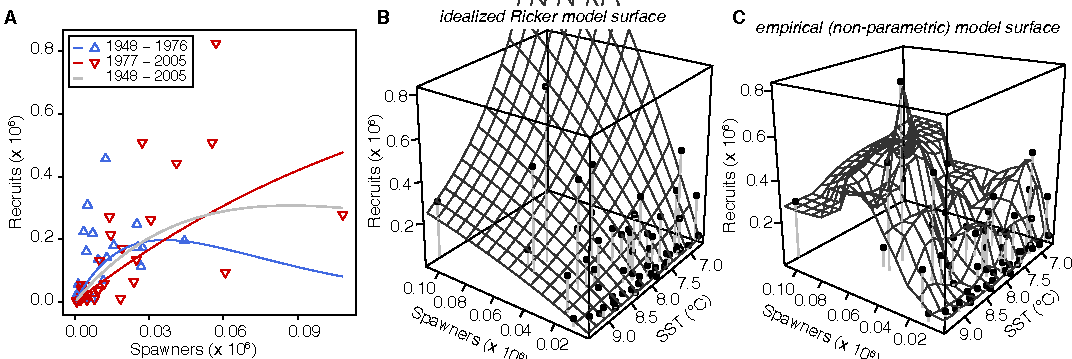
\includegraphics[width=\maxwidth{\textwidth}]{fig_salmon_1.pdf}\end{center}
\caption[Model output for the Ricker, extended Ricker, and multivariate EDM models.]{\textbf{Model output for the Ricker, extended Ricker, and multivariate EDM models.}\newline
(A) Ricker curves for the Seymour stock of Fraser River sockeye salmon are quite different for the early (blue; 1948--1976 brood years) vs. later (red; 1977--2005) time segments (triangles are observed data). Even fit to the whole time series (gray line), large errors remain. (B and C) Model output (surfaces; points are observed data) from the extended Ricker model (B) and EDM (C) using spawner abundance and Pine Island April SST to forecast recruitment of Seymour sockeye salmon. Although the Ricker model varies smoothly, it can forecast recruitment to be many times higher than the historical maximum. In the EDM model, however, the relationship between temperature and spawners is defined empirically by the data and, thus, more realistically depicted.}
\label{fig_salmon_model_surface}
\end{figure}

A common problem when applying the parametric approach to nonlinear systems is that of ephemeral fitting. That is, although population models may assume that demographic parameters such as growth rate or carrying capacity are fixed constants; these quantities are often observed to vary in time or in relation to other variables (e.g., resource availability, changing climate regimes) when tested on actual data \cite{Walters_1987}. This principle is illustrated in Figure \ref{fig_salmon_model_surface}A, where the Ricker spawner-recruit relationship is fit to the early (1948-1976) and late (1977-2005) halves of the time series from the Seymour stock. Very different relationships emerge in these two time periods, conflicting with the assumption of a fixed equilibrium and constant parameter values. Indeed, Beamish et al. \cite{Beamish_2004} found that the Ricker model fit better when constrained by climate regimes, suggesting that the spawner-recruit relationship does vary in time, a fact consistent with the general notion of nonlinear state dependence \cite{Sugihara_2012, Deyle_2013}.

At its core, nonlinear dynamics (which are known to be ubiquitous in marine species \cite{Hsieh_2005, Glaser_2014a}) occur when variables have interdependent effects; this can be problematic when applying a reductionist approach to understand nonlinear systems. For example, in laboratory experiments, guppies (\emph{Poecilia reticulatus}) preferentially eat Drosophila or tubificid worms depending on which prey is more abundant \cite{Murdoch_1975}. Thus, the strength of predation on, say, Drosophila, will change depending on the abundance of tubificid worms. This prey switching behavior typifies nonlinear state-dependence, whereby different components cannot be treated independently, as would be the case in a linear system or even a nonlinear system approximated at equilibrium. Consequently, applying a model that assumes separability of effects (e.g., vector autoregression \cite{Engle_1987}) to a system that is actually nonlinear can give the appearance of nonstationarity or stochasticity even when the underlying mechanisms are unchanged and deterministic.

Nonlinearity is also known to affect the correct identification of causal drivers--a key prerequisite for understanding and predicting system behavior.  In nonlinear systems, because interacting variables can exhibit transient (mirage) correlations that change in magnitude or sign \cite{Sugihara_2012, Deyle_2013}, the use of correlation to identify causal environmental variables can be misleading, producing both false positives (i.e., correlation does not imply causation) and false negatives (i.e., lack of correlation does not imply a lack of causation). Given the prevalence of nonlinear interactions in ecology, mirage correlations can be misleading. Indeed, a meta-analysis examining the robustness of correlations between recruitment and the environment \cite{Myers_1998} found that only 28 out of 74 initially significant correlations were upheld when subsequent data were included.

Even when causal variables are known, their inclusion into improperly formulated models can produce conflicting results. For example, with sockeye salmon in the Fraser River: although anomalous oceanic conditions experienced by juveniles are thought to be responsible for the low abundance of returning adults in 2009 \cite{Peterman_2011, Cohen_2012, Thomson_2012}, extensions of the standard Ricker model that explicitly include environmental factors surprisingly show no significant improvements in the actual forecasts \cite{Grant_2010, MacDonald_2012, Grant_2013}. A simple explanation for this apparent contradiction is that the extended Ricker model does not accurately portray the relevant interaction between the oceanic environment and sockeye salmon. Indeed, the model naively assumes that the environment acts on recruitment dynamics independently with a constant multiplicative effect (e.g., a 1$^\circ$C decrease in temperature always doubles recruitment regardless of other factors important to the state of the system). While temperature, in all likelihood, does affect recruitment, it probably does not follow this arbitrary form. We demonstrate this by fitting the model to Pine Island sea surface temperature (SST) and Seymour spawner-recruit data (Figure \ref{fig_salmon_model_surface}B), finding that the model predicts unrealistically high recruitment (much higher than the historically observed maximum) for hypothetical (but plausible) conditions of high spawner abundance and low temperature. Thus, although the equation may appear reasonable as a hypothesis, it apparently does not  incorporate the environment realistically.

\subsection{Empirical Dynamic Modeling}
In contrast to fitting an assumed set of equations, Empirical Dynamic Modeling (EDM) instead relies on time series data to reveal the dynamic relationships among variables as they occur \cite{Dixon_1999, Sugihara_2012, Sugihara_1990, Liu_2012, Glaser_2014}. By extracting these relationships empirically, EDM accommodates potentially complex and changing interactions that cannot be described in a simple set of equations. Thus, prediction accuracy with EDM is constrained by the quantity and quality of data rather than by the hypotheses represented in a set of equations (which may be subject to process error due to false or incomplete specification \cite{Sugihara_1994}).

Fundamental to EDM is the concept of a time series as an observation on a dynamic system. Broadly speaking, a dynamic system can be viewed as a set of states (d-dimensional vectors where each coordinate is a system variable) and deterministic rules (governing dynamics) for how the states evolve over time. Collectively, the set of states and their trajectories forms an ``attractor manifold'', and projecting the motion on this manifold to a coordinate axis produces a time series of the corresponding variable (Figure \ref{fig_salmon_lorenz_reconstruction}A). For example, in a simple predator-prey system where the system evolves as a function of the two abundances, the system state could be represented as the ordered pair of predator and prey abundances. This system state can be projected onto the prey coordinate axis to produce a time series of prey abundance, though many other observation functions are also possible (e.g., predator abundance, average number of prey for each predator).

In theory, with time series for all the system variables, it would be possible to reconstruct the original attractor manifold by plotting each time series as a separate coordinate. In practice, however, we typically do not have these data or know the identity of all relevant variables. Fortunately, a fundamental mathematical result proves that information about the entire system is contained in any one variable \cite{Takens_1981, Deyle_2011}, meaning that a shadow version of the original attractor can be constructed from just a single time series. This is accomplished by substituting lags of that time series for the unknown or unobserved variables (Figure \ref{fig_salmon_lorenz_reconstruction}B). These essential mechanics of EDM are detailed in \cite{Sugihara_2012} and crisply summarized in a short animation (SI Movie).

Although a single time series is usually sufficient to reconstruct a system's dynamics, there are exceptions (e.g., it is not a closed system). In the case of sockeye salmon, abundance alone may not skillfully predict future returns because they are influenced by external environmental factors. Here, the environment may be thought to act as stochastic external forcing, necessitating its inclusion as an additional coordinate in a multivariate reconstruction \cite{Dixon_1999, Deyle_2013, Deyle_2011}. We demonstrate this by using spawners and sea-surface temperature to predict recruitment (Figure \ref{fig_salmon_model_surface}C). Unlike a parametric model in which a hypothesized interaction must be specified in advance (the extended Ricker model, Figure \ref{fig_salmon_model_surface}B), the empirical surface in Figure \ref{fig_salmon_model_surface}C makes no assumptions about the relationship between variables, but instead captures the interaction between density-dependence and environmental conditions as revealed by the data: ocean temperatures have a stronger effect on recruitment when spawner abundance is low. 

\subsection{Fraser River Sockeye Salmon}

\begin{figure}[!ht]
\begin{center}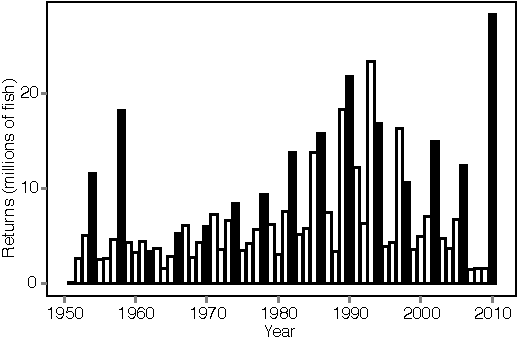
\includegraphics[width=\maxwidth{\textwidth}]{fig_salmon_2.pdf}\end{center}
\caption[Combined returns of Fraser River sockeye salmon.]{\textbf{Combined returns of Fraser River sockeye salmon.}\newline
Total returns (Dataset S1) for Fraser River sockeye salmon combined across stocks (1954 cycle line in black). Although not all stocks exhibit cyclic dominance, and those that do are not synchronized, cycles are still visible in the aggregated returns.}
\label{fig_salmon_returns}
\end{figure}

\begin{figure}[!ht]
\begin{center}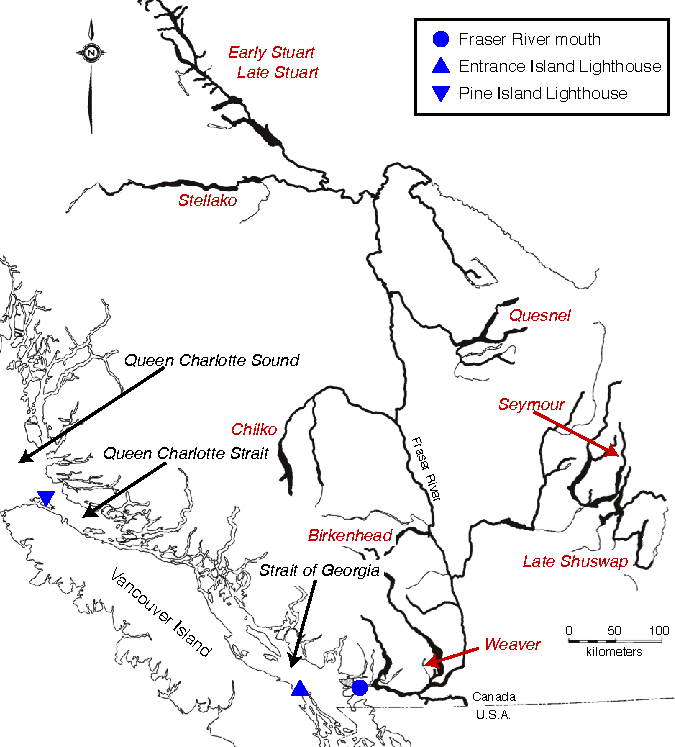
\includegraphics[width=\maxwidth{\textwidth}]{fig_salmon_3.pdf}\end{center}
\caption[Early ocean environment for Fraser River sockeye salmon.]{\textbf{Early ocean environment for Fraser River sockeye salmon.}\newline
Upon exiting the Fraser River, juvenile sockeye salmon migrate north through the Strait of Georgia, spending up to a month moving through this ecosystem \cite{Preikshot_2012}, before continuing through Queen Charlotte Strait and into Queen Charlotte Sound. Red labels for the nine stocks studied in this work are located at the approximate spawning sites. Blue triangles denote the locations of the two lighthouses where SST is recorded. Image courtesy of DFO.}
\label{fig_salmon_map}
\end{figure}

In this work, we perform a real-world test comparing EDM and the standard parametric paradigm, by forecasting returns for the 9 most historically abundant stocks of sockeye salmon from the Fraser River system in British Columbia, Canada (Figure \ref{fig_salmon_returns}), of significance to Canada's iconic fisheries. Total returns in this system are highly variable and can span over an order of magnitude: a record low of 1.6 million in 2009 was followed by a record high of 28.3 million in 2010 (Figure \ref{fig_salmon_map}). Although some of this variability occurs because of cyclic dominance \cite{Ricker_1950, Cass_1994}, large interannual fluctuations in mortality and productivity (recruits-per-spawner) are difficult to predict, leading to considerable uncertainties in current parametric forecast models \cite{Grant_2011}. This is suggestive of nonlinear dynamics in this fishery, and indeed, a Canadian federal inquiry \cite{Cohen_2012, Thomson_2012} concluded that recent declines in productivity could not be attributed to any single mechanism, but were likely caused by the interaction of multiple stressors (e.g., predators, food availability, environment). Applying a simple S-map test (p = 0.002) (\nameref{salmon_supplement}, Figure \ref{fig_salmon_nonlinearity}), we confirm the presence of nonlinear dynamics among returns of Fraser River sockeye salmon.

Thus, we apply EDM methods to unravel the mechanisms by which the environment may affect sockeye salmon recruitment. First, we compare the classical Ricker spawner-recruit model with equivalent EDM spawner-recruit models. With nearly all adults returning as age 4 or age 5 fish, we can consider the total returns in a single calendar year to be composed of age 4 and age 5 recruits from different spawning broods. Following \cite{Grant_2010}, we predict annual returns by first estimating total recruitment for each spawning brood year. This recruitment is then partitioned by age, and the age 4 and age 5 estimates from separate brood years combined appropriately to forecast returns (\nameref{salmon_materials}). Note that the time series of spawning abundance and recruitment already account for the effects of the fishery (this information is contained within the time series, see \nameref{salmon_materials}), which enables us to focus on just the natural population dynamics.

Second, to investigate the causal influence of the oceanic environment, we consider forecasts produced by the extended Ricker model and equivalent multivariate EDM formulations. In both cases, if the inclusion of environmental variables significantly improves forecasts (\nameref{salmon_materials}), those variables are taken to have a causal influence on salmon recruitment.

Lastly, to avoid arbitrary fitting and to obtain a robust measure of forecast skill, we apply a 4-fold cross-validation scheme for each model: the model is fit to $\frac{3}{4}$ of the data to predict the remaining $\frac{1}{4}$ out-of-sample, and the procedure is repeated for each $\frac{1}{4}$ segment of the time series.

\begin{figure}[!ht]
\begin{center}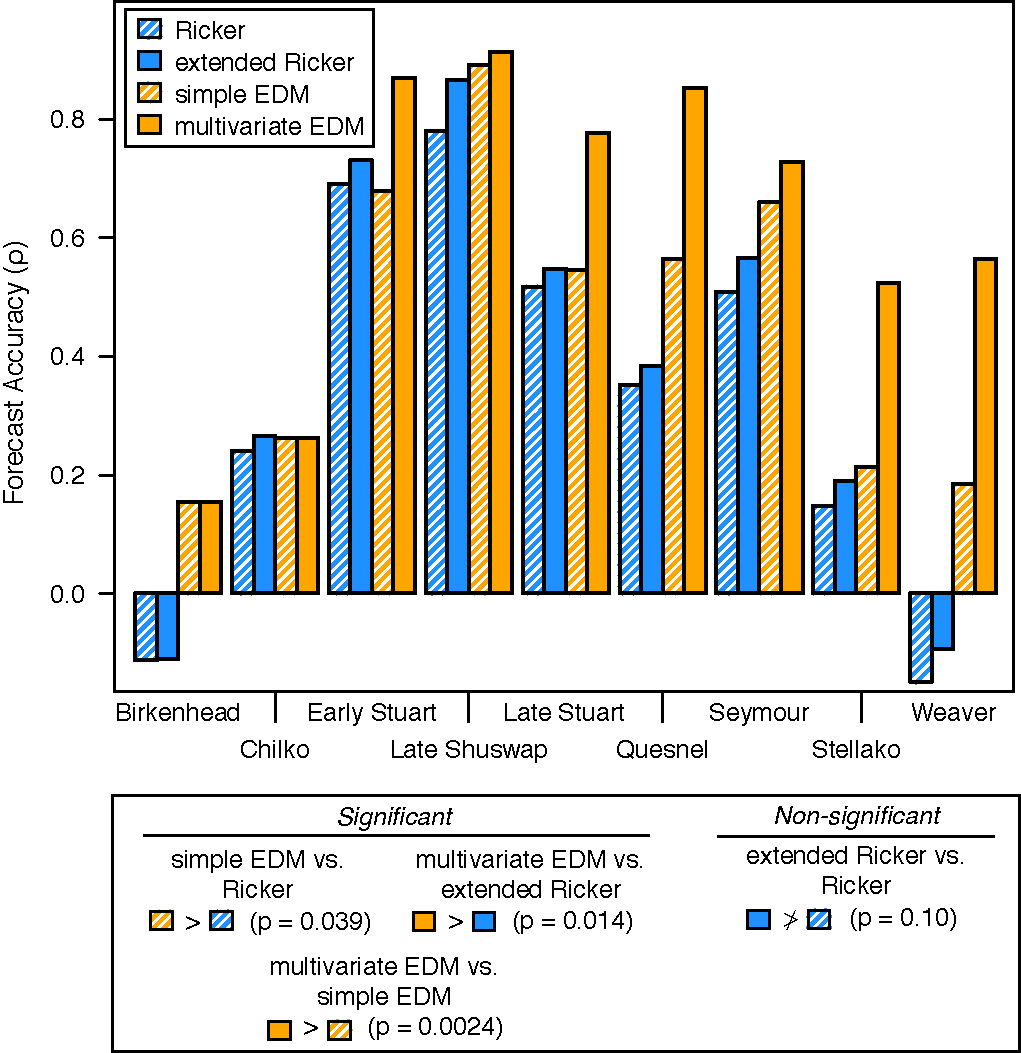
\includegraphics[width=\maxwidth{\textwidth}]{fig_salmon_4.pdf}\end{center}
\caption[Comparison of forecast accuracy.]{\textbf{Comparison of forecast accuracy.}\newline
Comparisons between equivalent EDM and Ricker models show better forecast accuracy for the EDM models [simple EDM vs. Ricker, $t_{(492)} = 1.77$, $P = 0.039$; multivariate EDM vs. extended Ricker, $t_{(492)} = 2.20$, $P = 0.014$]. Additionally, including environmental data significantly improves accuracy for EDM [$t_{(492)} = 2.83$, $P = 0.0024$], but not for the Ricker models [$t_{(492)} = 1.26$, $P = 0.10$].}
\label{fig_salmon_model_comparison}
\end{figure}

\section{Results}

\subsection{Comparison of Spawner-Recruit Forecast Models}

As a fair comparison with the standard Ricker model where spawner abundance is used to predict recruitment, we examine an equivalent EDM spawner-recruit model, but which actually has fewer fitted parameters (\nameref{salmon_materials}). Figure \ref{fig_salmon_model_comparison} shows that this simple EDM model has significantly higher accuracy ($\rho$, correlation between observations and predictions) than the Ricker model, with more accurate forecasts in 8 of 9 cases and significantly lower error overall [mean absolute error (MAE); Figure \ref{fig_salmon_model_comparison_mae}). Nonetheless, predictions for several stocks (Birkenhead, Chilko, Stellako, and Weaver) are not very skillful ($\rho < 0.3$), suggesting that in these cases, there is no simple spawner-recruit relationship (parametric or otherwise). Instead, environmental factors (e.g., sea-surface temperature, food availability) may dominate, and better performance can be obtained by accounting for these external drivers.

\subsection{Incorporating Environmental Influences}

\begin{table}
\caption[Forecast skill of models incorporating the environment]{\textbf{Forecast skill of models incorporating the environment}\newline
D, Fraser River discharge; ET, Entrance Island SST; PDO, Pacific Decadal Oscillation; PT, Pine Island SST.} \label{tab_salmon_forecast_skill}

\begin{center}
\begin{tabular}{lclcrr}
\hline
Stock & Model & Predictors & No. predictions & \multicolumn{1}{c}{$\rho$} &  \multicolumn{1}{c}{MAE} \\
\hline
Birkenhead & Ricker & $S$, $\mathrm{ET}_{\mathrm{jun}}$ & 57 & -0.111 & 0.251 \\
& EDM & $S$ & 57 & 0.156 & 0.259 \\
Chilko & Ricker & $S$, $\mathrm{ET}_{\mathrm{may}}$ & 57 & 0.268 & 0.825 \\
& EDM & $S$ & 57 & 0.264 & 0.839 \\
Early Stuart & Ricker & $S$, $\mathrm{ET}_{\mathrm{apr}}$ & 57 & 0.737 & 0.172 \\
& EDM & $S$, $\mathrm{D}_{\mathrm{apr}}$, $\mathrm{D}_{\mathrm{jun}}$ & 57 & 0.878 & 0.140 \\
Late Shuswap & Ricker & $S$, $\mathrm{ET}_{\mathrm{jun}}$ & 57 & 0.875 & 0.842 \\
& EDM & $S$, $\mathrm{D}_{\mathrm{may}}$, $\mathrm{PT}_{\mathrm{jul}}$ & 57 & 0.923 & 0.821 \\
Late Stuart & Ricker & $S$, $\mathrm{D}_{\mathrm{jun}}$ & 56 & 0.552 & 0.423 \\
& EDM & $S$, $\mathrm{D}_{\mathrm{jun}}$, $\mathrm{ET}_{\mathrm{apr}}$ & 56 & 0.783 & 0.250 \\
Quesnel & Ricker & $S$, $\mathrm{ET}_{\mathrm{jun}}$ & 57 & 0.387 & 2.057 \\
& EDM & $S$, $\mathrm{PT}_{\mathrm{may}}$, $\mathrm{PDO}$ & 57 & 0.861 & 0.729 \\
Seymour & Ricker & $S$, $\mathrm{PT}_{\mathrm{apr}}$ & 57 & 0.571 & 0.076 \\
& EDM & $S$, $\mathrm{PT}_{\mathrm{jul}}$ & 57 & 0.734 & 0.065 \\
Stellako & Ricker & $S$, $\mathrm{ET}_{\mathrm{may}}$ & 57 & 0.191 & 0.250 \\
& EDM & $S$, $\mathrm{PT}_{\mathrm{apr}}$, $\mathrm{PDO}$ & 57 & 0.531 & 0.217 \\
Weaver & Ricker & $S$, $\mathrm{PDO}$ & 39 & -0.094 & 0.215 \\
& EDM & $S$, $\mathrm{D}_{\mathrm{apr}}$, $\mathrm{D}_{\mathrm{may}}$ & 39 & 0.573 & 0.176 \\
\hline
\end{tabular}
\end{center}
\end{table}

As in the actual forecast models \cite{Grant_2010}, we further consider 3 environmental variables (the Pacific Decadal Oscillation (PDO), sea-surface temperature (SST), and Fraser River discharge) observed at different times and locations (12 time series in total). Each of these factors is believed to have a potential effect on recruitment, though significance has yet to be demonstrated in practice. For each stock, we compare the relative performance of the extended Ricker and corresponding multivariate EDM models that incorporate these environmental variables (Table \ref{tab_salmon_forecast_skill}; \nameref{salmon_materials}). Figure \ref{fig_salmon_model_comparison} shows that multivariate EDM is consistently and significantly better at forecasting than the extended Ricker model for all 9 stocks, and is true for both accuracy and precision metrics (Figure \ref{fig_salmon_model_comparison_mae}). Here, the relevant causal influence of these environmental variables is verified by the fact that multivariate EDM models that include them perform significantly better than their simple EDM spawner-recruit counterparts.

By contrast, the extended Ricker models show no significant improvement over the simple Ricker models in any of the stocks. The difference between EDM and Ricker is especially visible for Late Stuart, Quesnel, Stellako, and Weaver, indicating that these particular environmental factors (currently considered in assessments) can explain much of the variability in these stocks, provided they are incorporated reasonably (i.e., with the minimal assumptions of EDM). For Birkenhead and Chilko however, multivariate EDM models performed no better than the simplified stock-recruit versions, hinting that variables other than these are required to understand the dynamics of those stocks.

\section{Discussion}

\subsection{Nonlinearity of Fraser River Sockeye Salmon}

Similar to many marine species \cite{Hsieh_2005, Glaser_2014a}, Fraser River sockeye salmon show strong evidence for nonlinear dynamics (Figure \ref{fig_salmon_nonlinearity}, Table \ref{tab_salmon_nonlinearity}). Thus, it should not be surprising that a simple EDM model, which accommodates nonlinearity, would outperform the assumed spawner-recruit equation of the Ricker model. Furthermore, because sockeye salmon are exposed to different sources of environmentally driven mortality and because it is likely that they integrate these effects in a nonlinear fashion, it should not be surprising that multivariate EDM models that explicitly accommodate relevant environmental factors would show dramatically improved performance. In contrast, the extended Ricker model cannot resolve the nonlinear effect of the environment, and shows only non-significant improvements (that might be expected from having additional degrees of freedom).

\subsection{Identifying Environmental Drivers}

It is believed that growth during the early marine stage for Pacific salmon is a critical period that determines subsequent mortality and recruitment \cite{Beamish_2001, Beamish_2004a}. Thus, it is reasonable to expect that including related environmental variables into models should improve predictions. However, the extended Ricker model did not improve when river discharge, SST, or the PDO (Figure \ref{fig_salmon_model_comparison}, Figure \ref{fig_salmon_model_comparison_mae}) were included. Rather than suggesting that these variables have no effect, it is more likely that the extended Ricker model is incorrectly specified. This is borne out by the fact that these factors produce improved forecasts for many stocks when included non-parametrically in EDM (Figure \ref{fig_salmon_model_comparison}, Figure \ref{fig_salmon_model_comparison_mae}). Thus, our analysis suggests that the tested variables are indeed informative about the relevant environmental conditions experienced by juvenile sockeye salmon. For example, river discharge and SST may indicate primary productivity in the Strait of Georgia and other areas through which juveniles migrate (Figure \ref{fig_salmon_returns}) \cite{Thomson_2012, Beamish_1994, Preikshot_2012}, and the associations between large-scale oceanic climate indicators such as the PDO and Pacific salmon productivity are well-known from other studies \cite{Mantua_1997, Beamish_1997}. While these variables do not reflect direct causal mechanisms, they may be useful as simple indicators of processes that influence salmon survival, thereby improving forecasts when included in the EDM approach.

While individual stocks appear to be sensitive to different environmental factors (Table \ref{tab_salmon_forecast_skill}), we did observe some general patterns: for example, 2 of the 9 stocks (Stellako and Quesnel) identified the PDO as an informative variable (the first-ranked EDM models for these stocks include the PDO as a coordinate), yet the predictability for these stocks is further improved when other variables (river discharge or SST) are included in addition to the PDO. This suggests that the PDO is an incomplete observation on the relevant environment for sockeye, and that local-scale measures of the environment can enhance the information in the PDO index (an ocean basin-scale indicator) (see \nameref{salmon_supplement} for details).

Although our models confirm a general influence of the environment on sockeye salmon recruitment, some stocks appear to be skillfully predicted using only spawner abundance. One explanation for this is that the stocks experience unique environments: they are exposed to different freshwater conditions in their respective nursery lakes, and they exhibit different timings and migration routes as they travel through the Fraser River (T. Whitehouse, DFO, pers. comm.), the Strait of Georgia \cite{Beacham_2014}, and along the west coast of North America \cite{Tucker_2009}. Even with shared environmental influences (e.g., food availability in the Strait of Georgia), nonlinear state-dependence can produce dynamics unique to each stock. Consequently, if these myriad effects are strongly density-dependent, recruitment could be successfully predicted using just spawner abundance. However, if these effects are stochastic (i.e., environmentally-driven), then it will be necessary to include informative indicator variables to improve forecasts.

Apart from multivariate models, an alternative approach to determine causal environmental variables would be to apply the method of convergent cross mapping (CCM, \cite{Sugihara_2012}). However, due to data limitations (in particular, the absence of annual monitoring of each cycle line including the oceanic phase), CCM may not be sufficiently sensitive to resolve causality here (see \nameref{salmon_supplement} for details)

\subsection{Nonuniqueness of Models}

We note that, for a given stock, different EDM models can show similar performance (Table \ref{tab_salmon_multivariate_full}). Although somewhat counter-intuitive, this phenomenon is expected, because the tested variables (river discharge, SST, the PDO) are proxy indicators of the environment. Thus, they may contain redundant information such that different variable combinations are equally informative even as they represent alternative perspectives on the system. This reflects a fundamental property of EDM in that forecast performance depends solely on the information content of the data rather than on how well assumed equations match reality.

To clarify the concept of non-uniqueness, consider the canonical Lorenz attractor (Figure \ref{fig_salmon_lorenz_reconstruction}A). The behavior of this system is governed by three differential equations (Equation \ref{eqn_lorenz}). However, the axes can be rotated to produce 3 new coordinates, $x^\prime$, $y^\prime$, and $z^\prime$ and the equations rewritten in terms of these new coordinates, allowing the system to be described using either representation ($x$, $y$, and $z$ OR $x^\prime$, $y^\prime$, and $z^\prime$) as well as mixed combinations (e.g., $x$, $y$, and $z^\prime$). Thus, with an infinite number of ways to rotate the system, there are an unlimited number of ``true variables'' and ``true models.'' In the case of sockeye salmon, the similar performance of different models (Table \ref{tab_salmon_multivariate_full}) does not mean that one or the other model is incorrect; instead, it reflects the fact that the environmental variables are indicators of the same general mechanism, and so different variable combinations can be equally informative for forecasting recruitment.

Again, we emphasize that including a variable does not imply a direct causal link -- variables in an EDM model improve forecasts because they are informative; it does not mean that the included variables are proximate causes. Importantly, the converse does not hold either: a variable could be causal and yet not appear in the multivariate EDM; this might occur when multiple stochastic drivers affect recruitment in an interdependent way, necessitating that a model include measurements of all the drivers to account for their combined effect. For example, although none of the tested variables seem to improve forecasts for the Birkenhead stock (Table \ref{tab_salmon_multivariate_full}), this does not mean that these sockeye salmon are insensitive to SST, river discharge, and the PDO. Rather, it suggests that the effect of these variables may be modulated by other factors not considered here.

\subsection{Data Requirements of EDM}

Using EDM is fundamentally a data-driven approach: thus, it is important to ensure that time series are of sufficient length to recover dynamics. For example, Sugihara et al. \cite{Sugihara_2012} suggest that at least 35-40 points might be necessary as a rough minimum, though methods exist for using dynamically similar replicates in cases where time series are shorter \cite{Hsieh_2008}. For many systems, however, the data requirements of EDM mean that increased budgets and additional sampling effort will be important to support long-term continuous observations and generate sufficient time series. We note, though, that it is not necessary to sample all putatively relevant drivers, because different measurements are often substitutable as proxies for true proximal causes.

When data requirements are met, however, we note that collecting additional data can further improve accuracy and precision of EDM models. Consider the simplex projection method, which uses nearest-neighbor analogues to approximate system behavior. With each new data point, more analogues are available (the reconstructed manifold becomes denser), and so these approximations become more precise. Thus, EDM models will improve with longer time series. In contrast, a parametric model will benefit from more data only when the assumed equations are essentially correct. In the case of the classic Ricker model in Figure \ref{fig_salmon_model_surface}A, it is clear that similar levels of spawner abundance yield very different levels of recruitment, and so any simple function relating the two cannot fully explain the scattered observations. Adding more data may result in more ``precise'' parameter estimates, but individual errors will remain large when the underlying process is more complex than the assumed model can portray.

\subsection{Alternative Parametric Models}

In this work, we use the classical and extended Ricker models as examples of the parametric approach, but acknowledge that there are alternative models considered by the DFO for Fraser River sockeye salmon \cite{Peterman_2000, Haeseker_2007, Haeseker_2008, Grant_2012}. While some of these models may fit the data better, this does not always reflect a model's true performance in out-of-sample forecasting. For example, a modified Ricker model that allows parameters to randomly drift over time \cite{Peterman_2000} will explain variations in the data better than the static alternative, because doing so can indirectly track nonlinear state-dependence. However, instead of a mechanism for why parameters change, such models based on the Kalman filter \cite{Kalman_1960} typically use forward information (i.e., observations at time $t+1$ help to estimate the growth rate at time $t$), and thus do not actually ``predict.'' Consequently the actual forecast performance of such models will be overestimated by their fit to historical data. A more fundamental concern with the parametric approach is that it requires explicit equations to model the effects of included variables. Such equations may be overly simplified (e.g., linear correlations) and unable to accommodate the state-dependent effects that occur in nonlinear systems.

\subsection{Final Remarks}

EDM addresses two important challenges for modeling natural systems. First, EDM identifies relevant variables and interactions empirically and dynamically \cite{Sugihara_2012}; this is in contrast to the conventional approach where the use of parametric equations poses the dual risks of model misspecification \cite{Sugihara_1994} as well as variable misidentification \cite{Sugihara_2012, Deyle_2013, Myers_1998}. Importantly, EDM allows proxy variables to be used, which can be a boon when observations on key processes (e.g., mortality) are lacking but indirect measurements (e.g., SST) are available. Second, the equation-free approach of EDM produces more accurate forecasts than equivalent parametric models using the same data. As Perretti et al. \cite{Perretti_2013} have shown, even when a correct parametric model is known, fitting parametric models can be problematic, and is an important concern with many systems exhibiting nonlinear behavior \cite{Hsieh_2005, Glaser_2014a}. In contrast, EDM models can capture dynamic information and explain behavior that may be misclassified as random by parametric fitting procedures.

Consequently, the dynamic perspective of EDM has much to offer for modeling nonlinear systems, representing a viable framework (with minimal assumptions) for system identification and robust forecasting. When parametric models are required, EDM can also be used in a complementary role to identify causal links, recover variable relationships, and even guide the construction of reliable equation-based models \cite{Crutchfield_1987}. This represents a practical way to perform data-driven modeling instead of starting with complex parametric models (end-to-end ecosystem models, such as Ecopath with Ecosim \cite{Christensen_2004}), which often make strong assumptions and require large amounts of data to parameterize.

Moreover, EDM models can also serve as direct substitutes for their parametric equivalents. Here, our simple and multivariate EDM models are formulated similarly to their Ricker-based counterparts: using spawner abundance (and the environment) to forecast returns. Some simple extensions to the methods, such as the development of uncertainty estimates (see \nameref{salmon_supplement}, Figure \ref{fig_salmon_standard_error}), will enable these models to be integrated into the current management framework that uses parametric models. Thus, we believe that EDM has great potential as a tool for understanding and forecasting nonlinear ecosystems: by operating without assumed equations, it can be beneficial when exact mathematical descriptions are not available.

\section{Materials and Methods}
\label{salmon_materials}

\subsection{Data}

We analyze yearly time series data for the 9 historically most abundant stocks (Birkenhead, Chilko, Early Stuart, Late Shuswap, Late Stuart, Quesnel, Seymour, Stellako, and Weaver) of sockeye salmon from the Fraser River system. Data span brood years 1948--2005, except for Late Stuart and Weaver, where data begin in 1949 and 1966, respectively. We consider only single-stock models, so notation and equations are given as for a single stock.

$S_t$ is the number of effective female spawners in brood year $t$, and $R_t$ is the corresponding recruitment (returning adults). Recruitment is partitioned by age: $R_{a, t}$  is the number spawned in year $t$ and returning at age $a$ in year $t + a$. Following \cite{Grant_2010}, total recruitment is the sum of age 4 and age 5 recruits: $R_t = R_{4, t} + R_{5, t}$. In contrast, total returns, $N_y$, are the adults that return to spawn in calendar year $y$, and computed as $N_y = R_{4, y-4} + R_{5, y-5}$. As explained below, recruitment is forecast from spawner abundance, and age 4 and age 5 recruits (from different brood years) are summed to estimate total returns in a given calendar year. Note that both recruitment and returns are computed as catch + escapement + en-route loss, while spawner abundance is based on observations of escapement and egg production \cite{Grant_2011}. Thus, both spawner abundance and recruitment account for the effects of catch, and the models we consider here focus just on the population dynamics of this system.

We investigate 3 environmental variables: the Pacific Decadal Oscillation (PDO), sea-surface temperature (SST), and Fraser River discharge. For the PDO, one annual time series is constructed as the average of monthly values from November to March \cite{Mantua_1997}. SST measures are monthly averages from two lighthouse stations (Entrance Island: April to June and Pine Island: April to July). River discharge is measured at Hope; we include peak daily flow and monthly averages (April to June). Fraser River sockeye salmon enter the ocean at age 2, so the environmental data are lagged 2 years to line up with ocean entry time.

\subsection{Attractor Reconstruction}

The goal of attractor reconstruction is to approximate the originating dynamic system using time series data. The simplest construction uses successive lags of a single time series \cite{Takens_1981, Packard_1980}: given time series $\{x_t\}$, $E$-dimensional vectors $\vec{x}_t$ are composed of $E$ lags of $x$, each separated by a time step $\tau$: $\vec{x}_t = \langle x_t, x_{t-\tau}, \dots x_{t-(E-1)\tau}\rangle$.

Generalizations of Takens' theorem \cite{Deyle_2011, Sauer_1991} permit attractor reconstructions using multiple time series. For example, with $\{x_t\}$ and $\{y_t\}$ observed from the same system, one possible reconstruction forms vectors as $\langle x_t, y_t, y_{t-\tau}\rangle$. To account for different scaling between variables, each time series is first linearly transformed to have mean $= 0$ and variance $= 1$.

\subsection{Simplex Projection and S-map}

Simplex projection estimates the trajectory (i.e., forecasts) of a novel system state by computing a weighted average of the trajectories of that state's nearest neighbors \cite{Sugihara_1990}. Given an attractor reconstruction, and a novel state $\vec{x}_s$, we first find the $b$ nearest neighbors (typically setting $b = E + 1$) that are closest to $\vec{x}_s$: these neighbors are the vectors $\vec{x}_{n(s, i)}$ where $n(s, i)$ designates the time index of the $i$th closest neighbor to $\vec{x}_s$. So, $\vec{x}_{n(s, 1)}$ is the closest neighbor to $\vec{x}_s$, $\vec{x}_{n(s, 2)}$ is the second closest neighbor, etc. We then evolve the neighbors forward, and compute a weighted average of the forward evolutions ($h$ time steps into the future) to estimate $\vec{x}_{s+h}$:

\begin{equation}
\label{eqn_simplex}
\hat{\vec{x}}_{s+h}=\left(\sum_{i=1}^{b}{w_i\left(s\right)\vec{x}_{n(s, i)+h}}\right) \bigg/ \sum_{i=1}^{b}{w_i\left(s\right)}.
\end{equation}

The weights, $w_i(s)$, are based on the distance between $\vec{x}_s$ and its $i$th neighbor, $\vec{x}_{n(s, i)}$, scaled to the distance to the nearest neighbor: \\$w_i(s) = exp\left(-d(\vec{x}_s, \vec{x}_{n(s, i)})/d(\vec{x}_s, \vec{x}_{n(s, 1)})\right)$ and $d(\vec{x}_s, \vec{x}_t)$ is the Euclidean distance between the vectors $\vec{x}_s$ and $\vec{x}_t$.

In most cases, we desire forecasts of a scalar value rather than of the full system state. This is possible when the variable to be forecast, $y$, is an observation on the same dynamic system. As such, there will be a correspondence between $\vec{x}_t$ and the scalar value of $y_t$, and we can adjust equation \ref{eqn_simplex} to compute a weighted average of the corresponding values of $y$:

\begin{equation}
\label{eqn_simplex_scalar}
\hat{y}_{s+h} = \left(\sum_{i=1}^{b}{w_i\left(s\right)y_{n(s, i)+h}}\right) \bigg/ \sum_{i=1}^{b}{w_i\left(s\right)}.
\end{equation}

The S-map procedure computes a local linear map between lagged-coordinate vectors and a target variable and is often used to test for nonlinear state-dependence \cite{Sugihara_1994}. It includes a tuning parameter, $\theta$, that controls the weights associated with individual vectors: $\theta = 0$ reduces the S-map to a linear autoregressive model of order $E$, while $\theta > 0$ gives more weight to nearby states when computing the local linear map, thus allowing for nonlinear behavior. Following \cite{Glaser_2014a, Hsieh_2006}, we test for nonlinearity by computing the decrease in forecast error (MAE) as $\theta$ is tuned to be greater than 0 (see \nameref{salmon_supplement} for details).

\subsection{Model Descriptions}

We formulate EDM models to forecast recruitment from spawner abundance, combining age 4 and age 5 recruits (from different brood years) to estimate total returns in a given calendar year. Acknowledging the persistent 4-year quasicycle, the time series of recruits and spawners are scaled so that each cycle line has mean 0 and variance 1: $S^\prime_t = \left(S_t - \mu_k(S)\right)/\sigma_k(S)$ and $R^\prime_t = \left(R_t - \mu_k(R)\right)/\sigma_k(R)$, where $k = 1, 2, 3, \mathrm{or } 4$, depending on cycle line and can be computed as $k = 1 + ((t-1) \bmod 4)$. $\mu_k$ and $\sigma_k$ are the mean and standard deviation, respectively, for the $k$th cycle line.

The simple EDM model approximates the system state with 1 lag of the transformed spawner abundance:
\begin{equation}
\vec{x}_t = \langle S^\prime_t \rangle.
\end{equation}

Forecasts of the age 4 and age 5 recruits, $R^\prime_{4, t}$ and $R^\prime_{5, t}$, are made using simplex projection. Here, the two nearest neighbors of $S^\prime_t$ are identified, and the corresponding values of $R^\prime_{4, t}$ (or $R^\prime_{5, t}$) are combined in a weighted average to produce a forecast. These forecasts are transformed back into raw values, $\hat{R}_{a, t} = \hat{R}^\prime_{a, t} \cdot \sigma_k(R_a) + \mu_k(R_a)$, and age 4 and age 5 recruits are combined to produce a forecast of total returns, $\hat{N}_y = \hat{R}_{4, y-4} + \hat{R}_{5, y-5}$.

The multivariate models combine spawner data with up to 2 environmental indicators:
\begin{align}
\begin{split}
\vec{x}_t &= \langle S^\prime_t, U^\prime_{t+2} \rangle\\
\vec{x}_t &= \langle S^\prime_t, U^\prime_{t+2}, U^{\prime\prime}_{t+2} \rangle,
\end{split}
\end{align}

where $U^\prime_{t+2}$ (or $U^{\prime\prime}_{t+2}$) is one of the environmental time series described previously, normalized to have mean $= 0$ and variance $= 1$. Just as in the simple EDM model, forecasts of the age 4 and age 5 recruits are made using simplex projection and combined to produce a forecast of total returns. However, because including environmental variables increases the embedding dimension, three nearest neighbors are used for models that include one environmental coordinate, and four nearest neighbors for models that include two environmental coordinates.

Following \cite{Grant_2010}, we use the standard Ricker model to estimate total recruitment and then partition it into age 4 and age 5 fish. age 4 and age 5 fish from separate brood years are combined to forecast the number of returns:
\begin{align}
\begin{split}
\hat{R}_t &= S_t \exp{(\alpha - \beta S_t)},\\
\hat{N}_y &= \hat{R}_{y-4} \cdot p_4 + \hat{R}_{y-5} \cdot (1 - p_4),
\end{split}
\end{align}

where $p_4$ is the average fraction of recruits that return as age 4 fish. The extended Ricker model is similar, but includes an additional term in the exponent for an environmental covariate:

\begin{equation}
\hat{R}_t = S_t \exp{(\alpha - \beta S_t + \gamma U_{t+2})}.
\end{equation}

\subsection{Fitting Procedure and Performance Measures}

To avoid testing all combinations of (and overfitting) the environmental variables in the EDM model, we sequentially add the environmental variable that most improves forecast accuracy ($\rho$, the correlation between observed and predicted values). If none of the variables improve forecasts when added, then no further environmental variables are included. Thus the best EDM model for some stocks may have only 0 or 1 environmental variable (Table \ref{tab_salmon_forecast_skill}). Similarly, for the extended Ricker model, we choose the environmental variable that gives the highest $\rho$.

The Ricker models were fit using R 3.0.2 (\url{http://www.r-project.org/}), the Rjags package (\url{http://cran.r-project.org/web/packages/rjags/index.html}), and \linebreak JAGS 3.2.0 (Just Another Gibbs Sampler; \url{http://mcmc-jags.sourceforge.net/}) following the procedure outlined in \cite{Grant_2010}. Medians of the posterior distribution are used to obtain point estimates suitable for comparison. The EDM models were constructed using R 3.0.2 and the rEDM package (\url{https://github.com/ha0ye/rEDM}). The package can be installed with the following lines of R code:
\begin{verbatim}
library(devtools)
install_github("ha0ye/rEDM")
\end{verbatim}
R scripts for the models and data files can be found in the supplementary information.

All forecasts are made using a 4-fold cross-validation procedure. To quantify model performance, we use Pearson's correlation coefficient ($\rho$) between observed and predicted returns as a measure of accuracy and MAE as a measure of error. Comparisons of $\rho$ between models uses a one-sided $t$ test with SE calculated using the HC4 estimator from \cite{Cribari-Neto_2004} and with adjusted degrees of freedom as suggested by \cite{Wilcox_2009}. Improvement in MAE is computed using a one-sided paired $t$ test for the difference, treating each forecast as an independent sample. To compute an aggregate statistic combining all 9 stocks, we first scale the observations and predictions for each stock so that the observed returns have mean $= 0$, variance $= 1$, and then combine the normalized values across stocks. The comparisons of $\rho$ and MAE are done using this combined set of observations and predictions (Figure \ref{fig_salmon_model_comparison}, Figure \ref{fig_salmon_model_comparison_mae}).

\section{Supplementary Information}
\label{salmon_supplement}

\begin{figure}[!ht]
\begin{center}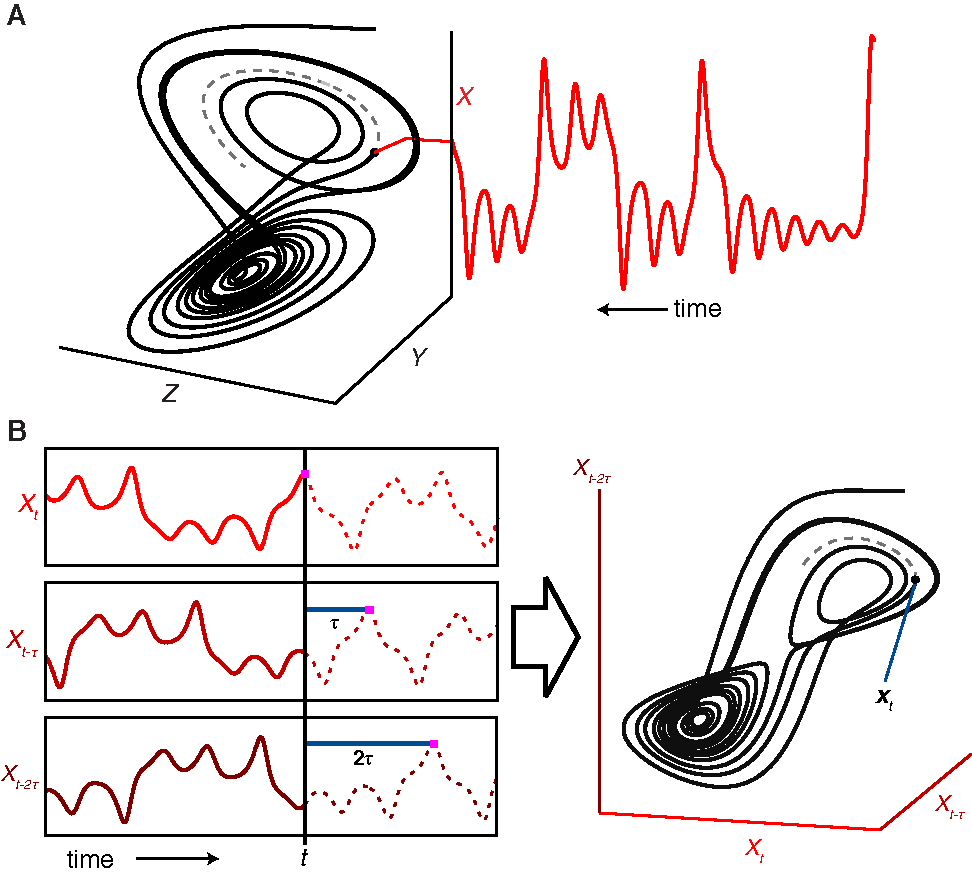
\includegraphics[width=\maxwidth{\textwidth}]{fig_salmon_s1.pdf}\end{center}
\caption[Reconstruction of system dynamics from a time series.]{\textbf{Reconstruction of system dynamics from a time series.}\newline
(A) Projecting the motion of the canonical Lorenz attractor onto the $x$-axis yields a time series for variable $x$. (B) Successive lags (with time step $\tau$) of the time series $x_t$ are plotted as separate coordinates to form a reconstructed ``shadow'' manifold that preserves essential mathematical properties of the original system (and is visually similar).}
\label{fig_salmon_lorenz_reconstruction}
\end{figure}

\subsection{Attractor Reconstruction from Time Series}

Broadly speaking, dynamic systems can be described as a set of states (i.e. a manifold) and rules (governing dynamics or hidden equations) for how the states evolve over time. Motion on the manifold can be projected onto a coordinate axis, forming a time series (Figure \ref{fig_salmon_lorenz_reconstruction}A). More generally, however, any set of sequential observations of the system state (i.e., a function that maps the state onto the real number line) is a time series.

For example, the Lorenz attractor (a simplified description of turbulent flow in the atmosphere \cite{Lorenz_1963}) is a dynamic system where the states are 3-dimensional vectors with coordinates $x$, $y$, and $z$, and whose motion is governed by three differential equations (Equation \ref{eqn_lorenz}).

\begin{align}
\label{eqn_lorenz}
\begin{split}
\frac{dy}{dt} &= 10(y-x)\\
\frac{dy}{dt} &= x(28-z)-y\\
\frac{dz}{dt} &= xy - \frac{8}{3}z
\end{split}
\end{align}

In an ecological setting, these variables could represent the abundances of different species (e.g., salmon, zooplankton, and phytoplankton), with the equations capturing the biological processes of growth, death, and predation. The projection of the system state onto one of the axes gives a time series for the population corresponding to that variable (Figure \ref{fig_salmon_lorenz_reconstruction}A).

If one knew all the relevant variables of a system, their time series could be used to reconstruct the original manifold, by plotting each variable as a separate coordinate. Given time series of sufficient length, it might even be possible to derive the equations of motion for that system. However, in nature, the system may be highly complex (hundreds or thousands of interacting variables or components), and time series are generally short. The method of time-delay embedding \cite{Takens_1981, Crutchfield_1987} offers a solution to this problem; reconstructions of a dynamic system can be made using successive lags of a single time series (Figure \ref{fig_salmon_lorenz_reconstruction}B). Takens' theorem \cite{Takens_1981} states that, if enough lags are taken, this form of reconstruction is generically a diffeomorphism and preserves essential mathematical properties of the original system. In other words, local neighborhoods (and their trajectories) in the reconstruction map to local neighborhoods (and their trajectories) of the original system. This also permits forecasting, by finding nearest neighbors from among the historical record and using their behavior to estimate how the system will evolve through time (e.g., simplex projection, see \nameref{salmon_materials}).

\begin{figure}[!ht]
\begin{center}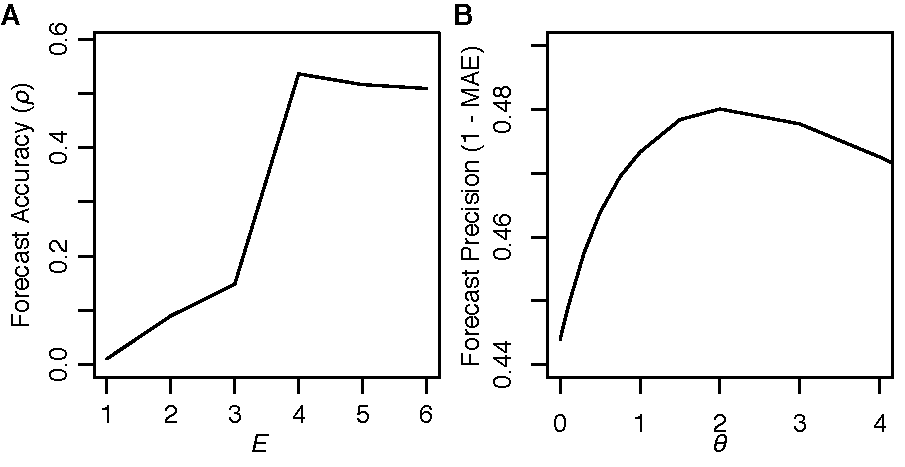
\includegraphics[width=\maxwidth{\textwidth}]{fig_salmon_s2.pdf}\end{center}
\caption[Nonlinearity in Fraser River sockeye salmon.]{\textbf{Nonlinearity in Fraser River sockeye salmon.}\newline
Following \cite{Hsieh_2008}, we concatenate time series of returns for 9 stocks. (A) Forecasting returns using simplex projection, 4 is identified as the optimal embedding dimension. (B) Using the S-map procedure, forecast skill is highest for $\theta \sim 2$ ($P = 0.002$), which demonstrates nonlinear state dependence in salmon dynamics.}
\label{fig_salmon_nonlinearity}
\end{figure}

\begin{table}
\caption[Nonlinearity tests for individual stocks.]{\textbf{Nonlinearity tests for individual stocks.}\newline
$E$ is embedding dimension, $\theta$ is the optimal value of the nonlinear tuning parameter, $\Delta$MAE is the difference in error between the model at the optimal value of $\theta$ and the model at $\theta = 0$ (negative values indicate a decrease in error, or improvement with $\theta > 0$), $P$ value is for a randomization test with 500 iterations (* indicates significance at the $\alpha = 0.10$ level).}
\label{tab_salmon_nonlinearity}

\begin{center}
\begin{tabular}{lrrrrr}
\hline
stock & $E$ & $\theta$ & $\Delta$MAE & $P$ value & significantly nonlinear? \\
\hline
Birkenhead & 5 & 0 & 0 & 0.494 & no \\
Chilko & 6 & 2 & -0.070 & *0.024 & yes \\
Early Stuart & 6 & 4 & -0.023 & *0.050 & yes \\
Late Shuswap & 4 & 2 & -0.389 & *0.014 & yes \\
Late Stuart & 8 & 3 & -0.054 & *0.060 & yes \\
Quesnel & 7 & 4 & -0.298 & *0.008 & yes \\
Seymour & 8 & 0.5 & -0.002 & 0.162 & no \\
Stellako & 7 & 2 & -0.025 & *0.014 & yes \\
Weaver & 1 & 0 & 0 & 0.496 & no \\
\hline
\end{tabular}
\end{center}
\end{table}

\subsection{Identifying nonlinearity in sockeye salmon dynamics}

One application of EDM is to identify nonlinear dynamics in time series. For the Fraser River system, we first consider the 9 stocks in aggregate. Following \cite{Hsieh_2008}, each time series of returns is linearly transformed to have mean $= 0$ and variance $= 1$. This preserves the quasicyclic behavior of each stock, but corrects for the relative magnitude across different stocks. The normalized time series are joined together end-to-end, in effect treating them as 9 instances of a single time series. Using simplex projection with $\tau = 1$ and predicting 1 year into the future, forecast skill ($\rho$) is maximized when 4 successive lags are used (Figure \ref{fig_salmon_nonlinearity}A). This is somewhat expected, because the quasicyclic nature of these returns has a 4-year periodicity: knowing the previous 4 years is sufficient to identify the current phase and estimate the current magnitude of returns.

Next, we employ the S-map procedure \cite{Sugihara_1994}, which compares equivalent linear and nonlinear models (adjusting a tuning parameter, $\theta$) to test for nonlinear dynamics. When $\theta = 0$, all points are weighted equally, and the model reduces to an autoregressive model of order $E$. For $\theta > 0$, nearby points are given stronger weighting, allowing the model to be adaptive to local influences and therefore, nonlinear. If the behavior of sockeye returns is purely periodic, then the linear model should have the highest forecast skill, because it can smooth out errors over the entire data set. However, Figure \ref{fig_salmon_nonlinearity}B shows that forecast skill peaks when $\theta$ is ~ 2, which is evidence for nonlinearity in the aggregate time series. Using the randomization test of \cite{Hsieh_2006, Glaser_2014a}, this improvement in forecast skill (decrease in MAE) is significant with $P = 0.002$.

As noted in \cite{Hsieh_2008}, nonlinearity may appear as an artifact when aggregating linear time series with somewhat different dynamics. Therefore, to confirm the presence of nonlinearity, we also apply the S-map to each stock individually, using the same randomization test for whether the improvement in forecast error (MAE) is significant at the $\alpha = 0.10$ level (Table \ref{tab_salmon_nonlinearity}). Overall, these results are encouraging: we find 6 of the 9 stocks to be significantly nonlinear. We note, however, that the lack of significant nonlinearity in the Birkenhead, Seymour, and Weaver stocks may not necessarily indicate that these stocks are linear, as the S-map test can require lengthy time series for accurate discrimination.
	
\subsection{Convergent Cross Mapping}

\begin{sidewaystable}
\caption[Results of cross mapping]{\textbf{Results of cross mapping}\newline
N is the number of predictions, 95\% $\rho$ is the critical value for significance at the $\alpha = 0.05$ level, ``xmap \{VAR\}'' columns are the cross mapping correlations for \{VAR\}, where ET is Entrance Island SST, PT is Pine Island SST, D is Fraser River discharge, and PDO is Pacific Decadal Oscillation. Highlighted cells indicate significant cross mapping at the $\alpha = 0.05$ level.}
\label{tab_salmon_ccm}

\begin{center}
\resizebox{8.8in}{!}{
\begin{tabular}{l|rr|rrrr|rrr|rrrr|r}
\hline
stock & N & 95\% $\rho$ & \specialcellR{xmap\\D$_\mathrm{max}$} & \specialcellR{xmap\\D$_\mathrm{apr}$} & \specialcellR{xmap\\D$_\mathrm{may}$} & \specialcellR{xmap\\D$_\mathrm{jun}$} & \specialcellR{xmap\\ET$_\mathrm{apr}$} & \specialcellR{xmap\\ET$_\mathrm{may}$} & \specialcellR{xmap\\ET$_\mathrm{jun}$} & \specialcellR{xmap\\PT$_\mathrm{apr}$} & \specialcellR{xmap\\PT$_\mathrm{may}$} & \specialcellR{xmap\\PT$_\mathrm{jun}$} & \specialcellR{xmap\\PT$_\mathrm{jul}$} & \specialcellR{xmap\\PDO} \\
\hline
Birkenhead & 58 & 0.218 & 0.108 & -0.294 & 0.105 & 0.182 & 0.141 & -0.122 & 0.046 & -0.13 & -0.003 & 0.029 & -0.024 & -0.151 \\
Chilko & 58 & 0.218 & -0.197 & 0.045 & 0.172 & -0.085 & 0.161 & -0.024 & 0.215 & 0.244 & 0.194 & 0.288 & 0.211 & 0.042 \\
Early Stuart & 58 & 0.218 & -0.005 & -0.015 & 0.166 & 0.054 & 0.468 & 0.459 & 0.107 & 0.276 & 0.300 & 0.275 & 0.255 & -0.079 \\
Late Shuswap & 58 & 0.218 & -0.300 & 0.034 & -0.178 & -0.178 & -0.081 & 0.309 & 0.011 & 0.024 & 0.018 & 0.166 & 0.199 & 0.192 \\
Late Stuart & 57 & 0.220 & 0.007 & 0.036 & -0.058 & -0.023 & 0.481 & 0.512 & 0.442 & 0.313 & 0.377 & 0.313 & 0.242 & 0.182 \\
Quesnel & 58 & 0.218 & 0.107 & 0.443 & -0.033 & 0.087 & 0.599 & 0.371 & 0.243 & 0.523 & 0.611 & 0.562 & 0.532 & 0.200 \\
Seymour & 58 & 0.218 & -0.326 & 0.006 & 0.157 & -0.212 & 0.057 & -0.185 & -0.279 & 0.093 & -0.073 & 0.069 & 0.219 & 0.230 \\
Stellako & 58 & 0.218 & -0.326 & 0.006 & 0.157 & -0.212 & 0.057 & -0.185 & -0.279 & 0.093 & -0.073 & 0.069 & 0.219 & 0.230 \\
Weaver & 40 & 0.264 & -0.076 & 0.122 & -0.285 & 0.044 & -0.116 & -0.213 & -0.067 & -0.286 & -0.085 & -0.068 & 0.043 & -0.125 \\ 
\hline
\end{tabular}
}
\end{center}
\end{sidewaystable}

If salmon mortality is strongly influenced by the environment, then the time series of salmon recruitment will contain information about past environmental states. This means that it is possible to estimate past environmental conditions from salmon abundances. To the extent that this is true, the ability to recover past environmental states from the salmon time series is evidence for causal influence by the environment. This criterion for causation (convergent cross mapping, CCM) can be used to identify key variables and operates in nonlinear systems whereas linear correlation does not \cite{Sugihara_2012, Deyle_2013}.

CCM operates on much the same principle as generalized simplex projection in Equation \ref{eqn_simplex_scalar} (see \nameref{salmon_materials} in main text). Here, the notion is that if variable $y$ has a causal influence on $x$, then the system state (represented using only lags of $x$) will contain an imprint of $y$. Thus, it should be possible to map between states of the system (the univariate reconstruction based on $x$) and the value of $y$. Cross mapping strength can be assessed by the correlation between the estimated values of y and the corresponding observed values. In a fully deterministic system with no noise, we expect this cross mapping correlation to approach 1 as time series length increases and the reconstruction becomes denser. As a practical indicator of causal influence, here we test whether the correlation is significantly positive when using the whole time series.

It is important to note that if a variable $y$ is stochastic and influences $x$ with a time lag, then cross mapping from $x$ to $y$ may show evidence of a causal interaction only if the appropriately lagged value of $y$ is estimated. Here, we are interested in testing for the influence of the environment on juvenile salmon, which occurs when the salmon are 2 years old. Thus, a reconstruction based on salmon abundance for brood year $t$ should be informative about the environment in calendar year $t+2$. Moreover, because it is only the 2-year old salmon that are affected by this early oceanic environment, it would not make sense to include measures of salmon abundance from multiple spawning broods (i.e., only salmon from brood year t should have information about the environment in year $t+2$). Therefore, we use multivariate CCM, cross mapping from the reconstruction $\vec{x}_t = \langle S_t^\prime, R_t^\prime \rangle$ (where $S_t^\prime$ and $R_t^\prime$ are the cycle-line normalized spawner and recruit abundances of brood year $t$, respectively, to account for the effect of cyclic dominance) to $y_t = U_{t+2}$ (where $U_{t+2}$ is an environmental variable measured in calendar year $t+2$), to estimate the environmental effect that would have influenced that brood of salmon.

Table \ref{tab_salmon_ccm} shows the cross mapping results for each combination of the 9 stocks and 12 environmental time series considered in this work. Only some of the relationships appear significant, with most of the significant cross mapping occurring between temperature and the Chilko, Early Stuart, Late Stuart, and Quesnel stocks. Surprisingly, this did not seem to match well with the identification of environmental variables using multivariate EDM (SST does not appear to be a necessary variable to achieve skillful forecasts for Chilko, Early Stuart, or Late Stuart). Moreover, for some stocks, river discharge or the PDO appeared to be important (EDM models excluding those variables produced substantially less accurate forecasts). Overall, this suggests that the effects of these environmental variables on recruitment may be more complex than can be captured with our CCM analysis. For instance, it could be the case that knowing the spawner abundance and river discharge can predict recruitment, but that this function may not be one-to-one, and so it is difficult to cross map the historical river discharge from the spawner and recruit data of a specific brood year.

In other systems, we could resolve such singularities in the cross mapping relationship by including more coordinates (i.e., using additional time series lags) in the reconstruction. However, here we are limited by the fact that our data (generally) record only 2 measurements of abundance for each spawning brood (spawner abundance and recruitment). Such is not the case for other marine species that are sampled in annual surveys, where an external influence that has occurred at a particular life stage will leave a record multiple times in the data (because the affected organisms will be recorded in many consecutive data points).

\begin{longtable}{llrrr}
\caption[Results of Multivariate EDM]{\textbf{Results of Multivariate EDM}\newline
ET = Entrance Island SST, PT = Pine Island SST, D = Fraser River discharge, PDO = Pacific Decadal Oscillation.
\label{tab_salmon_multivariate_full}}\\
\hline
stk & columns & N & rho & mae \\ 
\hline
\endfirsthead
\multicolumn{5}{@{}l}{Table \ref{tab_salmon_multivariate_full} \textbf{Results of Multivariate EDM} (continued)}\\
\hline
stk & columns & N & rho & mae \\ 
\hline
\endhead
Birkenhead & S & 57 & 0.156 & 0.259\\
Birkenhead & S, PT$_\mathrm{jul}$ & 57 & 0.125 & 0.260 \\ 
Birkenhead & S, D$_\mathrm{may}$ & 57 & 0.088 & 0.234 \\ 
Birkenhead & S, ET$_\mathrm{may}$ & 57 & 0.005 & 0.282 \\ 
Birkenhead & S, PDO$_\mathrm{win}$ & 57 & 0.005 & 0.293 \\ 
Birkenhead & S, PT$_\mathrm{may}$ & 57 & -0.022 & 0.319 \\ 
Birkenhead & S, D$_\mathrm{max}$ & 57 & -0.034 & 0.303 \\ 
Birkenhead & S, ET$_\mathrm{jun}$ & 57 & -0.108 & 0.287 \\ 
Birkenhead & S, PT$_\mathrm{jun}$ & 57 & -0.119 & 0.324 \\ 
Birkenhead & S, D$_\mathrm{apr}$ & 57 & -0.144 & 0.306 \\ 
Birkenhead & S, D$_\mathrm{jun}$ & 57 & -0.154 & 0.324 \\ 
Birkenhead & S, PT$_\mathrm{apr}$ & 57 & -0.166 & 0.329 \\ 
Birkenhead & S, ET$_\mathrm{apr}$ & 57 & -0.244 & 0.312 \\ 
Chilko & S & 57 & 0.264 & 0.839 \\
Chilko & S, PT$_\mathrm{jul}$ & 57 & 0.250 & 0.853 \\ 
Chilko & S, ET$_\mathrm{jun}$ & 57 & 0.221 & 1.006 \\ 
Chilko & S, D$_\mathrm{max}$ & 57 & 0.221 & 0.914 \\ 
Chilko & S, ET$_\mathrm{may}$ & 57 & 0.208 & 0.942 \\ 
Chilko & S, PT$_\mathrm{may}$ & 57 & 0.203 & 0.918 \\ 
Chilko & S, ET$_\mathrm{apr}$ & 57 & 0.199 & 0.934 \\ 
Chilko & S, PT$_\mathrm{apr}$ & 57 & 0.184 & 0.879 \\ 
Chilko & S, D$_\mathrm{may}$ & 57 & 0.177 & 0.839 \\ 
Chilko & S, PT$_\mathrm{jun}$ & 57 & 0.173 & 0.921 \\ 
Chilko & S, D$_\mathrm{apr}$ & 57 & 0.153 & 0.896 \\ 
Chilko & S, PDO$_\mathrm{win}$ & 57 & 0.065 & 1.014 \\ 
Chilko & S, D$_\mathrm{jun}$ & 57 & -0.017 & 1.118 \\ 
Early Stuart & S, D$_\mathrm{apr}$, D$_\mathrm{jun}$ & 57 & 0.878 & 0.140 \\ 
Early Stuart & S, D$_\mathrm{may}$, D$_\mathrm{jun}$ & 57 & 0.876 & 0.132 \\ 
Early Stuart & S, D$_\mathrm{jun}$, ET$_\mathrm{may}$ & 57 & 0.858 & 0.132 \\ 
Early Stuart & S, D$_\mathrm{jun}$, PT$_\mathrm{jul}$ & 57 & 0.838 & 0.127 \\ 
Early Stuart & S, D$_\mathrm{jun}$, ET$_\mathrm{apr}$ & 57 & 0.837 & 0.131 \\ 
Early Stuart & S, D$_\mathrm{max}$, D$_\mathrm{jun}$ & 57 & 0.831 & 0.147 \\ 
Early Stuart & S, D$_\mathrm{jun}$, PT$_\mathrm{may}$ & 57 & 0.830 & 0.144 \\ 
Early Stuart & S, D$_\mathrm{jun}$ & 57 & 0.830 & 0.134 \\ 
Early Stuart & S, ET$_\mathrm{apr}$ & 57 & 0.827 & 0.130 \\ 
Early Stuart & S, ET$_\mathrm{may}$ & 57 & 0.824 & 0.137 \\ 
Early Stuart & S, D$_\mathrm{max}$ & 57 & 0.809 & 0.159 \\ 
Early Stuart & S, D$_\mathrm{jun}$, PT$_\mathrm{apr}$ & 57 & 0.803 & 0.156 \\ 
Early Stuart & S, D$_\mathrm{may}$ & 57 & 0.801 & 0.154 \\ 
Early Stuart & S, D$_\mathrm{jun}$, PDO$_\mathrm{win}$ & 57 & 0.801 & 0.143 \\ 
Early Stuart & S, D$_\mathrm{jun}$, ET$_\mathrm{jun}$ & 57 & 0.794 & 0.159 \\ 
Early Stuart & S, D$_\mathrm{jun}$, PT$_\mathrm{jun}$ & 57 & 0.790 & 0.158 \\ 
Early Stuart & S, PT$_\mathrm{apr}$ & 57 & 0.789 & 0.157 \\ 
Early Stuart & S, ET$_\mathrm{jun}$ & 57 & 0.788 & 0.155 \\ 
Early Stuart & S, PT$_\mathrm{may}$ & 57 & 0.787 & 0.165 \\ 
Early Stuart & S, PDO$_\mathrm{win}$ & 57 & 0.783 & 0.151 \\ 
Early Stuart & S, PT$_\mathrm{jun}$ & 57 & 0.781 & 0.167 \\ 
Early Stuart & S, PT$_\mathrm{jul}$ & 57 & 0.749 & 0.172 \\ 
Early Stuart & S, D$_\mathrm{apr}$ & 57 & 0.718 & 0.175 \\ 
Early Stuart & S & 57 & 0.685 & 0.182 \\
Late Shuswap & S, D$_\mathrm{may}$, PT$_\mathrm{jul}$ & 57 & 0.923 & 0.821 \\ 
Late Shuswap & S, D$_\mathrm{may}$ & 57 & 0.912 & 0.807 \\ 
Late Shuswap & S & 57 & 0.900 & 0.852 \\
Late Shuswap & S, D$_\mathrm{may}$, ET$_\mathrm{apr}$ & 57 & 0.892 & 0.918 \\ 
Late Shuswap & S, D$_\mathrm{may}$, ET$_\mathrm{jun}$ & 57 & 0.862 & 0.968 \\ 
Late Shuswap & S, D$_\mathrm{max}$ & 57 & 0.840 & 1.000 \\ 
Late Shuswap & S, D$_\mathrm{may}$, PT$_\mathrm{may}$ & 57 & 0.831 & 1.065 \\ 
Late Shuswap & S, D$_\mathrm{may}$, ET$_\mathrm{may}$ & 57 & 0.831 & 0.887 \\ 
Late Shuswap & S, D$_\mathrm{may}$, D$_\mathrm{jun}$ & 57 & 0.819 & 1.079 \\ 
Late Shuswap & S, D$_\mathrm{apr}$ & 57 & 0.816 & 1.106 \\ 
Late Shuswap & S, D$_\mathrm{may}$, PDO$_\mathrm{win}$ & 57 & 0.801 & 1.161 \\ 
Late Shuswap & S, PT$_\mathrm{jul}$ & 57 & 0.800 & 1.059 \\ 
Late Shuswap & S, D$_\mathrm{max}$, D$_\mathrm{may}$ & 57 & 0.799 & 1.098 \\ 
Late Shuswap & S, PDO$_\mathrm{win}$ & 57 & 0.799 & 1.049 \\ 
Late Shuswap & S, PT$_\mathrm{jun}$ & 57 & 0.795 & 1.197 \\ 
Late Shuswap & S, PT$_\mathrm{may}$ & 57 & 0.795 & 1.200 \\ 
Late Shuswap & S, D$_\mathrm{may}$, PT$_\mathrm{apr}$ & 57 & 0.793 & 1.114 \\ 
Late Shuswap & S, D$_\mathrm{apr}$, D$_\mathrm{may}$ & 57 & 0.792 & 1.201 \\ 
Late Shuswap & S, ET$_\mathrm{apr}$ & 57 & 0.784 & 1.115 \\ 
Late Shuswap & S, ET$_\mathrm{may}$ & 57 & 0.775 & 1.021 \\ 
Late Shuswap & S, D$_\mathrm{may}$, PT$_\mathrm{jun}$ & 57 & 0.772 & 1.224 \\ 
Late Shuswap & S, ET$_\mathrm{jun}$ & 57 & 0.764 & 1.203 \\ 
Late Shuswap & S, PT$_\mathrm{apr}$ & 57 & 0.753 & 1.206 \\ 
Late Shuswap & S, D$_\mathrm{jun}$ & 57 & 0.739 & 1.200 \\ 
Late Stuart & S, D$_\mathrm{jun}$, ET$_\mathrm{apr}$ & 56 & 0.783 & 0.250 \\ 
Late Stuart & S, D$_\mathrm{may}$, D$_\mathrm{jun}$ & 56 & 0.752 & 0.305 \\ 
Late Stuart & S, D$_\mathrm{apr}$, D$_\mathrm{jun}$ & 56 & 0.733 & 0.300 \\ 
Late Stuart & S, D$_\mathrm{jun}$, PT$_\mathrm{jul}$ & 56 & 0.708 & 0.316 \\ 
Late Stuart & S, D$_\mathrm{jun}$ & 56 & 0.706 & 0.319 \\ 
Late Stuart & S, ET$_\mathrm{may}$ & 56 & 0.675 & 0.344 \\ 
Late Stuart & S, D$_\mathrm{max}$, D$_\mathrm{jun}$ & 56 & 0.667 & 0.343 \\ 
Late Stuart & S, D$_\mathrm{jun}$, PDO$_\mathrm{win}$ & 56 & 0.644 & 0.338 \\ 
Late Stuart & S, ET$_\mathrm{apr}$ & 56 & 0.638 & 0.336 \\ 
Late Stuart & S, D$_\mathrm{jun}$, PT$_\mathrm{may}$ & 56 & 0.625 & 0.348 \\ 
Late Stuart & S, D$_\mathrm{jun}$, ET$_\mathrm{jun}$ & 56 & 0.625 & 0.362 \\ 
Late Stuart & S, D$_\mathrm{jun}$, ET$_\mathrm{may}$ & 56 & 0.621 & 0.365 \\ 
Late Stuart & S, D$_\mathrm{jun}$, PT$_\mathrm{apr}$ & 56 & 0.618 & 0.352 \\ 
Late Stuart & S, PT$_\mathrm{jun}$ & 56 & 0.602 & 0.403 \\ 
Late Stuart & S, D$_\mathrm{may}$ & 56 & 0.590 & 0.376 \\ 
Late Stuart & S, D$_\mathrm{apr}$ & 56 & 0.588 & 0.409 \\ 
Late Stuart & S & 56 & 0.550 & 0.422 \\
Late Stuart & S, PT$_\mathrm{may}$ & 56 & 0.548 & 0.414 \\ 
Late Stuart & S, D$_\mathrm{jun}$, PT$_\mathrm{jun}$ & 56 & 0.548 & 0.394 \\ 
Late Stuart & S, PT$_\mathrm{apr}$ & 56 & 0.545 & 0.430 \\ 
Late Stuart & S, PDO$_\mathrm{win}$ & 56 & 0.545 & 0.368 \\ 
Late Stuart & S, PT$_\mathrm{jul}$ & 56 & 0.518 & 0.418 \\ 
Late Stuart & S, ET$_\mathrm{jun}$ & 56 & 0.509 & 0.428 \\ 
Late Stuart & S, D$_\mathrm{max}$ & 56 & 0.469 & 0.478 \\ 
Quesnel & S, PT$_\mathrm{may}$, PDO$_\mathrm{win}$ & 57 & 0.861 & 0.729 \\ 
Quesnel & S, ET$_\mathrm{jun}$, PT$_\mathrm{may}$ & 57 & 0.787 & 0.871 \\ 
Quesnel & S, PT$_\mathrm{apr}$, PT$_\mathrm{may}$ & 57 & 0.770 & 0.894 \\ 
Quesnel & S, D$_\mathrm{jun}$, PT$_\mathrm{may}$ & 57 & 0.768 & 0.895 \\ 
Quesnel & S, D$_\mathrm{max}$, PT$_\mathrm{may}$ & 57 & 0.756 & 0.884 \\ 
Quesnel & S, ET$_\mathrm{apr}$, PT$_\mathrm{may}$ & 57 & 0.754 & 0.922 \\ 
Quesnel & S, PT$_\mathrm{may}$ & 57 & 0.753 & 0.889 \\ 
Quesnel & S, PT$_\mathrm{may}$, PT$_\mathrm{jul}$ & 57 & 0.739 & 0.905 \\ 
Quesnel & S, PT$_\mathrm{apr}$ & 57 & 0.729 & 0.969 \\ 
Quesnel & S, PT$_\mathrm{may}$, PT$_\mathrm{jun}$ & 57 & 0.726 & 0.945 \\ 
Quesnel & S, D$_\mathrm{jun}$ & 57 & 0.724 & 0.927 \\ 
Quesnel & S, D$_\mathrm{max}$ & 57 & 0.705 & 0.942 \\ 
Quesnel & S, PDO$_\mathrm{win}$ & 57 & 0.697 & 0.950 \\ 
Quesnel & S, ET$_\mathrm{jun}$ & 57 & 0.674 & 1.133 \\ 
Quesnel & S, D$_\mathrm{may}$, PT$_\mathrm{may}$ & 57 & 0.651 & 1.048 \\ 
Quesnel & S, ET$_\mathrm{may}$, PT$_\mathrm{may}$ & 57 & 0.642 & 1.071 \\ 
Quesnel & S, ET$_\mathrm{apr}$ & 57 & 0.616 & 1.121 \\ 
Quesnel & S, D$_\mathrm{apr}$, PT$_\mathrm{may}$ & 57 & 0.589 & 1.068 \\ 
Quesnel & S, PT$_\mathrm{jun}$ & 57 & 0.571 & 1.087 \\ 
Quesnel & S, PT$_\mathrm{jul}$ & 57 & 0.569 & 1.164 \\ 
Quesnel & S & 57 & 0.569 & 1.168 \\
Quesnel & S, D$_\mathrm{apr}$ & 57 & 0.500 & 1.297 \\ 
Quesnel & S, ET$_\mathrm{may}$ & 57 & 0.476 & 1.358 \\ 
Quesnel & S, D$_\mathrm{may}$ & 57 & 0.459 & 1.311 \\ 
Seymour & S, PT$_\mathrm{jul}$ & 57 & 0.734 & 0.065 \\ 
Seymour & S, PT$_\mathrm{jul}$, PDO$_\mathrm{win}$ & 57 & 0.695 & 0.062 \\ 
Seymour & S, PDO$_\mathrm{win}$ & 57 & 0.690 & 0.063 \\ 
Seymour & S, D$_\mathrm{apr}$, PT$_\mathrm{jul}$ & 57 & 0.671 & 0.083 \\ 
Seymour & S & 57 & 0.666 & 0.073 \\
Seymour & S, D$_\mathrm{apr}$ & 57 & 0.647 & 0.087 \\ 
Seymour & S, ET$_\mathrm{jun}$ & 57 & 0.627 & 0.071 \\ 
Seymour & S, ET$_\mathrm{jun}$, PT$_\mathrm{jul}$ & 57 & 0.617 & 0.073 \\ 
Seymour & S, D$_\mathrm{jun}$, PT$_\mathrm{jul}$ & 57 & 0.601 & 0.072 \\ 
Seymour & S, D$_\mathrm{jun}$ & 57 & 0.582 & 0.076 \\ 
Seymour & S, PT$_\mathrm{jun}$, PT$_\mathrm{jul}$ & 57 & 0.581 & 0.079 \\ 
Seymour & S, D$_\mathrm{max}$, PT$_\mathrm{jul}$ & 57 & 0.570 & 0.076 \\ 
Seymour & S, D$_\mathrm{may}$, PT$_\mathrm{jul}$ & 57 & 0.570 & 0.069 \\ 
Seymour & S, PT$_\mathrm{jun}$ & 57 & 0.563 & 0.080 \\ 
Seymour & S, PT$_\mathrm{may}$, PT$_\mathrm{jul}$ & 57 & 0.561 & 0.083 \\ 
Seymour & S, ET$_\mathrm{may}$ & 57 & 0.561 & 0.080 \\ 
Seymour & S, D$_\mathrm{max}$ & 57 & 0.557 & 0.075 \\ 
Seymour & S, PT$_\mathrm{may}$ & 57 & 0.556 & 0.085 \\ 
Seymour & S, ET$_\mathrm{may}$, PT$_\mathrm{jul}$ & 57 & 0.555 & 0.081 \\ 
Seymour & S, PT$_\mathrm{apr}$, PT$_\mathrm{jul}$ & 57 & 0.554 & 0.081 \\ 
Seymour & S, D$_\mathrm{may}$ & 57 & 0.533 & 0.074 \\ 
Seymour & S, PT$_\mathrm{apr}$ & 57 & 0.529 & 0.083 \\ 
Seymour & S, ET$_\mathrm{apr}$, PT$_\mathrm{jul}$ & 57 & 0.458 & 0.094 \\ 
Seymour & S, ET$_\mathrm{apr}$ & 57 & 0.415 & 0.100 \\ 
Stellako & S, PT$_\mathrm{apr}$, PDO$_\mathrm{win}$ & 57 & 0.531 & 0.217 \\ 
Stellako & S, D$_\mathrm{apr}$, PDO$_\mathrm{win}$ & 57 & 0.517 & 0.209 \\ 
Stellako & S, ET$_\mathrm{jun}$, PDO$_\mathrm{win}$ & 57 & 0.486 & 0.218 \\ 
Stellako & S, PDO$_\mathrm{win}$ & 57 & 0.440 & 0.231 \\ 
Stellako & S, ET$_\mathrm{may}$, PDO$_\mathrm{win}$ & 57 & 0.437 & 0.231 \\ 
Stellako & S, PT$_\mathrm{jul}$, PDO$_\mathrm{win}$ & 57 & 0.420 & 0.236 \\ 
Stellako & S, ET$_\mathrm{may}$ & 57 & 0.400 & 0.265 \\ 
Stellako & S, ET$_\mathrm{apr}$, PDO$_\mathrm{win}$ & 57 & 0.360 & 0.209 \\ 
Stellako & S, ET$_\mathrm{jun}$ & 57 & 0.320 & 0.263 \\ 
Stellako & S, D$_\mathrm{max}$, PDO$_\mathrm{win}$ & 57 & 0.318 & 0.238 \\ 
Stellako & S, D$_\mathrm{may}$, PDO$_\mathrm{win}$ & 57 & 0.315 & 0.241 \\ 
Stellako & S, D$_\mathrm{max}$ & 57 & 0.307 & 0.257 \\ 
Stellako & S, PT$_\mathrm{may}$, PDO$_\mathrm{win}$ & 57 & 0.286 & 0.248 \\ 
Stellako & S, PT$_\mathrm{apr}$ & 57 & 0.281 & 0.253 \\ 
Stellako & S, D$_\mathrm{apr}$ & 57 & 0.280 & 0.241 \\ 
Stellako & S, PT$_\mathrm{jun}$, PDO$_\mathrm{win}$ & 57 & 0.267 & 0.243 \\ 
Stellako & S & 57 & 0.216 & 0.297 \\
Stellako & S, PT$_\mathrm{may}$ & 57 & 0.212 & 0.271 \\ 
Stellako & S, PT$_\mathrm{jul}$ & 57 & 0.210 & 0.279 \\ 
Stellako & S, D$_\mathrm{jun}$, PDO$_\mathrm{win}$ & 57 & 0.204 & 0.262 \\ 
Stellako & S, D$_\mathrm{jun}$ & 57 & 0.186 & 0.268 \\ 
Stellako & S, PT$_\mathrm{jun}$ & 57 & 0.152 & 0.279 \\ 
Stellako & S, D$_\mathrm{may}$ & 57 & 0.072 & 0.275 \\ 
Stellako & S, ET$_\mathrm{apr}$ & 57 & 0.062 & 0.280 \\ 
Weaver & S, D$_\mathrm{max}$, D$_\mathrm{apr}$ & 39 & 0.573 & 0.176 \\ 
Weaver & S, D$_\mathrm{apr}$, PT$_\mathrm{jul}$ & 39 & 0.569 & 0.175 \\ 
Weaver & S, D$_\mathrm{apr}$ & 39 & 0.555 & 0.180 \\ 
Weaver & S, PT$_\mathrm{may}$ & 39 & 0.525 & 0.172 \\ 
Weaver & S, D$_\mathrm{apr}$, D$_\mathrm{jun}$ & 39 & 0.499 & 0.177 \\ 
Weaver & S, D$_\mathrm{apr}$, PT$_\mathrm{may}$ & 39 & 0.497 & 0.179 \\ 
Weaver & S, D$_\mathrm{apr}$, ET$_\mathrm{jun}$ & 39 & 0.496 & 0.184 \\ 
Weaver & S, D$_\mathrm{apr}$, PT$_\mathrm{jun}$ & 39 & 0.470 & 0.177 \\ 
Weaver & S, D$_\mathrm{max}$ & 39 & 0.442 & 0.201 \\ 
Weaver & S, ET$_\mathrm{jun}$ & 39 & 0.426 & 0.208 \\ 
Weaver & S, D$_\mathrm{may}$ & 39 & 0.398 & 0.192 \\ 
Weaver & S, D$_\mathrm{jun}$ & 39 & 0.394 & 0.194 \\ 
Weaver & S, D$_\mathrm{apr}$, ET$_\mathrm{apr}$ & 39 & 0.380 & 0.189 \\ 
Weaver & S, D$_\mathrm{apr}$, D$_\mathrm{may}$ & 39 & 0.373 & 0.187 \\ 
Weaver & S, PDO$_\mathrm{win}$ & 39 & 0.335 & 0.180 \\ 
Weaver & S, PT$_\mathrm{jul}$ & 39 & 0.314 & 0.200 \\ 
Weaver & S, PT$_\mathrm{jun}$ & 39 & 0.258 & 0.199 \\ 
Weaver & S, ET$_\mathrm{apr}$ & 39 & 0.249 & 0.193 \\ 
Weaver & S, D$_\mathrm{apr}$, PT$_\mathrm{apr}$ & 39 & 0.218 & 0.206 \\ 
Weaver & S, D$_\mathrm{apr}$, ET$_\mathrm{may}$ & 39 & 0.216 & 0.207 \\ 
Weaver & S & 39 & 0.187 & 0.227 \\
Weaver & S, PT$_\mathrm{apr}$ & 39 & 0.168 & 0.219 \\ 
Weaver & S, ET$_\mathrm{may}$ & 39 & 0.159 & 0.211 \\ 
Weaver & S, D$_\mathrm{apr}$, PDO$_\mathrm{win}$ & 39 & 0.099 & 0.211 \\ 
\hline
\end{longtable}


\subsection{Determining Causal Environmental Variables}

In addition to improving forecasts, an important application of EDM is to identify informative environmental variables and elucidate potential mechanisms. Here, an environmental variable is deemed causal if including that variable into a multivariate EDM model improves forecast skill. Thus, we use multivariate EDM to determine if the environment has any causal influence on sockeye salmon recruitment, by testing different combinations of environmental variables (Table \ref{tab_salmon_multivariate_full}). As noted above, data limitations mean that the CCM analysis (Table \ref{tab_salmon_ccm}) may not be sensitive enough to identify environmental drivers for this system.

The results of multivariate EDM (Table \ref{tab_salmon_multivariate_full}) reveal which specific variables may be uniquely informative for particular stocks, or whether some variables may actually be interchangeable. When interpreting Table \ref{tab_salmon_multivariate_full}, it is important to keep in mind the nonuniqueness property of EDM models (i.e., there is no ``true'' model, but many combinations of variables that can give similarly good performance). Thus, the inclusion of a variable in multivariate EDM does not imply a direct causal link, as the variable could be an indirect observation of the true mechanism. Furthermore, the exclusion of a variable does not mean that said variable has no effect, either. It could be the case that multiple stochastic drivers interact to affect recruitment, such that an incomplete set of observations on those drivers do not improve forecasts. In such cases, extending the set of tested variables may reveal causal mechanisms that were previously hidden.

In addition, because EDM operates in a nonlinear (non-additive) framework, we note that it is not possible to partition a model's performance (i.e., variance explained) in terms of individual variables. Nonlinear state-dependence necessarily implies that the effect of one variable may depend on another. For example, in a model that includes temperature and river discharge, the addition of temperature may improve forecasts only under certain conditions of river discharge (e.g., low temperatures are better for recruitment, but only when river discharge is high). Including temperature by itself may not improve forecasts at all, and so the ``variance explained'' by temperature necessarily depends on the other variables of the EDM model, thus making it impossible to assign independent $r^2$ (variance explained) values for each variable in the model.

\begin{table}
\caption[Comparison of model performance.]{\textbf{Comparison of model performance.}\newline
* indicates significance at the $\alpha = 0.05$ level}
\label{tab_salmon_stats}
\begin{center}
\begin{tabular}{lllrrr}
\hline
comparison & \specialcellL{performance\\measure} & test type & \specialcellR{test\\statistic} & df & $P$ value \\
\hline
\multirow{2}{4cm}{simple EDM vs.\\ Ricker} & $\rho$ & $t$ & 1.77 & 492 & *0.039 \\
& MAE & $t$ & -1.75 & 493 & *0.041 \\
\hline
\multirow{2}{4cm}{multivariate EDM vs.\\ extended Ricker} & $\rho$ & $t$ & 2.20 & 492 & *0.014 \\
& MAE & $t$ & -3.87 & 493 & *$6.2 \times 10^{-5}$ \\
\hline
\multirow{2}{4cm}{extended Ricker vs.\\ Ricker} & $\rho$ & $t$ & 1.26 & 492 & 0.10 \\
& MAE & $t$ & -1.54 & 493 & 0.062 \\
\hline
\multirow{2}{4cm}{multivariate EDM vs.\\ simple EDM} & $\rho$ & $t$ & 2.83 & 492 & *0.0024 \\
& MAE & $t$ & -4.58 & 493 & *$3.0 \times 10^{-6}$ \\
\hline
\end{tabular}
\end{center}
\end{table}

\begin{figure}[!ht]
\begin{center}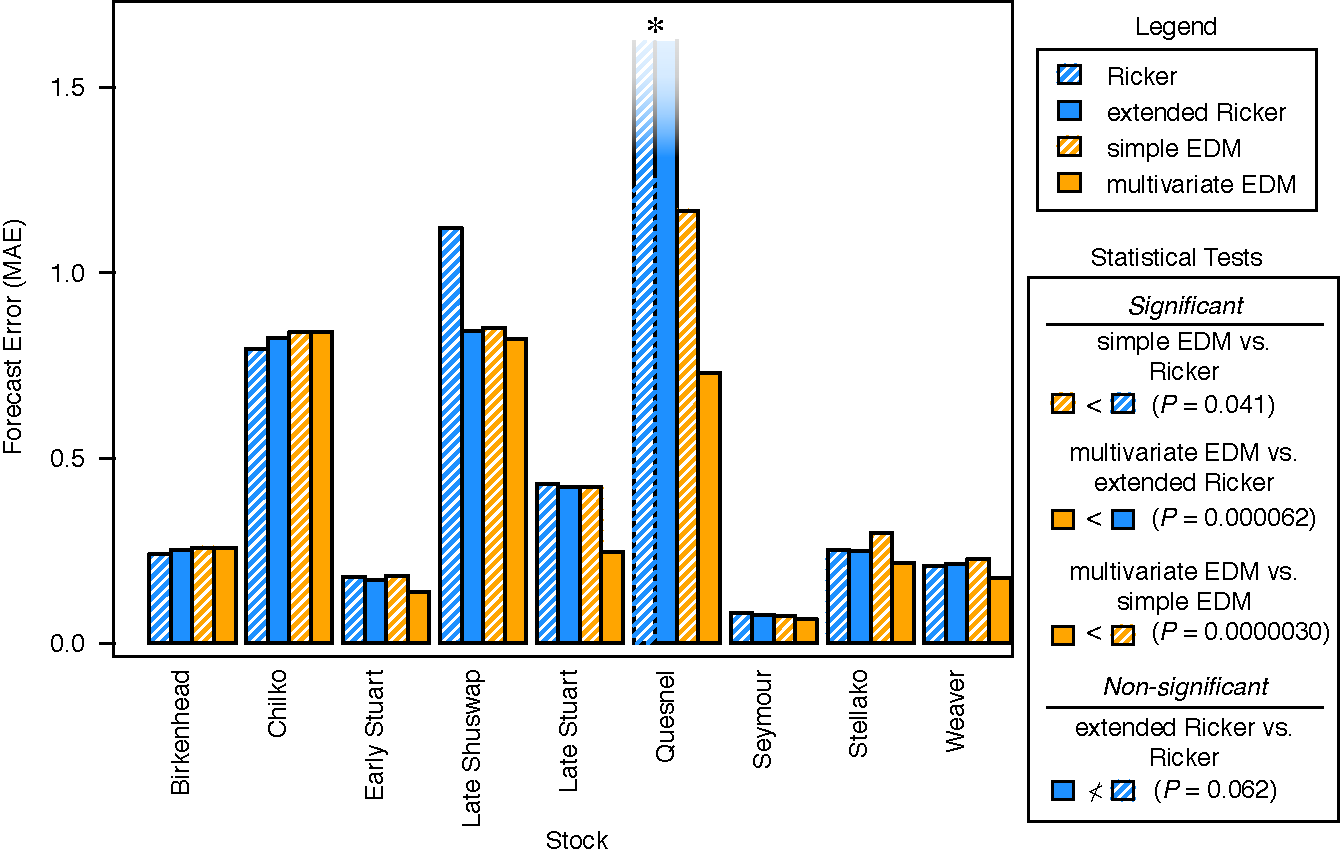
\includegraphics[width=\maxwidth{\textwidth}]{fig_salmon_s3.pdf}\end{center}
\caption[Comparison of forecast precision using MAE.]{\textbf{Comparison of forecast precision using MAE.}\newline
The simple EDM model has lower error than the equivalent Ricker model, [$t_{(493)} = -1.75$, $P = 0.041$]. Including environmental data significantly improves precision for the EDM models [$t_{(493)} = -4.58$, $P = 3.0\times10^{-6}$], but not for the Ricker models [$t_{(493)} = -1.54$, $P = 0.062$], and the resulting multivariate EDM models also have significantly lower error than the Ricker equivalents [$t_{(493)} = -3.87$, $P = 6.2\times10^{-5}$].\newline
\hspace{\linewidth}
* Note that the error for the Ricker and extended Ricker model extends beyond the upper range shown here. MAE is 2.13 for the Ricker model and 2.06 for the extended Ricker model.}
\label{fig_salmon_model_comparison_mae}
\end{figure}

\subsection{Possible Causal Mechanisms for SST, River Discharge, and the PDO}

The tested variables (river discharge, sea-surface temperature, the Pacific Decadal Oscillation) have been thought to influence sockeye salmon recruitment by being indicative of juvenile mortality in the early marine period (i.e., the first year of ocean residence) \cite{Beamish_2004}. For example, river discharge may improve multivariate EDM forecasts because of its effect on food availability, which is believed to play a role in determining this mortality \cite{Beamish_2012}. By affecting estuarine circulation in the Strait of Georgia, freshwater input (from the Fraser River and other riverine sources) can influence ocean productivity \cite{Beamish_1994}; indeed, river discharge, in combination with wind and other factors, has been linked to low oceanic productivity in the Strait of Georgia that may have contributed to poor returns of sockeye salmon in 2009 \cite{Beamish_2012, Thomson_2012}.

Using multivariate EDM, we do find support for river discharge as an informative variable, with the best EDM model for 4 of the 9 stocks containing river discharge as a coordinate (Table \ref{tab_salmon_forecast_skill}). Furthermore, for these 4 stocks (Early Stuart, Late Shuswap, Late Stuart, and Weaver), nearly all of the top-ranking EDM models include river discharge as a coordinate (i.e., Table \ref{tab_salmon_multivariate_full}). However, other than Late Stuart, there are EDM models excluding river discharge that have similar performance, suggesting that for Early Stuart, Late Shuswap, and Weaver, river discharge may be redundant if other observations of the environmental are available. Thus, while river discharge may be an informative variable, it does not appear to be strictly necessary for skillful predictions, except in the case of Late Stuart.

Pine Island SST also appears to be an important variable, and is included in the best multivariate model for 4 of the 9 stocks (Table \ref{tab_salmon_forecast_skill}). With Pine Island lighthouse located at the boundary between Queen Charlotte Strait and Queen Charlotte Sound (Figure \ref{fig_salmon_map}), the measured SST could be informative about the conditions that juvenile sockeye salmon experience after exiting the Strait of Georgia. That Pine Island SST can be informative about recruitment resonates with evidence that anomalous conditions in this area during 2007 were associated with low returns 2 years later (2009), while favorable conditions (low freshwater runoff and moderate northerly winds) in 2008 were associated with record high returns in 2010 \cite{Thomson_2012}. Here, only the Quesnel stock seems to require Pine Island SST for skillful forecasts, as the best model for Quesnel excluding this variable is much less skillful. For the remaining 3 stocks where the best EDM model included Pine Island SST, there were alternative multivariate EDM models including only other variables that showed very similar performance (Table \ref{tab_salmon_multivariate_full}). This suggests that the information in Pine Island SST relevant for predicting recruitment in these stocks may be duplicated in other environmental variables (see discussion in main text on non-uniqueness).

Lastly, although many studies \cite{Mantua_1997, Beamish_1997, Beamish_2004a} have found that decadal-scale climate and oceanic indicators, such as the PDO, are predictive of \emph{regional} productivity for Pacific salmon, one important question is whether this relationship holds at the individual stock level (i.e., do all stocks rise and fall in sync with one another). Among the Fraser River sockeye salmon, at least, there do not appear to be consistent patterns: there has been an overall decline since the early 1990s, but productivity for some stocks (e.g., Early Stuart) has been declining since the 1960s, while others (e.g., Late Shuswap, Weaver) have not exhibited a declining trend at all \cite{Grant_2010}. Our results similarly show no uniform effect of the PDO, as the best EDM model only includes the PDO as a coordinate for 2 of 9 stocks. In both cases (Stellako and Quesnel), however, performance is substantially improved when other variables are included compared to the model that includes just the PDO (Table \ref{tab_salmon_multivariate_full}). Thus, while the PDO may be informative for overall productivity of the Fraser River system, individual stocks appear to be sensitive to more localized environmental conditions; thus including additional (local) environmental variables is essential for improving forecasts for those stocks.

\begin{figure}[!ht]
\begin{center}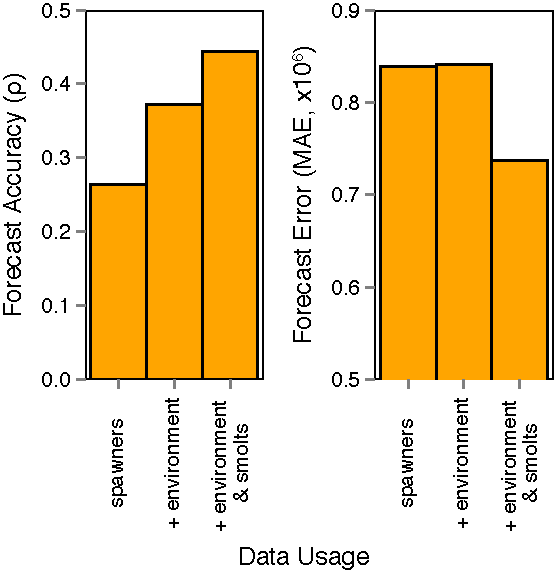
\includegraphics[width=\maxwidth{\textwidth}]{fig_salmon_s4.pdf}\end{center}
\caption[Including smolt data into the Chilko EDM model]{\textbf{Including smolt data into the Chilko EDM model}\newline
For the Chilko stock, adding smolt time series as a coordinate in the best environmental EDM model (spawners \& May Entrance Island SST \& the PDO) improves both accuracy and error.}
\label{fig_salmon_chilko_smolt_model}
\end{figure}

\subsection{Including Smolt Data into EDM Models}

For the Chilko stock, even an exhaustive search for the best possible multivariate EDM model did not produce very accurate forecasts ($\rho < 0.4$, Figure \ref{fig_salmon_chilko_smolt_model}). One possible explanation is that the relationship between spawner abundance and recruits is complex, such that a reconstruction using spawning stock and the tested environmental variables does not uniquely determine recruitment. In such cases, additional observations, such as other environmental factors or measures of salmon abundance at different ages, could resolve singularities in the reconstruction, thereby improving forecasts. For the Chilko stock, a long time series of smolt abundance is available, allowing us to include this variables as an additional coordinate in the multivariate EDM model (Equation \ref{eqn_chilko_smolt}, $J_t^\prime$ is smolt abundance normalized to the current cycle line). Testing this model, we found improvements in both accuracy and error (Figure \ref{fig_salmon_chilko_smolt_model}).

\begin{equation}
\label{eqn_chilko_smolt}
\vec{x}_t = \langle S_t^\prime, J_t^\prime, \mathrm{ET}_{t+2, \mathrm{May}}, \mathrm{PDO}_{t+2}\rangle
\end{equation}

Although the added expense of collecting this kind of data many not be reasonable for all stocks (particularly those that are already very predictable using the tested variables), these observations of sockeye at different ages are additional sources of information that could potentially improve forecasts, giving managers the ability to make trade-offs between data collection and predictability.

\subsection{Estimating Uncertainty for Simplex Projection Forecasts}

We note that the EDM models presented here produce point estimates for the number of returning sockeye salmon. However, fisheries management protocols often require an estimate of the uncertainty surrounding each forecast (i.e., confidence intervals) in order to evaluate the risks associated with management actions. Within the EDM framework, this uncertainty can be addressed in several ways. For example, the relative divergence of nearby trajectories in the reconstructed state space measures how sensitive the future will be to the current state, and is therefore directly indicative of forecast uncertainty. Here we demonstrate a simple implementation of this idea, by noting that the simplex projection method produces forecasts by computing a weighted average of the target variable, $y$ (equation \ref{eqn_simplex_scalar} from the main text):

\begin{equation*}
\hat{y}_{s+h} = \left(\sum_{i=1}^{b}{w_i\left(s\right)y_{n(s, i)+h}}\right) \bigg/ \sum_{i=1}^{b}{w_i\left(s\right)}. \tag{\ref{eqn_simplex_scalar} revisited}
\end{equation*}

In effect, the values of $y_{n(s, i)+h}$ can be thought of as the sample space for the desired prediction, where each value has probability $p_i(s) = \frac{w_i(s)}{\sum_{i=1}^{b}{w_i(s)}}$. Equation \ref{eqn_simplex_scalar} computes a forecast as the expected value of this probability mass function. This idea can then be extended to the second moment of this function in order to compute a variance:

\begin{equation}
\mathrm{Var}\left(\hat{y}_{s+h}\right) = \mathrm{E}\left[\left(y_{n(s, i)+h} - \hat{y}_{s+h}\right)^2\right] = \frac{\sum_{i=1}^{b}{w_i(s)\left(y_{n(s, i)+h} - \hat{y}_{s+h}\right)^2}}{\sum_{i=1}^{b}{w_i\left(s\right)}}
\end{equation}

Note that as the difference between each neighbor's forecast and the weighted average increases, variance will also increase, thus tracking the divergence of the nearest neighbors.

Because simplex projection is used to forecast relative age 4 and age 5 recruits, which are linearly combined to forecast returns (see Materials and Methods), we can similarly compute the variance of returns:

\begin{align}
\begin{split}
\mathrm{Var}\left(\hat{N}_t\right) &= \mathrm{Var}\left(\hat{R}_{4, t-4}\right) + \mathrm{Var}\left(\hat{R}_{5, t-5}\right) + \mathrm{Cov}\left(\hat{R}_{4, t-4}, \hat{R}_{5, t-5}\right)\\
\mathrm{Var}\left(\hat{R}_{a, t}\right) &= \mathrm{Var}\left(\hat{R}_{a, t}^\prime\right) \cdot \left(\sigma_k\left(R_a\right)\right)^2
\end{split}
\end{align}

Here, because the age 4 and age 5 recruits are computed from separate data, we can assume that the covariance is 0 (because the selection of nearest neighbors used to compute $\hat{R}_{4, t-4}$ are independent of those used to compute $\hat{R}_{5, t-5}$).

\begin{figure}[!ht]
\begin{center}\includegraphics[width=\maxwidth{\textwidth}]{fig_salmon_s5.pdf}\end{center}
\caption[Standard errors for EDM forecasts of Late Shuswap returns.]{\textbf{Standard errors for EDM forecasts of Late Shuswap returns.}\newline
Extending the simplex projection algorithm, standard errors for each forecast can be computed. Here, the predictions of the multivariate EDM model are plotted against observations for the Late Shuswap stock.}
\label{fig_salmon_standard_error}
\end{figure}

This is demonstrated in Figure \ref{fig_salmon_standard_error} for the best multivariate EDM model of the Late Shuswap stock. Plotting the EDM forecasts along with standard errors, it is clear that there is good correspondence: variability is higher for the dominant cycle line (as would be expected) and forecasts are generally within 1 standard error of the realized returns.

\section{Acknowledgments}
The authors thank Michael Fogarty, Terry Beacham, Brad Werner, Ethan Deyle, Charles Perretti, and two anonymous reviewers for their feedback on this work. This research is supported by a National Science Foundation Graduate Research Fellowship (HY), National Science Foundation Grant No. DEB-1020372 (GS, HY), Foundation for the Advancement of Outstanding Scholarship and Ministry of Science and Technology of Taiwan (CHH), NSF-NOAA Comparative Analysis of Marine Ecosystem Organization (CAMEO) program Grant NA08OAR\-4320894 / CAMEO (GS), the Sugihara Family Trust (GS), the Deutsche Bank-Jameson Complexity Studies Fund (GS), and the McQuown Chair in Natural Science (GS).

Chapter \ref{chap_salmon_environment}, in full, is a reprint of material published by the National Academies Press as: Hao Ye, Richard J. Beamish, Sarah M. Glaser, Sue C.H. Grant, Chih-hao Hsieh, Laura J. Richards, Jon T. Schnute, and George Sugihara. (2015) Equation-free mechanistic ecosystem forecasting using empirical dynamic modeling. \emph{Proceedings of the National Academy of Sciences} 112: E1569-E1576. The dissertation author was the primary investigator and author of this paper.
\chapter{Apparent Regime Shifts or Nonlinear State-Dependence?}
\label{chap_salmon_regimes}

\section{Abstract}
Natural systems that exhibit complex, nonlinear dynamics can undergo sudden changes characterized as regime shifts. A prominent example is the correlation between the Pacific Decadal Oscillation (PDO) and Pacific salmon, where salmon productivity is notably higher or lower depending on whether the PDO regime is warm or cold. Indeed, studies have found that salmon recruitment is better explained by separate stock-recruitment relationships for each PDO regime. However, this apparent relationship may actually represent a mirage correlation, a phenomenon known to occur when variables interact in a nonlinear system. Using nonparametric Empirical Dynamic Modeling (EDM), we fit  multivariate models to time series data of Fraser River sockeye salmon recruitment. We find no significant differences in forecasts when partitioning the data into different possible regimes, and thus no evidence supporting regime-specific recruitment dynamics. Rather, the observed correlation between the PDO and Pacific salmon productivity is likely a manifestation of nonlinear dynamics that gives the appearance of regime shifts even though the underlying system is unchanged.

\section{Introduction}

A central question in fisheries science, dating back at least a century to Hjort's seminal work \cite{Hjort_1914} is to understand the factors that influence recruitment. To date, various hypotheses have been proposed: tn the case of Pacific salmon populations, early work by Ricker on fitting stock-recruitment relationships suggested density-dependence as a mechanism \cite{Ricker_1954}. Another prominent hypothesis has been the influence of environmental variability on recruitment \cite{Cushing_1982}. Here, an early study by \cite{Ricker_1958}, again on Pacific salmon, found no evidence for environmental effects. However, this negative result may be caused by the limited statistical power of the data available at the time (Richard Beamish, personal communication, May 27, 2014).

More recent work has identified correlations between decadal scale climate indices (e.g., Pacific Decadal Oscillation, PDO; Aleutian Low Pressure Index, ALPI) and Pacific salmon productivity \cite{Mantua_1997, Beamish_1997}. These results suggest that there is indeed some form of physical-biological coupling between salmon populations and the environment. Indeed, when the data are partitioned by climate regime, standard stock-recruitment curves actually fit better for pink and sockeye salmon from the Fraser River \cite{Beamish_2004a}, suggesting that there are trends in survival and productivity related to climate.

One of the implications of regime-dependent behavior or parameters is that models will perform better when fit to data from exactly one regime (\`{a} la \cite{Beamish_2004a}). When the system transitions into a new regime, models based on data from a different regime may no longer be predictive. A correct understanding of the causes for observed shifts in populations is thus critical for fisheries management, to distinguish between natural impacts caused by biological or physical mechanisms, and fishing effects that could potentially be controlled through regulation and management \cite{Beamish_1999}. A failure to consider the possibility of changing system dynamics can lead to misguided or ineffective management, such as in the case of prolonged recovery of Northwest Atlantic cod \cite{Shelton_2011a}.

Although regime shifts appear quite common in marine fish stocks \cite{Vert-pre_2013}, the hallmark features of regime shifts are also characteristic of nonlinear systems. For example, time series from nonlinear systems often exhibit red noise power spectra, which can be erroneously identified as regime shifts \cite{Rudnick_2003}. Moreover, the defining feature of nonlinear systems is that variable interactions are state-dependent and change as a function of system state. Slow changes in the these interactions over time could be interpreted as regime shifts when linear models are applied, just as simple nonlinear functions can be approximated by piece-wise linear segments. Finally, a prime example of nonlinear phenomena that can give the appearance of changing dynamics is that of ``mirage correlations'', transient artifacts that can appear in coupled dynamic systems \cite{Sugihara_2012}. There is growing evidence that mirage correlations are prevalent in marine fisheries, with many studies showing inconsistent correlations as longer time series are collected \cite{Myers_1998, McClatchie_2010, Litzow_2014a}. Thus, the apparent regime-like behavior of Pacific salmon populations may not reflect changing behavior, but could actually be indicative of nonlinearity.

Here, we utilize the approach of empirical dynamic modeling (EDM) to examine the possibility of regime-dependent dynamics in Fraser River sockeye salmon. We consider four hypotheses for the number of distinct ``regimes'' over the time span of our data:
\begin{itemize}
\item[I] Four different time periods \cite{Beamish_2004a}: 1948-1976, 1977-1988, 1989-1998, and 1999-present
\item[II] Three different time periods \cite{Litzow_2014}: 1948-1976, 1977-1998, 1999-present
\item[III] Two different time periods \cite{McGowan_2003}: 1948-1976, 1977-present
\item[IV] One time period (null hypothesis): 1948-present
\end{itemize}

For each hypothesis, we fit multivariate EDM models \cite{Dixon_1999} to data from each time period separately, producing up to four different models. This procedure is then repeated for each of the nine most historically abundant stocks of sockeye salmon in the Fraser River: Birkenhead, Chilko, Early Stuart, Late Stuart, Late Shuswap, Quesnel, Seymour, Stellako, and Weaver. As shown in previous work \cite{Ye_2015}, EDM methods can accommodate nonlinearity as well as state-dependent environmental effects. Thus, this approach is ideally suited to distinguish between actual shifts in dynamics across hypothesized regimes and the illusion of change when linear models are applied to nonlinear systems.

\section{Results}

\begin{figure}[!ht]
\begin{center}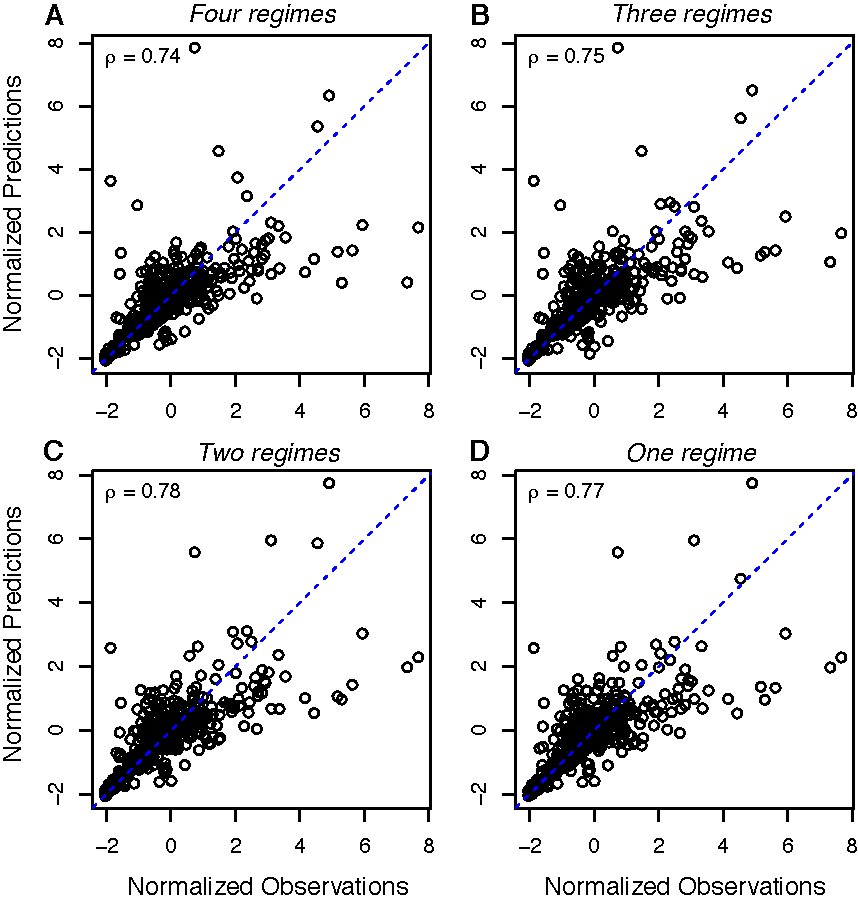
\includegraphics[width=\maxwidth{\textwidth}]{fig_regimes_1.pdf}\end{center}
\caption[Aggregated forecast accuracy for different regime hypotheses.]{\textbf{Aggregated forecast accuracy for different regime hypotheses.}\newline
(A) Normalized predictions vs. normalized observations, aggregated over the nine historically most abundant stocks. For each stock, models are fit separately to the four time periods of hypothesis I. (B-D) Same as (A), but for hypotheses II, III, and IV, respectively. Forecast skill is nearly identical across the four hypotheses, indicating no evidence for regime-specific behavior.}
\label{fig_regimes_aggregated_forecast_skill}
\end{figure}

Figure \ref{fig_regimes_aggregated_forecast_skill} shows predictions vs. observed values for the four different hypotheses and aggregated over the nine stocks examined here. Note that because the stocks have different mean population sizes, the forecasts and actual values for each stock are normalized to mean = 0, and variance = 1. It is visually apparent that there are very few differences in forecast skill across the four hypotheses, and confirmed by the computed forecast accuracy numbers ($\rho$, correlation coefficient between predicted and observed, in the upper left corner of each panel).

\begin{table}[!ht]
\caption[Stock-specific forecast skill for different regime hypotheses.]{\textbf{Stock-specific forecast skill for different regime hypotheses.}\newline
$\rho$, correlation coefficient between observations and predictions; MAE, mean absolute error.}
\label{tab_regimes_full_forecast_skill}
\begin{center}
\resizebox{\textwidth}{!}{
% latex table generated in R 3.2.0 by xtable 1.7-4 package
% Mon Aug 24 12:39:42 2015
\begin{tabular}{llrrrr}
  \hline
stock & metric & Four regimes & Three regimes & Two regimes & One regime \\ 
  \hline
Early Stuart & $\rho$ & 0.893 & 0.896 & 0.884 & 0.882 \\ 
  & MAE & 0.124 & 0.118 & 0.130 & 0.124 \\ 
  Seymour & $\rho$ & 0.781 & 0.777 & 0.775 & 0.762 \\ 
  & MAE & 0.056 & 0.057 & 0.056 & 0.058 \\ 
  Chilko & $\rho$ & 0.396 & 0.360 & 0.418 & 0.393 \\ 
  & MAE & 0.778 & 0.781 & 0.750 & 0.751 \\ 
  Late Stuart & $\rho$ & 0.760 & 0.750 & 0.794 & 0.791 \\ 
  & MAE & 0.316 & 0.316 & 0.296 & 0.304 \\ 
  Quesnel & $\rho$ & 0.554 & 0.603 & 0.706 & 0.705 \\ 
  & MAE & 1.068 & 1.029 & 0.916 & 0.925 \\ 
  Stellako & $\rho$ & 0.607 & 0.536 & 0.505 & 0.446 \\ 
  & MAE & 0.206 & 0.215 & 0.222 & 0.241 \\ 
  Birkenhead & $\rho$ & 0.572 & 0.615 & 0.538 & 0.481 \\ 
  & MAE & 0.180 & 0.171 & 0.189 & 0.213 \\ 
  Late Shuswap & $\rho$ & 0.873 & 0.886 & 0.872 & 0.867 \\ 
  & MAE & 0.840 & 0.809 & 0.887 & 0.880 \\ 
  Weaver & $\rho$ & 0.812 & 0.791 & 0.743 & 0.729 \\ 
  & MAE & 0.130 & 0.136 & 0.149 & 0.158 \\ 
   \hline
\end{tabular}

}
\end{center}
\end{table}

Table \ref{tab_regimes_full_forecast_skill} lists the forecast accuracy ($\rho$,  correlation coefficient between observations and predictions) and forecast error (MAE, mean absolute error) for each individual stock under the four different hypotheses. In general, there are no large differences in forecast skill across the four hypotheses. For some stocks (e.g., Quesnel, Birkenhead, Weaver), forecast skill is more variable across the different hypotheses; however, no pairwise comparisons are significant at the $p = 0.05$ level for either forecast accuracy ($\rho$) or forecast error (MAE) (see Methods for details of statistical tests).

\section{Discussion}

Our results (Figure \ref{fig_regimes_aggregated_forecast_skill} and Table \ref{tab_regimes_full_forecast_skill}) show no evidence that Fraser River sockeye salmon have regime-specific dynamics. This may not be surprising given that earlier studies in this system reported nonlinear dynamics and state-dependent environmental interactions \cite{Ye_2015}. However, even so, we might have expected forecasts to be better when different models could be fit separately to the different time periods. By selecting the best model for each time period, and using leave-one-out cross-validation to produce forecasts (see Methods), any differences in dynamics across regimes should appear as improvements in forecast skill. Given that performance was virtually identical across the four hypotheses, we conclude that there is no benefit to partitioning the data by climate regimes when modeling recruitment. Nevertheless, we consider several alternative explanations for our results.

\subsection{Alternative Explanations}

One possibility is that the nearest-neighbor forecasting method used in our EDM models is flexible enough to account for regime-specific dynamics, thus yielding equivalent performance for the``one-regime'' and ``multi-regime'' hypotheses. Because simplex projection makes predictions based on nearest neighbors (i.e., the historical times best judged to be similar states of the system) it could be the case that points from different regimes are simply accurately identified as \emph{not} being nearest neighbors. For example, the system behavior for the 1950-1976 time period could be quite different from that of the 1977-present time period, and when EDM is applied, the data from these two time periods are localized to different regions of the reconstructed state space. Thus, points in a different regime would not be selected as nearest neighbors, and forecast performance would be equivalent to fitting separate models to the different regimes. Even so, we might expect better forecasts when partitioning the data into regimes, because the model for each time period can be different. In other words, the most predictive set of environmental variables might be different across regimes, thereby yielding better forecast skill for the ``multi-regime'' hypothesis. However, this does not appear to occur, suggesting that there are no performance advantages to allowing the model to change over time.
%By selecting the best model for each time period, forecasts can improve in the ``multi-regime'' framework if the most predictive set of environmental variables changes.
%That this does not occur, suggests that in at least some cases, there are nearest neighbors selected from different time periods, thus providing an effective data advantage when fitting a single model to the entire time series.

Another possible explanation is that the variables used in this study are not informative enough to differentiate between regime-specific dynamics. As noted in \cite{Ye_2015}, these environmental variables are hypothesized to be proxies for juvenile food availability. Thus, while the relationship between recruitment dynamics and the tested environmental variables does not appear to be regime-specific, this may reflect the incompleteness of using an environmental measure as a proxy. In other words, it may be the case that the relationship between food availability and recruitment \emph{is} regime-specific, but that the mapping between food availability and the environmental proxies is not. As such, information is lost when using the environment as an imperfect proxy; this would explain both the imperfect forecast skill and the lack of improvement in forecasts when partitioning the data into different time periods. This data limitation could be overcome by including more direct measurements of the system. For instance trawl surveys of the Strait of Georgia should be more informative about actual food availability \cite{Beamish_2000}. Although these data do not extend far back enough to re-examine the regime shift question, it would still be possible to determine whether they are more relevant for predicting recruitment compared to indirect environmental proxies.

\subsection{Nonlinearity}

Like other studies \cite{Hsieh_2005, Glaser_2014}, our results contribute to growing evidence of nonlinear dynamics in marine fish stocks. An important distinction between the nonlinear perspective and that of the regime shift perspective relates to how data are used to construct models. In both frameworks, future behavior can be estimated by examining similar historical states. However, whereas the EDM approach identifies similar states based on location within the reconstructed state space, a regime shift perspective would identify similar states based on their proximity in time (i.e., points belonging to the same regime). In cases where the the system occupies similar regions of the state-space (perhaps due to red-noise spectra of important environmental factors), the resulting dynamics may thus appear to be time-dependent. In other words, the appearance of regime shifts can result from the nonlinear interaction of biological populations with red-noise-like environmental forcing.

We also note that aggregating data across multiple nonlinear systems is known to obscure nonlinear signals \cite{Sugihara_1994}. As such, the prominent correlations of Pacific salmon productivity with North Pacific climate \cite{Mantua_1997, Beamish_1997} may be a simplification of the true system behavior and the result of averaging over state-dependent interactions at the individual stock level. While such a coarse description of environmental impacts may be useful for predicting regional long-term trends (e.g., due to climate change), it ignores important nonlinear interactions that are potentially important for fisheries management on smaller spatial scales.

\section{Conclusions}

We find no evidence that Fraser River sockeye salmon dynamics change across different regimes of North Pacific Ocean climate. Rather, our results suggest that the apparent changes in mean salmon abundance reflect nonlinear interactions between stochastic environment and salmon biology. Moreover, because aggregating multiple nonlinear signals can result in linearity \cite{Sugihara_1994}, the observed correlations between salmon productivity and climate indices \cite{Mantua_1997, Beamish_1997} are likely the result of combining time series from multiple stocks into a single measure of \emph{regional} salmon productivity, and inadvertently diminishing the nonlinear signal.

The distinction between nonlinearity and regime-shift dynamics has important implications for fisheries management. If populations are influenced by the interaction of multiple factors (including fishing, the environment, and species interactions), correct accounting of these influences is necessary for effective management. As shown here, nonlinear, equation-free approach of EDM can accomplish the task of forecasting recruitment where traditional mathematical models would suggest that system behavior is tied to climate regimes. Nevertheless, the regime shift framework may be useful in some cases, for instance, when data are not available to identify nonlinear interactions. However, with sufficient observations, established patterns may eventually break down \cite{Litzow_2014a}, necessitating a more realistic and nonlinear worldview.

\section{Methods}

\subsection{Data}

Following \cite{Ye_2015}, we analyze yearly time series data for the 9 historically most abundant stocks (Birkenhead, Chilko, Early Stuart, Late Shuswap, Late Stuart, Quesnel, Seymour, Stellako, and Weaver) of sockeye salmon from the Fraser River system. Data span brood years 1948--2005, except for Late Stuart and Weaver, where data begin in 1949 and 1966, respectively.

Population data consists of two biological variables: stock size (number of effective female spawners) and recruitment (returning adults. Recruitment is also partitioned by age; following \cite{Grant_2010}, we consider only age 4 and age 5 recruits.

Environmental data consists of three variables: the Pacific Decadal Oscillation (PDO), sea-surface temperature (SST), and Fraser River discharge. As in \cite{Ye_2015}, one annual time series is constructed for the PDO as the average of monthly values from November to March \cite{Mantua_1997}, SST measures are monthly averages from two lighthouse stations (Entrance Island: April to June and Pine Island: April to July), and river discharge is measured at Hope (including both peak daily flow for the year, and monthly averages from April to June).

Because the identified regimes pertain to the physical conditions of the North Pacific, and the environmental data are believed to influence sockeye salmon recruitment at age 2, we partition the data according based on when the corresponding environmental measures fall in one regime or another. That is, if 1948-1976 is one physical regime, the relevant biological data for that regime corresponds to brood years 1946-1974, with age 4 recruits appearing in calendar years 1950-1978.

Data are partitioned in one, two, three, or four different time periods according to descriptions of North Pacific regimes in \cite{McGowan_2003, Beamish_2004a, Litzow_2014}:
\begin{itemize}
\item[I] Four different time periods: 1948-1976, 1977-1988, 1989-1998, and 1999-present
\item[II] Three different time periods: 1948-1976, 1977-1998, 1999-present
\item[III] Two different time periods: 1948-1976, 1977-present
\item[IV] One time period: 1948-present
\end{itemize}
As noted above, these years refer to calendar years for the physical environment. The corresponding brood years are shifted 2 years earlier.

\subsection{Model Construction and Performance}

Following \cite{Ye_2015}, we use multivariate simplex projection. For each combination of stock and time period, we examine models that include spawning stock size and up to 2 environmental variables. Forecasts for each model were produced using leave-one-out validation: for each forecast, the model was fit to data that excluded the corresponding stock size and environmental data. Although \cite{Ye_2015} used four-fold cross-validation to estimate out-of-sample forecast performance, several of the time periods examined here are much shorter and not suitable for such subdivision of the data.

Forecasts were produced for both age 4 and age 5 recruits before summing to obtain total recruitment for each brood year. (Note that this recruitment happens over two consecutive calendar years, with age 4 recruits appearing 4 years after spawning, and age 5 recruits appearing 5 years after spawning.) For each combination of stock and time period, the model producing the highest model accuracy ($\rho$, described below) was selected.

Model performance is quantified using Pearson's correlation coefficient ($\rho$) between observed and predicted returns as a measure of accuracy and MAE (mean absolute error) as a measure of error. Comparisons of $\rho$ between models uses a one-sided $t$ test with SE calculated using the HC4 estimator from \cite{Cribari-Neto_2004} and with adjusted degrees of freedom as suggested by \cite{Wilcox_2009}. Differences in MAE were computed using a paired $t$ test for the difference, treating each forecast as an independent sample.

To compute an aggregate statistic combining all 9 stocks, we first scale the observations and predictions for each stock so that the observed returns have mean $= 0$, variance $= 1$, and then combine the normalized values across stocks (Figure \ref{fig_regimes_aggregated_forecast_skill}).

\section{Acknowledgments}
This research is supported by Department of Defense, Strategic Environment Research and Development Program RC-2509 (GS, HY), Lenfest Ocean Program \#00028335 (GS), National Science Foundation Grant No. DEB-1020372 (GS, HY), NSF-NOAA Comparative Analysis of Marine Ecosystem Organization (CAMEO) program Grant NA08OAR4320894/CAMEO (GS), National Science Foundation Graduate Research Fellowships (HY), the Sugihara Family Trust (GS), the Deutsche Bank-Jameson Complexity Studies Fund (GS), and the McQuown Chair in Natural Science (GS).

Chapter \ref{chap_salmon_regimes}, in full, is material prepared for submission: Hao Ye and George Sugihara. Apparent regime shifts or nonlinear state-dependence: Environmental drivers of Fraser River sockeye salmon recruiment. The dissertation author was the primary investigator and author of this paper.
\chapter{Distinguishing Time-Delayed Causal Interactions Using Convergent Cross Mapping}
\label{chap_ccm_time_delays}

\section{Abstract}
An important problem across many scientific fields is the identification of causal effects from observational data alone. Recent methods (convergent cross mapping, CCM) have made substantial progress on this problem by applying the idea of nonlinear attractor reconstruction to time series data. Here, we expand upon the technique of CCM by explicitly considering time lags. Applying this extended method to representative examples (model simulations, a laboratory predator-prey experiment, temperature and greenhouse gas reconstructions from the Vostok ice core, and long-term ecological time series collected in the Southern California Bight), we demonstrate the ability to identify different time-delayed interactions, distinguish between synchrony induced by strong unidirectional-forcing and true bidirectional causality, and resolve transitive causal chains. 

\section{Introduction}

A fundamental question in science is identifying the causal relationships between variables. The conventional approach to this problem is to observe the outcomes of controlled experiments; however, this is not always possible due to moral, legal, or feasibility reasons. Consequently, the ability to infer causality using only observational data is a highly valuable tool with applications in many fields of study (e.g., financial systems, ecosystems, neuroscience \cite{Granger_1969, Hiemstra_1994, Chen_2006, Sugihara_2012}).

Early on, Bishop Berkeley \cite{Berkeley_1710} warned that the co-occurrence of events did not necessarily mean that they are causally related (i.e., correlation does not imply causation). Even so, the use of correlation to suggest causality (or more frequently, the lack of correlation suggesting no causality) has remained a common, heuristic notion, and is still commonly applied today. In 1969, however, Granger \cite{Granger_1969} suggested an alternative framework for detecting causality based on the idea of using prediction as a criterion. In the Granger causality framework, a variable $x$ is said to ``cause'' variable $y$ if $x$ has unique information (i.e., not found in other variables) that can improve the prediction of $y$. Thus, causality could be inferred if the optimal model for $y$ improves when $x$ is included. However, Granger noted that this approach might not apply in dynamic systems, and indeed, Sugihara et al. \cite{Sugihara_2012} showed that it does not: in dynamic systems with behaviors that are at least somewhat deterministic, information about past states is carried forward through time (i.e., the system is not completely stochastic). Thus, Takens' Theorem \cite{Takens_1981} applies, and so if $x$ is indeed causal to $y$, then information about $x$ must be recorded in $y$. Consequently, causal variables (i.e., $x$) cannot contain unique information (it will also be recorded in the affected variables), and so Granger's test is invalid (except in certain cases; see Discussion). 

As an alternative test for causality, Sugihara et al. \cite{Sugihara_2012} suggested a new method, convergent cross mapping (CCM). It follows from Takens' Theorem \cite{Takens_1981} that if $x$ does influence $y$, then the historical values of $x$ can be recovered from variable $y$ alone. In practical terms, this is accomplished using the technique of ``cross mapping'': a time delay embedding is constructed from the time series of $y$, and the ability to estimate the values of $x$ from this embedding quantifies how much information about $x$ has been encoded into $y$. Thus, the causal effect of $x$ on $y$ is determined by how well $y$ cross maps $x$. This approach is described in further detail in the materials and methods, but also summarized in this short instructional animation: (\url{https://www.youtube.com/playlist?list=PL-SSmlAMhY3bnogGTe2tf7hpWpl508pZZ}).

Although CCM can be successfully applied to systems with weak to moderate coupling strengths, Sugihara et al. observed that exceptionally strong unidirectional forcing can lead to the phenomenon of ``generalized synchrony'' \cite{Rulkov_1995}. In these situations, the dynamics of a response variable, $y$, become dominated by those of the driving variable, $x$, such that the full system (consisting of both the response variable and driving variable) collapses to just that of the driving variable. Although there is no causal effect of $y$ on $x$, the states of the driving variable $x$ can uniquely determine the response variable $y$, and so CCM is observed in both directions (i.e., $x$ cross maps $y$ and $y$ cross maps $x$). Thus, CCM appears to be limited by the fact that it may not be able to distinguish between bidirectional causality and strong unidirectional causality that leads to synchrony.

Here, we propose an extension to CCM that can resolve this problem: by explicitly considering different lags for cross mapping, it is possible to determine whether a driving variable acts with some time delay on a response variable. In the case of synchrony caused by strong unidirectional forcing, this approach should detect a negative lag for cross mapping in the true causal direction (the response variable is better at predicting the past values of the driving variable rather than future values) and a positive lag in the other direction (the driving variable best predicts the future response). Thus, this ``asynchrony'' reflecting the time lag in the response can be used to distinguish between bidirectional causality and generalized synchrony when there is a detectable lag in the response time between causes and effects.

This extension of CCM has several additional applications: the identification of time delays in causation can be informative, for instance in understanding delays in interventions or manipulations. It can also be used to identify the causal effects of stochastic drivers that have no dynamics (for which general cross mapping may not succeed), and can even correctly determine the order of variables in a transitive causal chain.

\section{Results \& Discussion}

\subsection{Model Simulations}

\begin{figure}[!ht]
\begin{center}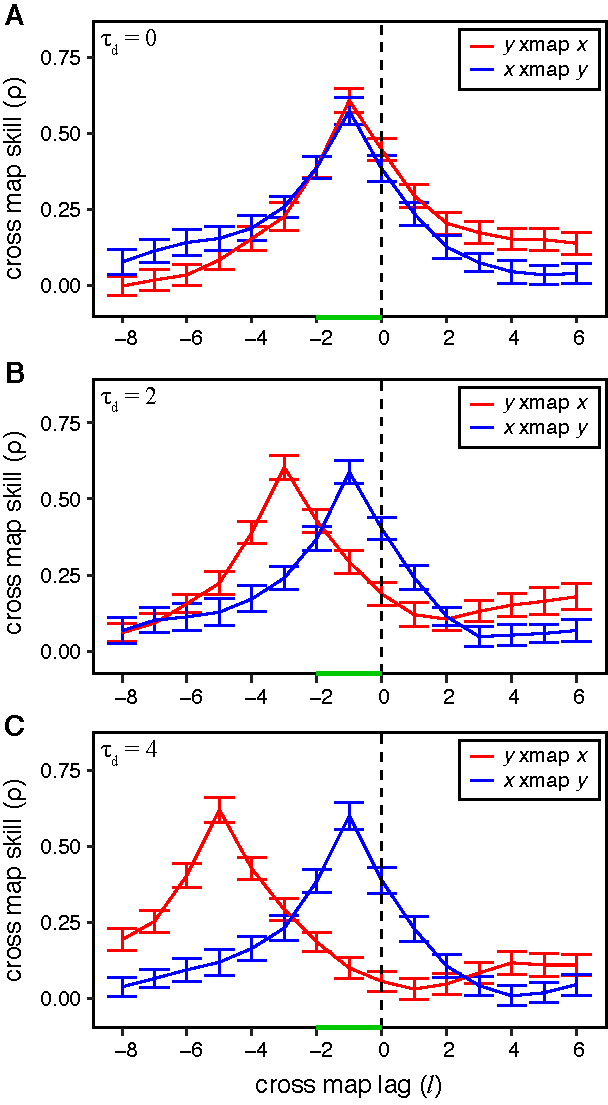
\includegraphics[scale = 0.7]{fig_lag_2sp_delay.pdf}\end{center}
\caption[Model demonstration of causal lags and optimal cross mapping using a 2-species logistic model with bidirectional forcing.]{\textbf{Model demonstration of causal lags and optimal cross mapping using a 2-species logistic model with bidirectional forcing.}\newline
Cross-mapping skill ($\rho$) is shown as a function of cross-mapping lag for three different time delays, $\tau_d$, in the effect of $x$ on $y$. Here, ``$y$ xmap $x$'' refers to using $y$ and its lags to cross map variable $x$ with time lag $l$. (A) With $\tau_d = 0$, both variables respond to each other within a single time-step ($y(t+1)$ is influenced by $x(t)$ and vice-versa), and so the optimal cross map lag occurs at $l = -1$, falling within the embedding vector (green bar) as expected. (B-C) For $\tau_d = 2$ or 4, the effect of $x$ on $y$ is delayed, and so the optimal lag for $y$ cross mapping $x$ (i.e., red line, measuring the effect of $x$ on $y$) shifts back by a corresponding amount, while $x$ cross mapping $y$ is unchanged. Plots show mean cross map skill and standard deviation over 100 random libraries (see Materials and Methods).}
\label{fig_lag_2sp_delay}
\end{figure}

Figure \ref{fig_lag_2sp_delay} shows the results of extended CCM applied to the two-species coupled logistic map (equation \ref{eqn_2sp_delay}). As shown in the first panel (Figure \ref{fig_lag_2sp_delay}A), where causation occurs with an effective delay of 1 time step ($y(t)$ affects $x(t+1)$ and vice-versa), the optimal cross mapping in both directions occurs at a lag of -1. Moreover, as expected, a time delay in the effect of $x$ on $y$ (Figure \ref{fig_lag_2sp_delay}B-C), produces optimal cross mapping (from $y$ to $x$) with a lag corresponding to the degree of time delay. Extending this analysis to systems with random coefficients (see Supplementary Information), the result is robust, with only a few outliers that exhibit optimal cross mapping at different lags (Figure \ref{fig_lag_2sp_delay_rand}). This validates a basic rule of thumb for bidirectional causality: we may reasonably expect optimal cross mapping lags to be negative, and with the magnitude of the lag roughly equal to the time delay of causality.

\begin{figure}[!ht]
\begin{center}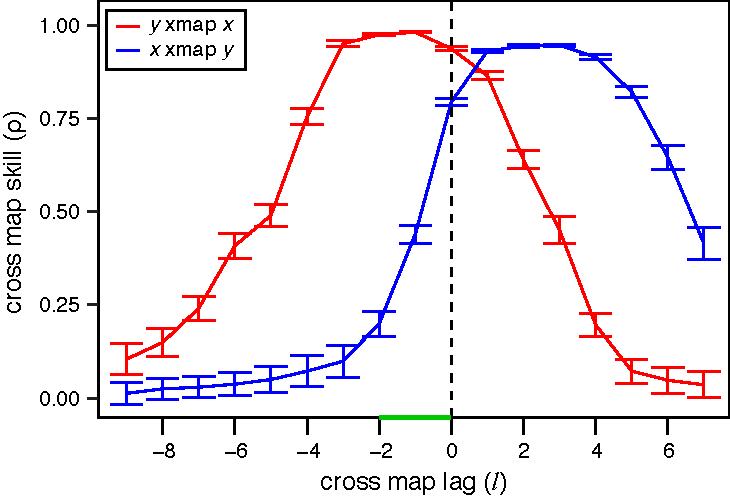
\includegraphics[width=\maxwidth{\textwidth}]{fig_lag_2sp_synch.pdf}\end{center}
\caption[Generalized synchrony in a 2-species logistic model with unidirectional forcing.]{\textbf{Generalized synchrony in a 2-species logistic model with unidirectional forcing.}\newline
In this system, the dynamics of $y$ becomes enslaved to $x$, and so $y$ can be predicted from $x$. Since $x$ affects future values of $y$, $x$ is best able to cross map $y$ forward in time ($l \sim 3 > 0$), whereas cross mapping in the true direction shows optimal prediction for negative time lags ($l \sim -1 < 0$, as in Figure \ref{fig_lag_2sp_delay}). Thus, even though there is cross mapping in both directions, we can use the positive optimal prediction lag to distinguish the direction of causality. As in Figure \ref{fig_lag_2sp_delay}, ``$y$ xmap $x$'' refers to using $y$ and its lags to cross map variable $x$ with time lag $l$; plots show mean cross map skill and standard deviation over 100 random libraries (see Materials and Methods).}
\label{fig_lag_2sp_synch}
\end{figure}

For systems where strong unidirectional causality leads to generalized synchrony (equation \ref{eqn_2sp_synch}), a time delay in the response can be detected using extended convergent cross mapping. Although the response variable ``synchronizes'' to the causal variable, if causality is not instantaneous, the synchronization occurs with some lag that can then be identified using extended convergent cross mapping. In Figure \ref{fig_lag_2sp_synch}, we find that the optimal cross map lag from $y$ to $x$ is negative, as expected; $x$ causes $y$, and so cross map skill is better when estimating the historical influence of $x$ from the response variable $y$. Conversely, the optimal cross map lag from $x$ to $y$ is positive, because even with synchrony, there is no flow of causal information from $y$ to $x$, and so changes in $x$ are not reflected in $y$ until sometime in the future. Thus, the positive lag from $x$ cross mapping $y$ informs us that there is unidirectional causality, even when the interaction is strong enough to result in synchrony. Again, extending this analysis to similar systems with random coefficients (see Supplementary Information), we find that optimal cross map lags can reliably distinguish between generalized synchrony and bidirectional causality (Figure \ref{fig_lag_2sp_synch_rand}).

\begin{figure}[!ht]
\begin{center}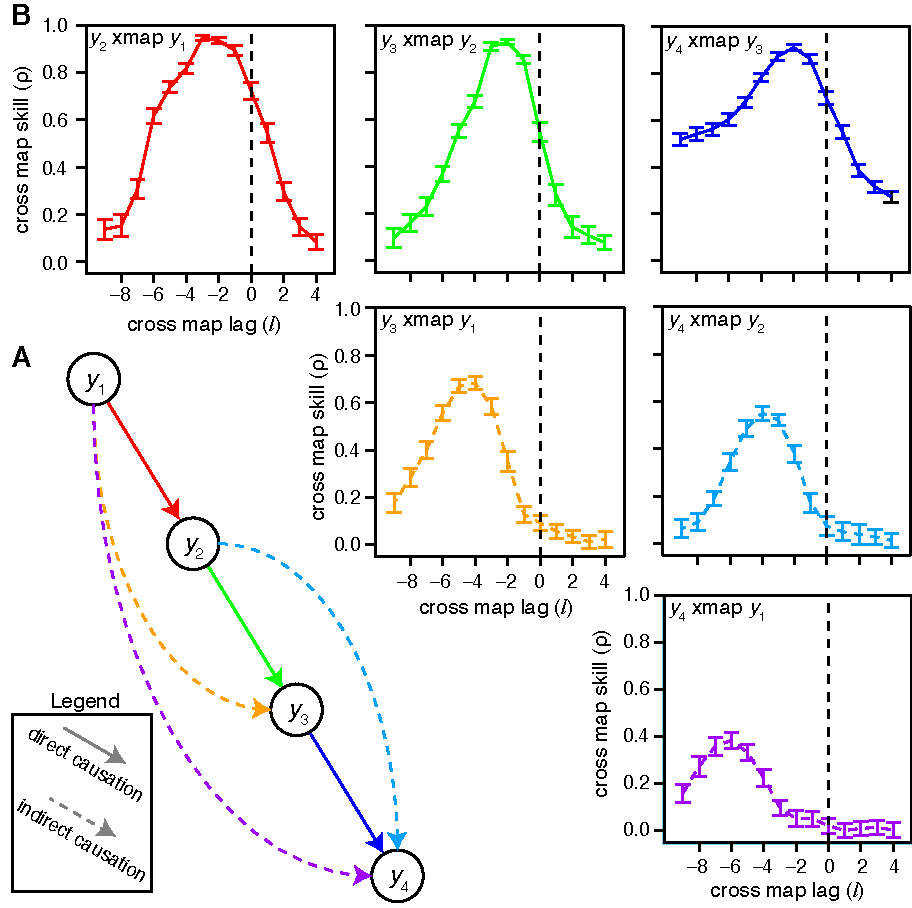
\includegraphics[width=\maxwidth{\textwidth}]{fig_lag_4sp_transitive.pdf}\end{center}
\caption[Direct and indirect causality in a transitive causal chain.]{\textbf{Direct and indirect causality in a transitive causal chain.}\newline
(A) In this system, $y_1$ causes $y_2$ causes $y_3$ causes $y_4$ such that indirect causation from $y_1$ to $y_3$, $y_2$ to $y_4$, and $y_1$ to $y_4$ occurs. (B) Using extended CCM, the direct links (top row) are strongest with the highest cross map skill and the most immediate effects ($l \sim -2$), the indirect links separated by one node (middle row) have moderate cross map skill and somewhat delayed effects ($l \sim -4$), and the indirect link from $y_1$ to $y_4$ (bottom row) is the weakest and with the longest time delay ($l \sim -6$). Here ``$y_i$ xmap $y_j$'' refers to using $y_i$ and its lags to cross map to $y_j$. Plots show mean cross map skill and standard deviation over 100 random libraries (see Materials and Methods).}
\label{fig_lag_4sp_transitive}
\end{figure}

As discussed by Sugihara et al. \cite{Sugihara_2012}, CCM can detect indirect causality that occurs through a transitive causal chain. For example, in the system depicted in Figure \ref{fig_lag_4sp_transitive}A, $y_1$ causes $y_2$ causes $y_3$ causes $y_4$ (equation \ref{eqn_4sp_transitive}). With CCM, we can detect these direct causal connections (e.g., using the cross map from $y_j$ to $y_i$ to infer the effect of $y_i$ on $y_j$). However, there are also indirect effects from $y_1$ to $y_3$, $y_2$ to $y_4$, and $y_1$ to $y_4$. These indirect effects may also appear significant in CCM if coupling is strong enough. To unravel the direct from indirect effects in this system, we can apply extended CCM to identify the optimal cross map lags and optimal cross map skill (Figure \ref{fig_lag_4sp_transitive}B). For the direct links (top row of Figure \ref{fig_lag_4sp_transitive}B), optimal cross mapping occurs with high skill and a small negative lag ($l \sim -2$); for indirect links separated by a single node (middle row of Figure \ref{fig_lag_4sp_transitive}B), optimal cross mapping occurs with moderate skill and a moderate negative lag ($l \sim -4$); and for the indirect link from $y_1$ to $y_4$ (separated by both $y_2$ and $y_3$), optimal cross mapping is weak, and at a large negative lag ($l \sim -6$). When this analysis was repeated for model systems with random coefficients (see Supplementary Information), the differences in optimal cross map lag were relatively robust (Figure \ref{fig_lag_4sp_transitive_rand}). However, cross map skill showed more variance, suggesting that it is a less reliable indicator of direct vs. indirect causation. The outliers are likely a result of stable dynamics (with cross map skill, $\rho$ that reaches 1), since this is a simple model simulated without process error.

\begin{figure}[!ht]
\begin{center}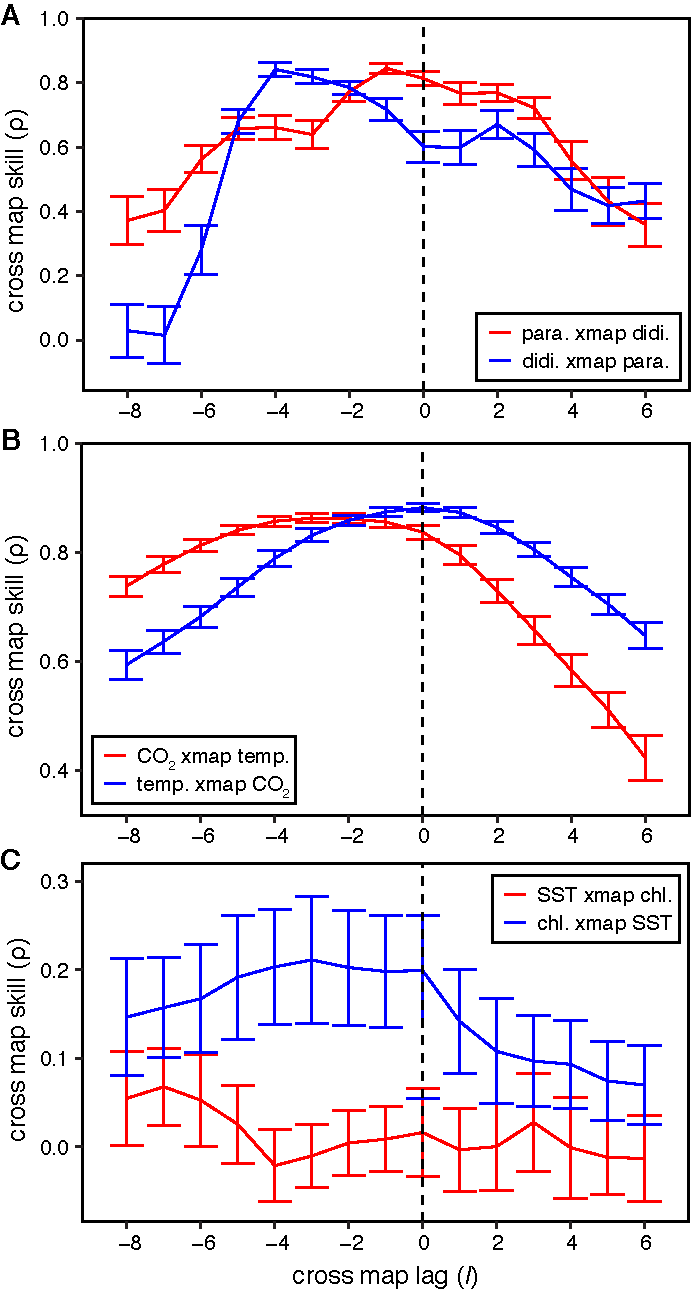
\includegraphics[scale = 0.55]{fig_lag_real_examples.pdf}\end{center}
\label{fig_lag_real_examples}
\caption[Applying extended CCM to real world examples.]{\textbf{Applying extended CCM to real world examples.}\newline
(A) Extended CCM analysis of time series from Veilleux's predator-prey experiment \cite{Veilleux_1976} with \emph{Paramecium aurelia} (prey) and \emph{Didinium nasutum} (predator) reveals bidirectional causality. While the effect of predators on prey (red, ``para. xmap didi.'') is immediate, the effect of prey on predators (blue, ``didi. xmap para.'') shows a distinct lag, as prey ingestion does not instantaneously translate into population growth. (B) Analysis of causality between Earth atmospheric CO$_2$ and temperature using time series data from the Vostok ice core for the previous 412,000 years. As expected CO$_2$ has a nearly instantaneous effect on temperature (blue, ``temp. xmap CO$_2$'') due to the fast-acting greenhouse gas effect, while the influence of temperature on CO$_2$ is much slower, with an optimal CCM lag of $\sim 3000$ years (red, ``CO$_2$ xmap temp.''). (C) Analysis of weekly averages of sea surface temperature (SST) and chlorophyll-a at SIO pier in La Jolla, CA suggests that the effect of SST occurs with a lag of 1-4 weeks (blue, ``chl. xmap SST''). All plots show mean cross map skill and standard deviation over 100 random libraries (see Materials and Methods).}
\end{figure}

\subsection{Veilleux's Paramecium-Didinium Experiment}

Applying extended CCM to the time series of \emph{Paramecium} and \emph{Didinium} from Veilleux's lab experiments \cite{Veilleux_1976}, we confirm the results of Sugihara et al. \cite{Sugihara_2012} showing bidirectional causality. However, whereas Sugihara et al. suggested that the difference in cross mapping predictability (with a lag of 0) was indicative of stronger top-down forcing, our analysis here reveals another layer to the story: considering different lags, we find that cross mapping predictability is roughly equal at optimal lag values (Figure \ref{fig_lag_real_examples}A), suggesting that top-down and bottom-up effects are equally important. We do note that the optimal cross mapping lag does depend on the interaction: an optimal lag of -1 for the \emph{Paramecium} cross mapping \emph{Didinium} direction suggests that \emph{Paramecium} respond quickly to changes in \emph{Didinium} abundance. However, an optimal lag of -4 for the \emph{Didinium} cross mapping \emph{Paramecium} direction suggests that \emph{Didinium} respond more slowly to changes in \emph{Paramecium} abundance. These results are consistent with the ecological context of this system \cite{Li_2013}: the prey (\emph{Paramecium}) respond quickly to predators (\emph{Didinium}) because predator-induced mortality has an immediate (negative) effect on the abundance of prey, whereas the abundance of predators (\emph{Didinium}) responds more slowly to prey (\emph{Paramecium}), because of the time delay in converting food into new individuals.

\subsection{Vostok Ice Core}

Figure \ref{fig_lag_real_examples}B shows the application of extended convergent cross mapping to time series of CO$_2$ and temperature reconstructed from the Vostok ice core \cite{Petit_1999}. Here, we detect bidirectional causality (the optimal cross mapping lag is negative in both directions), suggesting that there is a positive feedback in the Earth's climate system between temperature and greenhouse gases. Notably, the optimal lag in the temperature to CO$_2$ direction matches current scientific knowledge that greenhouse gases have a rapid effect on temperature (faster than the 1000-year timescale of the data), while the influence of global temperature on greenhouse gases likely occurs through slower mechanisms (e.g., increased plant respiration at higher temperatures \cite{Cramer_2001}, release of greenhouse gases from terrestrial \cite{Schuur_2009} or marine ecosystems \cite{Archer_2009}). A detailed analysis of this system appears in van Nes et al. \cite{Nes_2015}.

\subsection{Southern California Bight}

In Figure \ref{fig_lag_real_examples}C, we show the results of extended CCM applied to long-term time series of chlorophyll-a and sea surface temperature measured at the Scripps Institution of Oceanography pier. As expected, there is no effect of chlorophyll-a on SST (red line). However, we do identify a causal influence of SST on chlorophyll-a, suggesting that the physical environment plays a role in determining phytoplankton abundances (which are proxied by concentrations of chlorophyll-a). Moreover, optimal cross mapping occurs with a lag of 3 weeks, suggesting that the physical drivers of algae populations act with a lag of several weeks. Ideally, if other causal drivers show similar time delays in their effects, then it may be possible to produce models that can forecast events such as algal blooms several weeks in advance!

\subsection{Stochastic Drivers}

We note that in certain systems, especially those with stochastic drivers that contain unique information, Granger causality may correctly identify causal interactions. Indeed, Granger causality has been successful when applied to system consisting solely of stochastic components. However, in situations where both cause and effect have deterministic dynamics, causal information cannot be isolated from amongst the affected variables, and alternative methods, such as CCM must therefore be used.

\subsection{Final Remarks}

Here, we have shown that explicitly considering time lags when applying convergent cross mapping can be a valuable tool beyond the simple test of whether two variables are causally related. Although this general approach has been explored elsewhere \cite{Schumacher_2015}, here we show how the CCM framework can be directly extended to account for temporal delays. As demonstrated in our model simulations, CCM can now distinguish synchrony induced by strong unidirectional forcing from true bidirectional causation (Figure \ref{fig_lag_2sp_synch}), as well as order nodes in transitive causal chains that produce direct and indirect causal links (Figure \ref{fig_lag_4sp_transitive}). 

In addition, we show how identification of time delays can clarify our understanding of the causal effects, which can be valuable in producing a more detailed and mechanistic description of causal dynamics in real systems. For example, knowing the approximate time delay of causal interactions can be important when forecasting future events -- although in general, a single time series contains all necessary dynamic information, this will not be the case when stochastic drivers are influencing the dynamics. Since the stochastic driver has unique information, it must be explicitly included at the appropriate lag for optimal predictability (see ref. \cite{Deyle_2013, Ye_2015} for examples). Moreover, understanding the delayed effect of external drivers will be important in management scenarios, as knowing when to expect the system to respond to interventions or manipulations will guide future management actions.

\section{Methods}

\subsection{Convergent Cross Mapping}

The basic principle of cross mapping involves reconstructing system states from two time series variables and then quantifying the correspondence between them using nearest neighbor forecasting \cite{Sugihara_1990}. Reconstruction is done using the method of time delay embedding: with the system state represented using successive lags of a single time series \cite{Takens_1981, Packard_1980}. For example, given a time series $\{y(t)\}$, an $E$-dimensional reconstruction uses $E$ successive lags of $y$, each separated by a time step $\tau$: $\langle y(t), y(t-\tau), \dots, y(t - (E-1)\tau) \rangle$.

We note that the optimal value of the embedding dimension $E$ depends on several factors, including system complexity, time series length, and noise. In the case of model systems, the number of interacting variables is known exactly and was used to select $E$. In the remaining cases, the value of $E$ was determined empirically by applying simplex projection \cite{Sugihara_1990} to the individual time series and choosing the optimal $E$. Since most time series were not overly sampled in time, we fixed $\tau = 1$ for all systems. 

In the case of a system where $x$ causes $y$, Takens' Theorem \cite{Takens_1981} implies that there should be a correspondence between the state $\vec{y}(t)$ and the contemporaneous state $\vec{x}(t)$. Convergent cross mapping (CCM \cite{Sugihara_2012}) quantifies this relationship using simplex projection (a nearest-neighbor forecasting method, see ref. \cite{Sugihara_1990} for details) to estimate the scalar value $x(t)$ from the reconstructed vector $\vec{y}(t)$ (see ref. \cite{Sugihara_2012} and Movie S3 for details). Although different performance metrics are possible, here we use Pearson's correlation coefficient between the estimated and observed values of $x(t)$ as an indicator of ``cross map skill''.

We note that, in general, one may compute a function that maps from $\vec{y}(s)$ to the entire vector $\vec{x}(s)$ as opposed to just the scalar value $x(s)$ \cite{Schiff_1996, Ma_2014}. However, doing so can decrease the sensitivity of the cross mapping idea, because the errors are no longer scalar values, but $E$-dimensional vectors, for which common distance metrics can become meaningless \cite{Aggarwal_2001}. Moreover, by estimating entire vectors, we limit the capability to use cross mapping to analyze time delays in the effect of $x$ on $y$, which we show here can be informative in an extended version of CCM (see below).

\subsection{Extended Convergent Cross Mapping}

\begin{figure}[!ht]
\begin{center}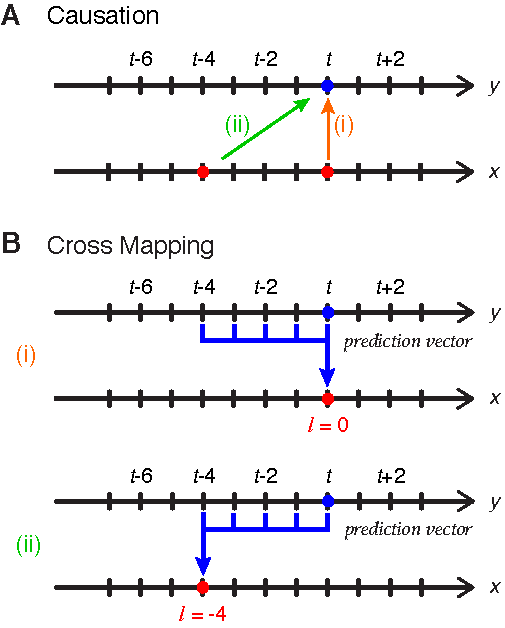
\includegraphics[width=\maxwidth{\textwidth}]{fig_lag_extended_ccm.pdf}\end{center}
\caption[Effect of time delays on cross mapping.]{\textbf{Effect of time delays on cross mapping.}\newline
Panel A shows causation for two cases: (i) no time delay in the effect of $x$ on $y$ (i.e., $y$ responds instantaneously to $x$), and (ii) $y$ responds to $x$ with a time delay of 4 (time steps). Panel B shows (i) cross mapping with $l = 0$, equivalent to the original formulation by Sugihara et al. \cite{Sugihara_2012} and (ii) cross mapping with $l = -4$, which may be expected to be better than $l = 0$ when $x$ acts on $y$ with some time delay.}
\label{fig_lag_real_examples}
\end{figure}

Standard cross mapping when $x$ causes $y$ (Figure \ref{fig_lag_real_examples}A) computes the predictability of $x(t)$ from the $E$-dimensional reconstruction $\vec{y}(t) = \langle y(t), y(t-\tau), \dots, y(t - (E-1)\tau) \rangle$ (Figure \ref{fig_lag_real_examples}B.i). However, the general theory of CCM \cite{Sugihara_2012}, based on generalizations of Takens' Theorem \cite{Sauer_1991, Deyle_2011}, suggests that we should also be able to cross map from $\vec{y}(t)$ to $x(t+l)$, for any reasonable lag value of $l$, since the variable $x(t+l)$ is simply another observation function of the system. In fact, if $x$ acts on $y$ with some time delay (Figure \ref{fig_lag_real_examples}A.ii), then the current state of the system, $\vec{y}(t)$, will better predict the past values of $x$ (Figure \ref{fig_lag_real_examples}B.ii).

In general, we note that optimal predictability may be expected to occur for some $l < 0$, even if $y$ responds instantaneously to $x$ \cite{Casdagli_1991}. In other words, the state of the system at a time $t$ is often best estimated from a reconstruction that includes both past and future values. This phenomenon occurs because information in a dynamic system can be thought of as propagating both forwards and backwards through time. In other words, knowing the exact value of variable $x$ at time $t$ restricts the likely set of possible futures (the value at time $t+1$) as well as the likely set of possible pasts (the state at time $t-1$). Furthermore, the exact amount of information contained in past (and future) values of $x$ is determined by the rate at which predictability decreases when we forecast further into the future (or past). Consequently, this means the most information about the current system state occurs with a combination of forward and backward lags \cite{Casdagli_1991}: a time-centered embedding that balances positive and negative lags: $\langle y(t), y(t-\tau), y(t+\tau), \dots y(t-(E-1)\tau/2), y(t+(E-1)\tau/2) \rangle$. In the context of extended CCM, this then suggests that the optimal lag will occur in the middle of the prediction vector: $l = (E-1)\tau/2$. In reality, however, the optimal lag will vary from system to system; so while the ``middle of the vector'' is a useful heuristic, optimal cross mapping at any lag that lies within the embedding vector, $-(E-1)\tau \le l \le 0$, is consistent with an influence of $x$ on $y$ with no time delay.

\subsection{Two-Species Model System with Bidirectional Causality}

We first consider a simple model system consisting of 2 coupled logistic difference equations:
\begin{align}
\label{eqn_2sp_delay}
\begin{split}
x(t+1) &= x(t) \left[3.78 - 3.78 x(t) - 0.07 y(t)\right]\\
y(t+1) &= y(t) \left[3.77 - 3.77 y(t) - 0.08 x(t-\tau_d)\right]
\end{split}
\end{align}
where $\tau_d$ is the time delay for the effect of $x$ on $y$. The system is initialized as $x(1) = 0.2$ and $y(1) = 0.4$, and run for 3000 time steps, with different values for the time delay: $\tau_d = 0$, $\tau_d = 2$, and $\tau_d = 4$. Using extended CCM, we analyze this system using $E = 2$, $\tau = 1$, selecting 100 random libraries of 200 vectors over time points 101-2000, and computing cross map skill for time points 2001-3000.

\subsection{Two-Species Model System with Synchrony}

We also examine a modified form of the above system with causality from $x$ to $y$ only:
\begin{align}
\label{eqn_2sp_synch}
\begin{split}
x(t+1) &= x(t) \left[3.8 - 3.8 x(t)\right]\\
y(t+1) &= y(t) \left[3.1 - 3.1 y(t) - 0.8 x(t)\right]
\end{split}
\end{align}
As above, the system is initialized as $x(1) = 0.2$ and $y(1) = 0.4$, and run for 1000 time steps. Because of the strong forcing of $x$ on $y$, the dynamics of $y$ are entrained to those of $x$ (i.e., ``generalized synchrony'' \cite{Rulkov_1995}). Thus, we apply extended CCM to identify the optimal cross map lag and distinguish this case from the case of bidirectional causality. In this system, we also use $E = 2$, $\tau = 1$, selecting random libraries of 200 vectors over time points 101-2000, and computing cross map skill for time points 2001-3000.

\subsection{Four-Species Model System}

To demonstrate extended CCM in systems with indirect causality (as a result of a transitive causal chain), we consider a 4-species model system. The system is initialized as $y_1(1) = y_2(1) = y_3(1) = y_4(1) = 0.4$, and evolves according to:
\begin{align}
\label{eqn_4sp_transitive}
\begin{split}
y_1(t+1) &= y_1(t) \left[3.9 - 3.9 y_1(t)\right]\\
y_2(t+1) &= y_2(t) \left[3.6 - 0.4 y_1(t) - 3.6 y_2(t)\right]\\
y_3(t+1) &= y_3(t) \left[3.6 - 0.4 y_2(t) - 3.6 y_3(t)\right]\\
y_4(t+1) &= y_4(t) \left[3.8 - 0.35 y_3(t) - 3.8 y_4(t)\right]
\end{split}
\end{align}

Although the only direct causal links are from $y_1$ to $y_2$, from $y_2$ to $y_3$, and from $y_3$ to $y_4$, this creates a transitive chain of causality, such that there is an indirect influence of $y_1$ on $y_3$, from $y_2$ to $y_4$, and from $y_1$ to $y_4$ (Figure \ref{fig_lag_4sp_transitive}a). Thus, we apply extended CCM with $E = 4$ and $\tau = 1$ to distinguish between direct and indirect causation. For each pair, we sample 100 random libraries of size 200 from time points 101-1000 and compute the cross map skill for time points 2001-3000.

\subsection{\emph{Paramecium}-\emph{Didinium} Predator-Prey System}

We examine causality in a classical predator-prey system, the \emph{Paramecium}-\emph{Didinium} protozoan system using experimental time series from Veilleux \cite{Veilleux_1976}, who refined earlier work from Gause \cite{Gause_1935} and Luckinbill \cite{Luckinbill_1973} to establish sustained oscillations. The data we used came from dataset 11a, and can be found at: \url{http://robjhyndman.com/tsdldata/data/veilleux.dat}. CCM analysis was done using $E = 3$, and $\tau = 1$. Libraries were bootstrap samples over all 71 points of data, and cross map skill was computed using leave-one-out cross-validation over the same,

\subsection{Vostok Ice Core}

Time series for historical Earth temperature and atmospheric CO$_2$ concentration were based on reconstructions from the Vostok ice core \cite{Veilleux_1976} and span $\sim$410,000 years. To produce time series with regular intervals, we linearly interpolated the raw reconstructions to obtain estimates of temperature and CO$_2$ spaced every 1000 years. CCM analysis was done by sampling 100 random libraries of size 100 and predicting over all 412 points of data, using leave-one-out cross-validation, $E = 4$, and $\tau = 1$.

\subsection{Scripps Pier Time Series}

Chlorophyll-a data came from measurements collected twice weekly at the end of the Scripps Institution of Oceanography's pier (SIO Pier) as part of the Southern California Coastal Ocean Observing System, Harmful Algal Bloom Monitoring Program. Sea Surface Temperature (SST) was sampled daily as part of the Shore Stations Program, also at SIO Pier. Because of irregular sampling, we processed the data to construct weekly time series for the period June 30, 2008 to May 26, 2014. Extended CCM was then applied to investigate the relationship between SST and chlorophyll-a using $E = 4$ and $\tau = 1$ (corresponding to 1 week) and sampling 100 random libraries of size 100 and predicting over all 306 points of data.

\section{Supplementary Information}

\subsection{Two-Species Model System with Bidirectional Causality}

\begin{figure}[!ht]
\begin{center}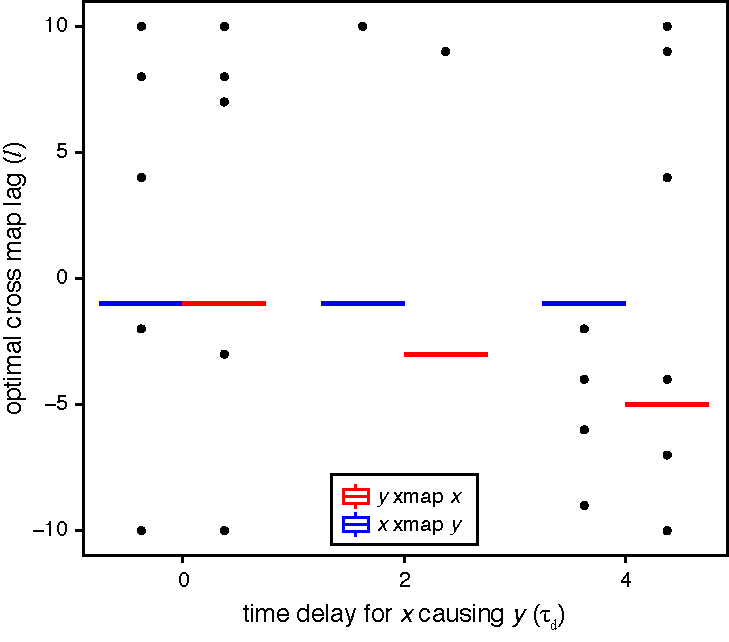
\includegraphics{fig_lag_2sp_delay_rand.pdf}\end{center}
\caption[Robustness of extended CCM in the 2-species logistic model with bidirectional forcing.]{\textbf{Robustness of extended CCM in the 2-species logistic model with bidirectional forcing.}\newline
Boxplots of optimal cross map lag ($l$) are shown for 500 random simulations of the 2-species logistic model with bidirectional causality and with three different time delays, $\tau_d$. Except for a few outliers, the optimal cross map lag when using $x$ to cross map $y$ (blue, ``$x$ xmap $y$'') is -1, as would be expected, because $x$ responds to $y$ within a single time step. In the opposite direction, a larger time delay ($\tau_d$) in the effect of $x$ on $y$ results in larger negative values for the optimal cross map lag when using $y$ to cross map $x$ (red, ``$y$ xmap $x$'')}
\label{fig_lag_2sp_delay_rand}
\end{figure}

We generalize the simple model system consisting of 2 coupled logistic difference equations as follows:
\begin{align}
\label{eqn_2sp_delay_rand}
\begin{split}
x(t+1) &= x(t) \left[R_x - R_x x(t) - A_{xy} y(t)\right]\\
y(t+1) &= y(t) \left[R_y - R_y y(t) - A_{yx} x(t-\tau_d)\right]
\end{split}
\end{align}

where $\tau_d$ is the time delay for the effect of $x$ on $y$. For each simulation run, we sample a new fixed value for the growth rates $R_x$ and $R_y$ from the uniform distribution $(3.7, 3.9)$, as well as new values for the interaction coefficients $A_{xy}$ and $A_{yx}$ from the uniform distribution $(0.05, 0.1)$. In addition each simulation is initialized with random starting points with $x(1)$ and $y(1)$ drawn from the uniform distribution $(0.01, 0.99)$, and run for 3000 time steps. For each of the different values for the time delay: $\tau_d = 0$, $\tau_d = 2$, and $\tau_d = 4$, we ran a total of 500 simulations (when populations reached negative values or increased beyond carrying capacity, we sampled new coefficients and re-ran the simulation). Using extended CCM, we analyze each simulation using $E = 2$, $\tau = 1$, selecting a random library of 200 vectors over time points 101-2000, and computing cross map skill for time points 2001-3000.

The results are depicted in Figure \ref{fig_lag_2sp_delay_rand}, with boxplots for the value of the cross map lag ($l$) that gives the highest cross map skill ($\rho$). Because nearly all simulations had identical values for the optimal cross map lag ($l$), the boxplots are depicted as straight lines with just a few outliers. As expected, ``$y$ xmap $x$'' (red), depicting the causal effect of $y$ on $x$ has an optimal cross map lag of $l = -1$, because $y$ affects $x$ with a lag of 1 time step ($y(t)$ influences $x(t+1)$). Conversely, the optimal cross map lag for ``$x$ xmap $y$'' (blue) changes depending on $\tau_d$; this is also expected since $\tau_d$ describes the time delay in the response of $y$ to $x$. In fact, the optimal cross map lag for ``$x$ xmap $y$'' appears to accurately recover the time delay parameter $\tau_d$: for example, the optimal $l$ is nearly always -3 when $\tau_d = 2$ (meaning $x(t)$ influences $y(t+3)$ and therefore it takes 3 time steps for $y$ to respond to $x$).

\subsection{Two-Species Model System with Synchrony}

\begin{figure}[!ht]
\begin{center}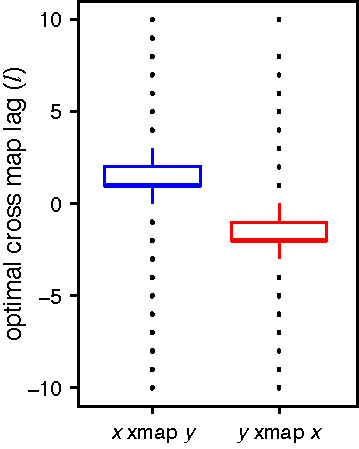
\includegraphics{fig_lag_2sp_synch_rand.pdf}\end{center}
\caption[Robustness of extended CCM in the 2-species logistic model with generalized synchrony.]{\textbf{Robustness of extended CCM in the 2-species logistic model with generalized synchrony.}\newline
Boxplots of optimal cross map lag ($l$) are shown for 500 random simulations of the 2-species logistic model with unidirectional causality producing generalized synchrony. Except for a few outliers, the optimal cross map lag when using $y$ to cross map $x$ (red, ``$y$ xmap $x$'') is negative, and positive in the opposite direction (blue, ``$x$ xmap $y$''). This is expected, because $x$ has a true causal influence on future values of $y$, meaning $y$ is better at cross mapping to past values of $x$; conversely, the lack of an actual effect of $y$ on $x$, but rather ``generalized synchrony'' means that $x$ is better at cross mapping future values of $y$.}
\label{fig_lag_2sp_synch_rand}
\end{figure}

We also generalize the modified form of the above system that produces synchrony with strong forcing from x to y only:

\begin{align}
\label{eqn_2sp_synch_rand}
\begin{split}
x(t+1) &= x(t) \left[R_x - R_x x(t)\right]\\
y(t+1) &= y(t) \left[R_y - R_y y(t) - A_{yx} x(t)\right]
\end{split}
\end{align}

For each simulation, $R_x$ is sampled from the uniform distribution $(3.7, 3.9)$, $R_y$ is sampled from the uniform distribution $(2.5, 3.2)$, and $A_{yx}$ is sampled from the uniform distribution $(0.7, 0.9)$. As above, the system is initialized with random starting points with $x(1)$ and $y(1)$ drawn from the uniform distribution $(0.01, 0.99)$, and run for 3000 time steps. We ran a total of 500 simulations (when populations reached negative values or increased beyond carrying capacity, we sampled new coefficients and re-ran the simulation). Using extended CCM, we analyze each simulation using $E = 2$, $\tau = 1$, selecting a random library of 200 vectors over time points 101-2000, and computing cross map skill for time points 2001-3000.

Results for the ``generalized synchrony'' model are shown in Figure \ref{fig_lag_2sp_synch_rand}, with boxplots showing the value of the cross map lag ($l$) that gives the highest cross map skill ($\rho$). Again, we see that the optimal cross map lag ($l$) is generally negative in the direction of true causality (red, ``$y$ xmap $x$'') and positive in the direction of synchrony (blue, ``$x$ xmap $y$''). 

\subsection{Four-Species Model System}

To test the robustness of extended CCM in distinguishing between direct and indirect causality, we generalize the 4-species model system with a transitive causal chain:

\begin{align}
\label{eqn_4sp_transitive_rand}
\begin{split}
y_1(t+1) &= y_1(t) \left[R_1 - R_1 y_1(t)\right]\\
y_2(t+1) &= y_2(t) \left[R_2 - A_{21} y_1(t) - R_2 y_2(t)\right]\\
y_3(t+1) &= y_3(t) \left[R_3 - A_{32} y_2(t) - R_3 y_3(t)\right]\\
y_4(t+1) &= y_4(t) \left[R_4 - A_{43} y_3(t) - R_4 y_4(t)\right]
\end{split}
\end{align}

For each simulation, the growth parameters are sampled as follows: $R_1$ is drawn from the uniform distribution $(3.8, 4.0)$, $R_2$ and $R_3$ are both drawn from the uniform distribution $(3.5, 3.7)$, and $R_4$ is drawn from the uniform distribution $(3.7, 3.9)$. The interaction parameters $A_{21}$, $A_{32}$, and $A_{43}$ are all drawn from the uniform distribution $(0.3, 0.5)$. As above, the system is initialized with random starting points with each $y_i(1)$ drawn from the uniform distribution $(0.01, 0.99)$, and run for 3000 time steps. We ran a total of 500 simulations (when populations reached negative values or increased beyond carrying capacity, we sampled new coefficients and re-ran the simulation). Using extended CCM, we analyze each simulation using $E = 4$, $\tau = 1$, selecting a random library of 200 vectors over time points 101-2000, and computing cross map skill for time points 2001-3000.

\begin{figure}[!ht]
\begin{center}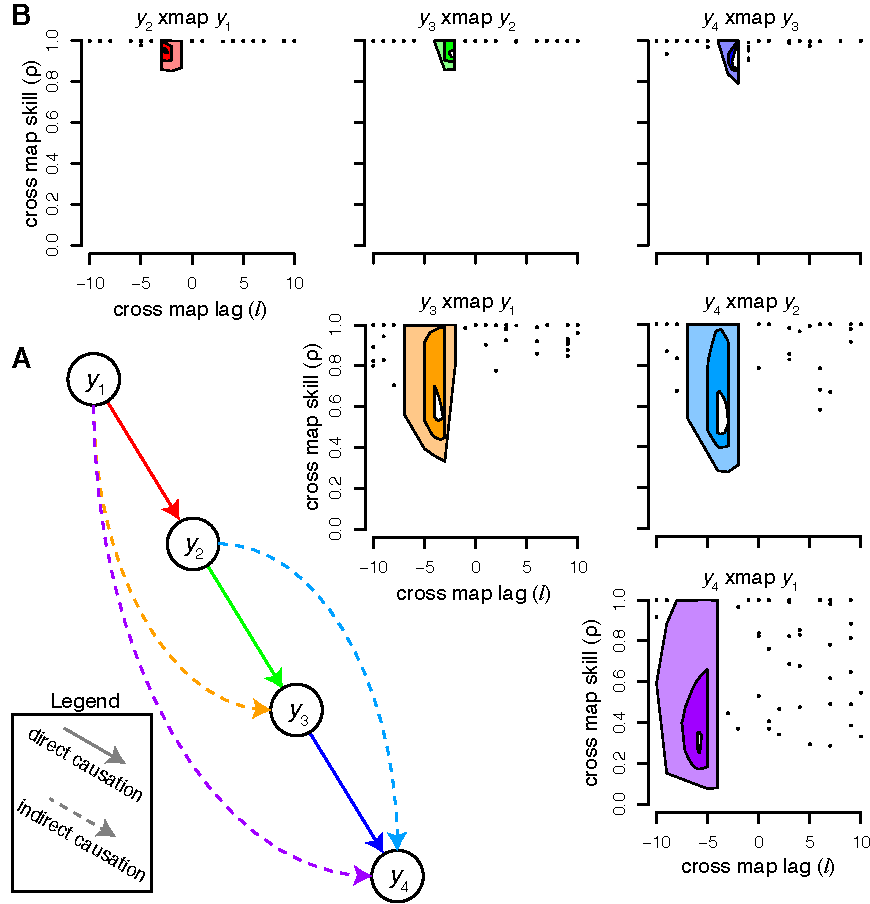
\includegraphics[scale = 0.9]{fig_lag_4sp_transitive_rand.pdf}\end{center}
\label{fig_lag_4sp_transitive_rand}
\caption[Robustness of extended CCM for distinguishing direct and indirect causality in a transitive causal chain.]{\textbf{Robustness of extended CCM for distinguishing direct and indirect causality in a transitive causal chain.}\newline
(A) In this system, $y_1$ causes $y_2$ causes $y_3$ causes $y_4$ such that indirect causation from $y_1$ to $y_3$, $y_2$ to $y_4$, and $y_1$ to $y_4$ occurs. (B) Bagplots show the optimal cross map lag ($l$) and corresponding cross map skill ($\rho$) for 500 random simulations of this system. The white central area depicts the 95\% confidence interval for the median value, while the darker colored region is the ``bag'' containing the central 50\% of points (i.e., similar to an interquartile range), and the lighter colored region is the loop with area 3 times the size of the bag, as described in \cite{Rousseeuw_1999}. The direct links (top row) are strongest with the highest cross map skill and the most immediate effects ($l \sim -2$), while the indirect links separated by one node (middle row) have moderate cross map skill and somewhat delayed effects ($l \sim -4$), and the indirect link from $y_1$ to $y_4$ (bottom row) is the weakest and with the longest time delay ($l \sim -6$)}
\end{figure}

Results for this analysis are shown in Figure \ref{fig_lag_4sp_transitive_rand}, with bagplots \cite{Rousseeuw_1999} depicting the bivariate boxplots for the optimal cross map lags $l$) and corresponding cross map skill ($\rho$). As in Figure \ref{fig_lag_4sp_transitive}, the top row of panel b shows that the optimal cross map lags are close to 0 and show high cross map skill, as would be expected for these direct interactions. In contrast, the indirect interactions generally have optimal cross map lags that are more negative, and lower cross map skill, with the most indirect interaction (from $y_1$ to $y_4$, identified using $y_4$ xmap $y_1$) showing the most negative cross map lag and the lowest cross map skill. We note that the variance in cross map skill is quite high, indicating that it may not be as useful in separating direct from indirect interactions in real systems, whereas cross map lag shows clearer separation.

\section{Acknowledgments}
This research is supported by Department of Defense, Strategic Environment Research and Development Program RC-2509 (GS, ERD, HY), Lenfest Ocean Program \#00028335 (GS), National Science Foundation Grant No. DEB-1020372 (GS, HY), NSF-NOAA Comparative Analysis of Marine Ecosystem Organization (CAMEO) program Grant NA08OAR4320894/CAMEO (GS), National Science Foundation Graduate Research Fellowships (ERD, HY), Environmental Protection Agency Science to Achieve Results Fellowship (ERD), European Research Council Advanced Grant (LJG, awarded to Jordi Bascompte), the Sugihara Family Trust (GS), the Deutsche Bank-Jameson Complexity Studies Fund (GS), and the McQuown Chair in Natural Science (GS).

Chapter \ref{chap_ccm_time_delays}, in full, is a reprint of material published by Nature Publishing Group as: Hao Ye, Ethan R. Deyle, Luis J. Gilarranz, and George Sugihara. (2015) Distinguishing time-delayed causal interactions using convergent cross mapping. \emph{Scientific Reports} 5: 14750. The dissertation author was the primary investigator and author of this paper.
\chapter{Complexity is Not a Curse: Leveraging Information in Interconnected Systems}
\label{chap_multiembed}

\section{Abstract}
Many real-world systems exhibit complex behaviors that result from interacting coupled components. This interconnectedness is often perceived as an obstacle for modeling, because of the difficulties in fitting mathematical equations with large numbers of variables. We present an alternative approach, Multiview Embedding (MVE), based on the concept of reconstructing system dynamics empirically from time series data. MVE uses the fact that each variable records not just its own behavior, but also that of interacting components, such that information is actually duplicated across different variables. By combining different models of the same system, forecasts can be dramatically improved, as we demonstrate for three model systems and a mesocosm experiment. Thus, MVE represents a new approach for information extraction, turning complexity into an advantage.

\section{Introduction}
A major challenge is to understand and predict complex systems, such as ecosystems, financial networks, and medicine. This is because much of the behavior in these systems is determined by interacting components, and even small perturbations of one variable can produce unexpected or catastrophic results on other parts of the system \cite{Scheffer_2001}. The study of these systems becomes especially difficult as complexity increases: more variables means a much greater increase in the number of possible interactions (the ``curse of dimensionality''; \cite{Donoho_2000, Fulton_2010}. Nevertheless, the ability to forecast these complex systems remains highly desirable, and would be of great utility in enabling targeted interventions or preemptive management actions to moderate the impacts of abrupt shifts \cite{Hill_2007, Doak_2008}.

Although traditional mathematical models have been applied to complex systems, they often show great sensitivity to parameters, model structure, and fitting routines \cite{Wood_1999}. Moreover, model complexity often exceeds what can be uniquely determined by the data. The alternative, strategically expedient, approach of reducing complexity (by e.g., aggregating species into trophic levels or functional groups, decomposing the system into independent components, holding parameters constant) can produce unrealistic behavior, leading to large uncertainties, overconfidence in long-term forecasts, and incorrect stability estimates \cite{Pahl-Wostl_1997, Fulton_2001, Clark_2001, Fulton_2003, Sugihara_2011}.

The identification of important interactions can itself be a challenging problem, with classical methods, such as correlation or Granger causality \cite{Granger_1969} insufficient when applied to systems with dynamic, state-dependent behavior \cite{Sugihara_2012}. Indeed, alternative frameworks that empirically reconstruct system behavior from data (Empirical Dynamic Modeling, EDM), have several advantages over classical approaches when modeling dynamic systems \cite{Perretti_2013, Deyle_2013, Ye_2015}. Here, we develop a new approach within the EDM framework to address the challenges associated with modeling high-dimensional complex systems.

\begin{figure}[!ht]
\begin{center}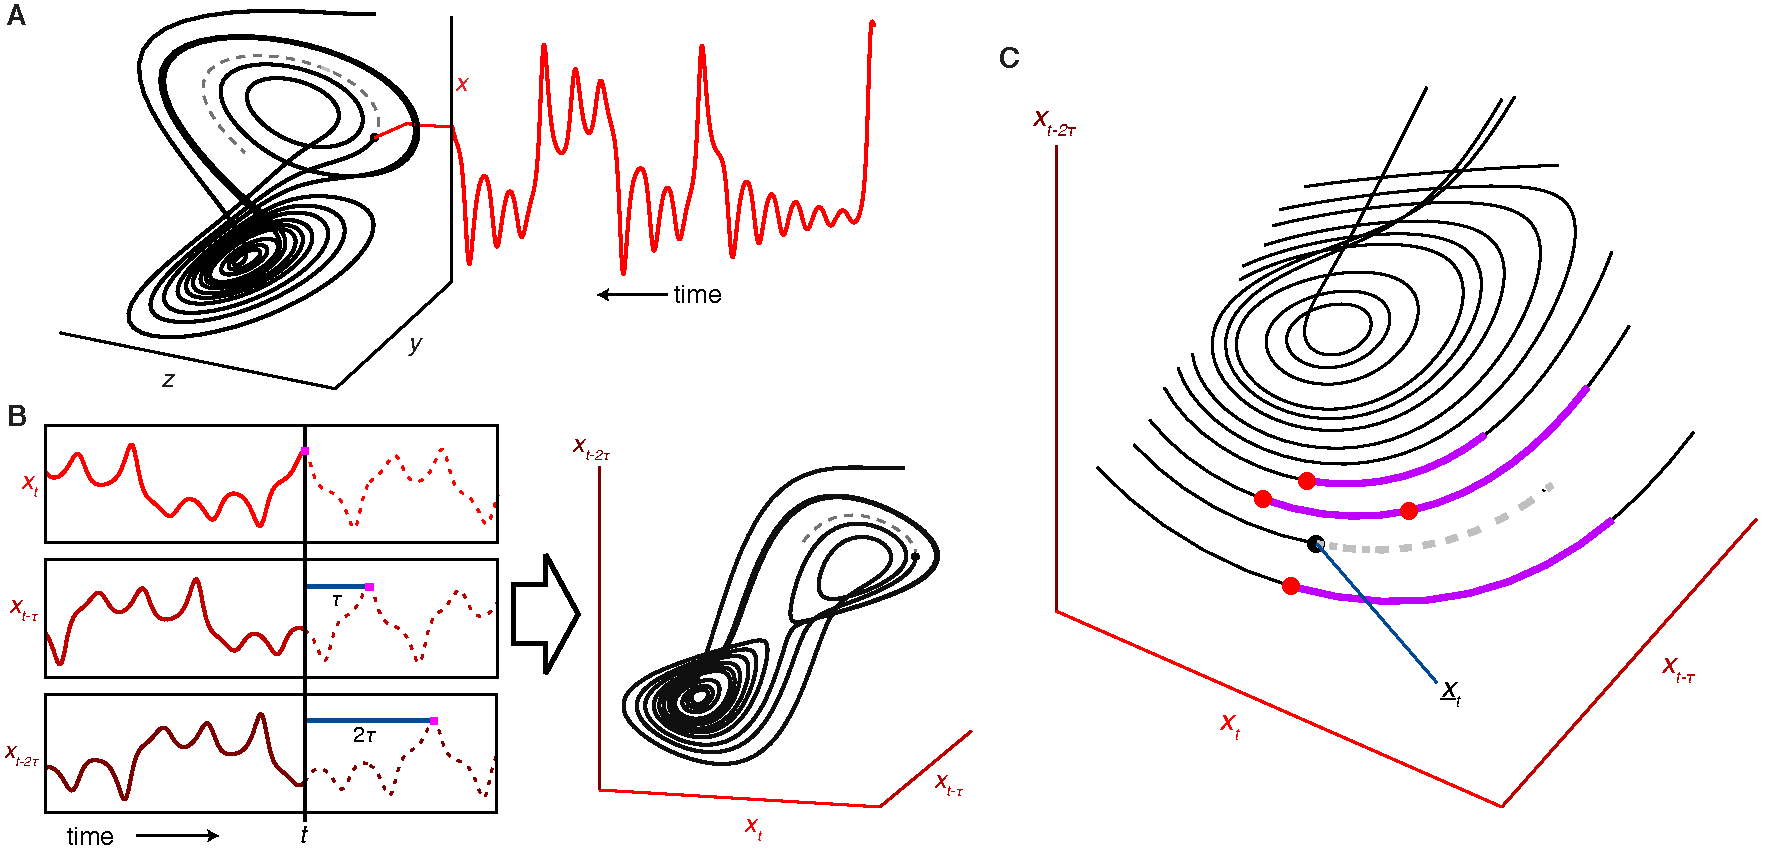
\includegraphics[width=\textwidth]{fig_multiembed_1.pdf}\end{center}
\caption[Attractor reconstruction from a time series.]{\textbf{Attractor reconstruction from a time series.}\newline
(A) Projecting the motion of the canonical Lorenz attractor onto the $x$-axis yields a time series for variable $x$. (B) Successive lags (with time step $\tau$) of the time series $x_t$ are plotted as separate coordinates to form a reconstructed ``shadow'' manifold, which appears similar to the original manifold in panel (A). (C) A magnified view shows nearest neighbor forecasting, whereby the nearest neighbors (red points) to the current observed vector $x_t$ (black point) are used to infer the behavior of the system going forward: the trajectories (purple lines) of the nearest neighbors are averaged to estimate the future behavior (gray dashed line) of $x_t$.}
\label{fig_multiembed_attractor_reconstruction}
\end{figure}

Unlike standard mathematical models, Empirical Dynamic Modeling (EDM) does not use hypothesized or assumed equations, and instead recovers behavior and interactions from the data directly. The essential idea is that time series are observations of the system dynamics (see Fig. \ref{fig_multiembed_attractor_reconstruction}a), which can be reconstructed by projecting successive lags of a single time series as separate coordinates (see Fig. \ref{fig_multiembed_attractor_reconstruction}b; \cite{Crutchfield_1979, Packard_1980, Takens_1981}). Using a sufficient number of lags, the dynamics unfold such that each point corresponds to a unique system state, with nearby points representing similar system states. These reconstructions can then produce forecasts via nearest-neighbor methods (see Fig. \ref{fig_multiembed_attractor_reconstruction}c; \cite{Lorenz_1969, Sugihara_1990}).

As a data-driven approach, EDM models are constrained by the available data: time series of 50 points or longer may be required to uniquely identify system states and nearest neighbors. This can be problematic for datasets that have been sampled for only short periods of time. One potential remedy is to combine data from multiple similar systems into a single composite attractor (``dewdrop regression'', \cite{Hsieh_2008, Clark_2015}) and increase the effective time series length. While reasonable in some situations, the requirement of dynamically equivalent time series is not always met, limiting the application of this technique. Moreover, while such methods directly address estimation error (i.e., an inaccurate model resulting from limited data), they do not address the issue of observational noise.

\begin{figure}[!ht]
\begin{center}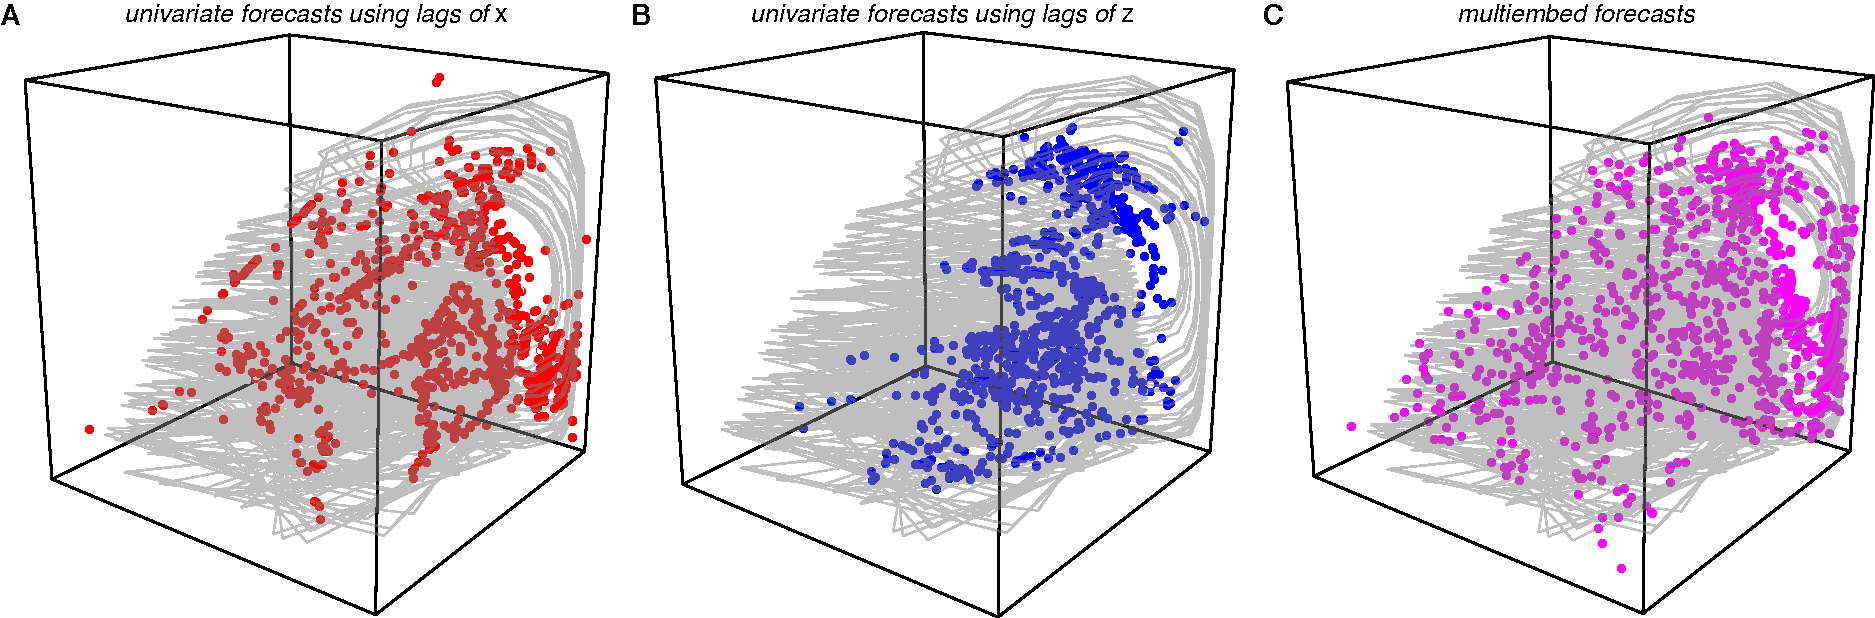
\includegraphics[width=\textwidth]{fig_multiembed_2.pdf}\end{center}
\caption[Information leverage in complex systems.]{\textbf{Information leverage in complex systems.}\newline
(A-B) Univariate reconstructions of the 3-species food chain model give incomplete views of the full system: predictions (solid points) only cover some portions of the original system attractor (grey lines) over the same time period. (C) Combining information from multiple reconstructions, the MVE model has a clearer depiction of the actual dynamics, resulting in predictions that span much more of the original system attractor. The same 1000 points are predicted by each model, based on the same 50 point library (see Methods).}\label{fig_multiembed_information_leverage}
\end{figure}

Here we introduce ``multiview embedding'' (MVE) as an EDM-based solution for modeling complex systems. The idea behind MVE is to exploit the property that time series contain information about causally related components \cite{Sugihara_2012}; as such, different time series from the same system contain redundant information. By combining these time series in different ways, multiple views of the same system can be constructed; together, these multiple then produce a clearer depiction of the dynamics (similar in spirit to stereoscopy where two 2D images form a single 3D image; see Fig. \ref{fig_multiembed_information_leverage}). In fact, because any generic combination of variables and lags is a valid reconstruction \cite{Sauer_1991, Deyle_2011}, the number of such views grows combinatorially with the number of variables, enabling substantial data leverage. Using $l$ lags for each of $n$ variables, the number of reconstructions of dimension $E$ is given by ${n l \choose E} - {n (l-1) \choose E}$\footnote{Note that ${n l \choose E}$ is the number of ways to choose $E$ coordinates from the $n l$ variable $\times$ lag combinations. The correction of ${n (l-1) \choose E}$ accounts for repeated counting (e.g., $\langle x(t), y(t) \rangle$ and $\langle x(t-1), y(t-1) \rangle$ represent the same reconstruction).}; with 10 time series, and $E = l = 3$, nearly 3000 different reconstructions are possible!

\section{Results}

\begin{figure}[!ht]
\begin{center}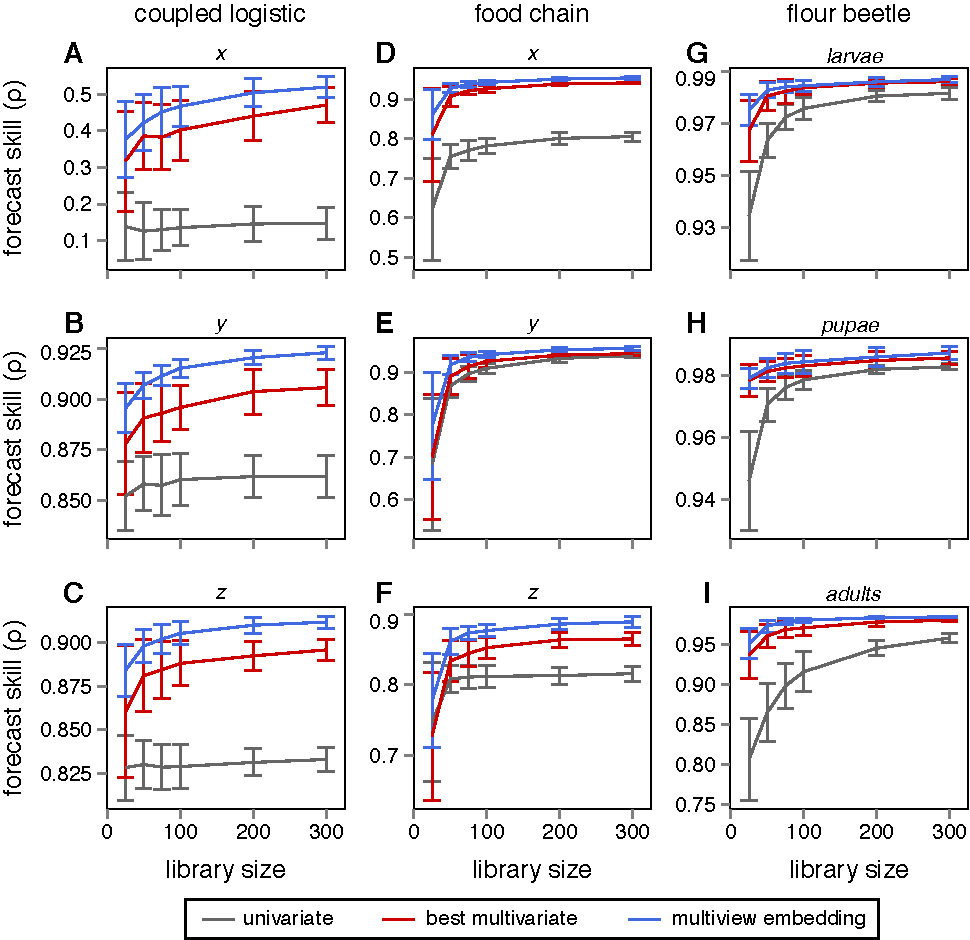
\includegraphics[width=\textwidth]{fig_multiembed_3.pdf}\end{center}
\caption[Comparison of forecast performance for model systems.]{\textbf{Comparison of forecast performance for model systems.}\newline
Multiview embedding produces more accurate forecasts than the best multivariate and univariate methods. (A-C) Forecast skill ($\rho$, correlation between observations and predictions) vs. library size for variables $x$, $y$, and $z$, in the coupled logistic map. Lines indicate average values over 100 randomly sampled libraries (see Methods) and error bars denote $\pm 1$ standard deviations. (D-F) Same as A-C, but for the 3-species food chain model. (G-I) Same as A-C, but for the flour beetle model.}
\label{fig_multiembed_model_results}
\end{figure}

To demonstrate multiview embedding (MVE), we implement a model-\linebreak averaging approach. First, we generate all possible reconstructions, computing the performance of each based on an in-sample training set (see Methods). Then, an MVE model is defined as the average of the top $25\%$ of these reconstructions and tested on an out-of-sample test set. Figure \ref{fig_multiembed_model_results} compares the performance of this MVE model with two commonly-used EDM methods: a ``univariate'' model, using only lags of the variable being forecast, and a ``best multivariate'' model, using the single reconstruction with the highest in-sample performance. For the three ecosystem models \cite{Hastings_1991, Dennis_2001}, MVE has the most predictive power (a measure of information gained; see Methods) as well as the highest accuracy ($\rho$, correlation between observations and predictions), and the lowest error (mean absolute error, MAE; and root mean square error, RMSE; see Figs. \ref{fig_multiembed_ed_1}-\ref{fig_multiembed_ed_3}).

\begin{figure}[!ht]
\begin{center}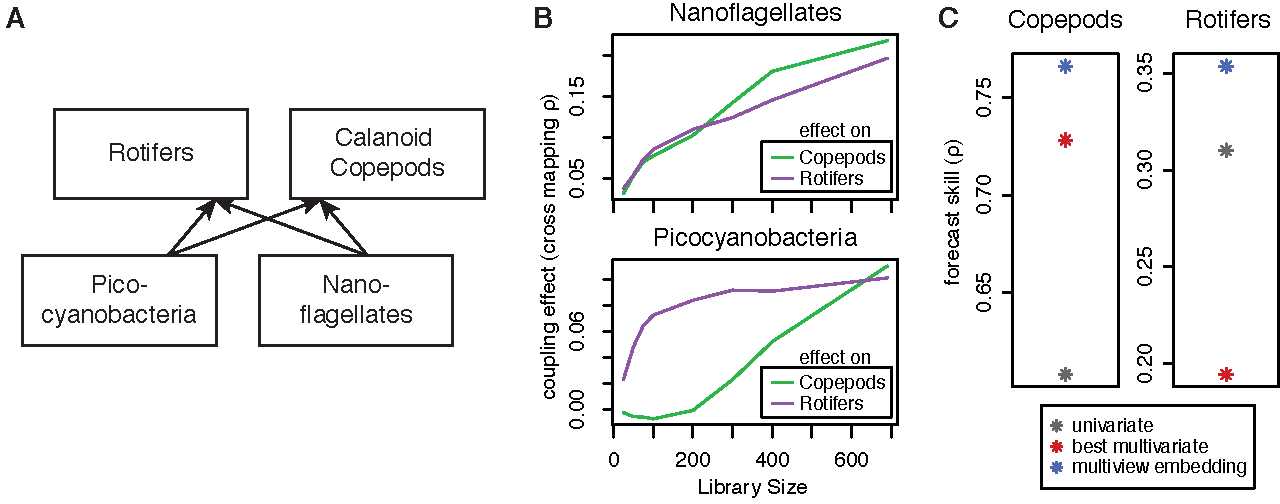
\includegraphics[width=\textwidth]{fig_multiembed_4.pdf}\end{center}
\caption[Analysis of the long-term mesocosm experiment.]{\textbf{Analysis of the long-term mesocosm experiment.}\newline
Panel (A) shows a portion of the food web. (B) Cross mapping between the grazers (calanoid copepods and rotifers) and the two prey items (nanoflagellates and picocyanobacteria) indicating causal influence of the prey items on the grazers. (C) Forecast accuracy ($\rho$) is higher for multiview embedding than for the univariate or best multivariate methods.}
\label{fig_multiembed_mesocosm_results}
\end{figure}

We next apply MVE to time series from a long-term mesocosm experiment \cite{Heerkloss_1998, Beninca_2009}. Here, convergent cross mapping \cite{Sugihara_2012} verifies that the two grazers (rotifers and calanoid copepods) are causally influenced by their prey (nanoflagellates and picocyanobacteria) (see Fig. \ref{fig_multiembed_mesocosm_results}ab). Thus, we produce models to forecast grazer abundances that include both prey time series as possible coordinates. Again comparing MVE to the ``univariate'' and ``best multivariate'' EDM models, the overall results are similar to those for the simulated ecosystems (see Fig. \ref{fig_multiembed_mesocosm_results}c, Fig. \ref{fig_multiembed_ed_4}), with MVE outperforming both of the other two methods.

\section{Discussion}
Accurate forecasts from a model require identification of the current state and estimation of how the system will evolve from that state. Consequently, predictive skill is diminished when a model does not clearly distinguish between states with divergent trajectories. Although Takens' Theorem and its generalizations suggest that all attractor reconstructions are valid \cite{Takens_1981, Sauer_1991, Deyle_2011}, in practical settings, observation error, limited time series length, and noise amplification mean that reconstructions can differ greatly in predictive skill \cite{Casdagli_1991}.

For example, in the 3-species coupled logistic map, forecasts produced by univariate models are inaccurate, and improve very little with more data (gray lines, Fig. \ref{fig_multiembed_model_results}a-c). This occurs because of the strong nonlinear interactions in this model: future values of a single variable, such as $y$, can depend greatly on the value of other variables ($x$ and $z$). In univariate models that include only lags of $y$, it can be difficult to infer the concurrent values of $x$ and $z$, thereby limiting forecast skill. Because of these limitations of univariate models, increasing the time series length may only result in marginal improvements in performance.

In contrast, multivariate models that include direct observations of the interacting variables can produce more complete depictions of the system dynamics.  The result is better forecasts that also show substantial improvement with increased library size (red lines, Fig. \ref{fig_multiembed_model_results}a-c). Because there are many ways to form multivariate reconstructions, we perform model selection on the in-sample data to choose the reconstruction that gives the highest accuracy. This enables the selection of the most relevant variables and lags for each forecast target. We further note that, unlike the traditional approach of creating a single complex model for the entire system, this model selection approach can select different reconstructions depending on the target variable. In other words, there is no single best model for the system, but a collection of different models for different components of the system.

Surprisingly, the MVE model produces better forecasts than the multivariate approach, even though MVE is essentially an average of different models (only one of which is the ``best'' multivariate model). We hypothesize that the improved performance of MVE is due to a reduced effect of observational error when combining multiple views of the system dynamics. Insofar as different time series variables can be reasonably assumed to have independent observation errors, combining different views of the system will increase precision and produce better forecasts. This is especially important when time series are short, because the reconstructions will be relatively sparse, and the selection of nearest neighbors will be unreliable. 

For example, in both the univariate and multivariate approaches, nearest neighbors are identified by distance in the reconstructed state space. If the data are subject to observation error, then the distance metric will be an uncertain measure of how similar these states actually are. Whereas points are normally weighted based on this distance metric, MVE effectively weights these points based on often it is the nearest neighbor among the best reconstructions. The improved forecasts suggest that this approach is a more reliable measure of whether points represent truly similar analogue states, thus allowing MVE forecasts to outperform single embedding-based models.

We note that noise reduction can also compensate for short time series length. For example, in the flour beetle model (see Fig. \ref{fig_multiembed_model_results}g-i), the dynamics appear to be well explained with the univariate method once time series are long enough ($\sim200$ points). However, in many practical circumstances, time series length is limited, and single reconstructions are not dense enough to counteract the effects of noise. Instead of requiring many neighbors to decrease error, MVE uses different reconstructions. Thus, at the smallest library size (25 points), the performance of MVE is often comparable to that of the best multivariate method with 2-3 times more data, and in many cases surpasses the univariate method even when the latter has 10 times more data.

Although we use a simple ranking and averaging scheme to implement MVE, more sophisticated methods to combine reconstructions (e.g., a weighted average, different ranking depending on system state) could produce further improvements, especially when larger datasets are available or when system-specific knowledge is available (e.g., noise structure, likely causal drivers). An obvious benefit to MVE is that with more time series, a clearer picture of the system dynamics emerges, as each additional variable increases the number of possible reconstructions. Because the number of reconstructions grows combinatorially with the number of variables, we suggest judiciously selecting only the relevant time series variables when applying MVE. As demonstrated here, convergent cross mapping (CCM) \cite{Sugihara_2012} can be used in conjunction with system-specific knowledge to identify the most informative variables for a given forecasting target. CCM is uniquely suited for this task, as it detects the presence of causal interactions using the same empirical framework as MVE.

\section{Conclusions}

The primary advantage of MVE is in leveraging multiple time series observations of a single system. That these time series represent interconnected components is actually a prerequisite for MVE, because it means that dynamical information is duplicated across different variables \cite{Sugihara_2012}. By using the equation-free approach of EDM, this information can then be extracted and re-combined. This approach to rich datasets allows MVE models to mitigate the effect of noisy observations, and is fundamentally different from other noise reduction algorithms.. For example, the Kalman filter \cite{Kalman_1960} assumes that the underlying dynamics are known and that noise is linearly separable, two assumptions that are typically unsuitable for complex systems.

Here, we demonstrate the usage of MVE to improve forecasts; however, MVE has potential benefits in many applications where noise reduction is a challenge, such as signal processing \cite{Carroll_2012} and nonlinear control systems \cite{Ott_1990}. Although the high-dimensionality of complex systems is typically perceived as an obstacle, MVE shows, counterintuitively, that complexity is actually an opportunity for information leverage.

\section{Methods Summary}

We used time series from 3 different models (a coupled logistic map, a 3-species food chain \cite{Hastings_1991}, and a flour beetle model \cite{Dennis_2001}) and data collected from a long-term mesocosm experiment (a plankton community isolated from the Baltic Sea; \cite{Heerkloss_1998, Beninca_2009}). For the model systems, 3000 points were generated with simulated observation error. For the mesocosm data, we sampled segments from the raw data, by using all segments of at least 15 points where the lag between points was 6-8 days, resulting in 17 segments comprising 725 data points. Time series were rescaled to mean = 0 and variance = 1.

For each model system, we generated all 3-dimensional attractor reconstructions, allowing lags of 0, 1, or 2, resulting in 64 unique reconstructions for each system. We applied a similar procedure to 2 subsystems from the mesocosm data, where each subsystem consisted of one of the grazers (rotifers or calanoid copepods) and its two main prey items (picocyanobacteria and nanoflagellates) (see Fig. 4a). We computed in-sample performance on ``library'' segments using simplex projection \cite{Sugihara_1990} and leave-one-out cross-validation to forecast 1 time step ahead. The attractors were then ranked based on $\rho$, the correlation coefficient between observations and predictions. This ranking identified the reconstructions to be used in the ``multivariate'' (best $\rho$) and MVE (top 16 $\rho$) methods when making out-of-sample forecasts.

We measured forecast skill using 4 different metrics: $\rho$, MAE (mean absolute error), RMSE (root mean square error), and predictive power (a measure of information gain \cite{Schneider_1999}). For the ecosystem models, we randomly subsampled 100 contiguous libraries (ranging in size from 25 to 300 vectors) from among the first 1300 points, and producing out-of-sample forecasts for the last 500 points. For the mesocosm data, we used an approximate 4-fold cross-validation scheme, assigning the 17 segments into 4 roughly-equally sized subsets.

\section{Methods}

\subsection{Data Sources}

We used time series generated from 3 different models (described below) and data collected from a long-term mesocosm experiment using a plankton community isolated from the Baltic Sea \cite{Hastings_1991, Dennis_2001, Heerkloss_1998, Beninca_2009}.

\subsection{Ecosystem Models}

\subsubsection{Coupled Logistic Map}

We modeled 3 interacting species using the coupled logistic map:

\begin{equation}
\label{eqn_coupled_map}
\begin{bmatrix}
x_{t+1}\\
y_{t+1}\\
z_{t+1} \end{bmatrix} = \vec{r} \circ 
\begin{bmatrix}
x_t\\
y_t\\
z_t \end{bmatrix} \circ 
\left(
\begin{bmatrix}
1\\
1\\
1 \end{bmatrix}
- A \times 
\begin{bmatrix}
x_t\\
y_t\\
z_t \end{bmatrix}
\right)
\end{equation}
where $\vec{r}$ is a $3 \times 1$ vector, $A$ is a $3 \times 3$ matrix with $A_{i, i} = 1$, and $\circ$ is the Schur product (entrywise product). We used initial conditions $\begin{bmatrix}
x_1\\
y_1\\
z_1 \end{bmatrix} = 
\begin{bmatrix}
0.2\\
0.2\\
0.2 \end{bmatrix}$, $r = \begin{bmatrix}
3.6\\
3.0\\
3.0 \end{bmatrix}$, and $A = \begin{bmatrix}
1 & 0.2 & 0.2\\
0.2 & 1 & -0.2\\
0.2 & -0.2 & 1 \end{bmatrix}$.

\subsubsection{3-species Food Chain}

We modeled a 3-species food chain following \cite{Hastings_1991}:

\begin{equation}
\label{eqn_3sp_food_chain}
\begin{array}{rl}
dx/dt &= x(1-x)-f_1(x)y\\
dy/dt &= f_1(x)y - f_2(y)z - d_1y\\
dz/dt &= f_2(y)z - d_2(z)
\end{array}
\end{equation}

where

\begin{equation*}
f_i(u) = a_i u / \left(1+b_i u \right)
\end{equation*}

We used the parameterization $a_1 = 2.5$, $b_1 = 3.2$, $b_2 = 2.0$, $d_1 = 0.2$, and $d_2 = 0.015$; and initial conditions $x_0 = 0.8$, $y_0 = 0.2$, and $z_0 = 8$.

\subsubsection{Flour Beetle Model}

We modeled 3 life stages (larvae, pupae, and adults) of the flour beetle, \emph{Tribolium castaneum} following \cite{Dennis_2001}:
\begin{equation}
\label{eqn_flour_beetle}
\begin{array}{rl}
L_{t+1} = b A_t \exp{\left(-c_\textrm{el}L_t - c_\text{ea}A_t\right)}\\
P_{t+1} = L_t \left(1 - \mu_l\right)\\
A_{t+1} = P_t \exp{\left(-c_\textrm{pa}A_t\right) + A_t\left(1 - \mu_a\right)}
\end{array}
\end{equation}
parameterization $b = 10.67$, $\mu_l = 0.1955$, $\mu_a = 0.96$, $c_\textrm{el} = 0.01647$, $c_\textrm{ea} = 0.01313$, and $c_\textrm{pa} = 0.35$, which are the maximum-likelihood estimates of the model parameters from real data, but with $c_\textrm{pa}$ adjusted to give chaotic dynamics \cite{Dennis_2001}. Initial conditions were $L_1 = 250$, $P_1 = 5$, and $A_1 = 100$.

\subsubsection{Time Series Generation}

The coupled logistic map and flour beetle model were run forward in time following equations \ref{eqn_coupled_map} and \ref{eqn_flour_beetle}, respectively. The 3-species food chain model was run by solving equation \ref{eqn_3sp_food_chain} using the classical Runge-Kutta method with a time step of 0.01 and downsampling by a factor of 800. For each model, we generated time series with 2000 points, and then simulated observation error by multiplying each time series with i.i.d. white noise drawn from a lognormal distribution with mean = 1 and CV (coefficient of variation) = 0.1. Next, we rescaled each time series to mean = 0 and variance = 1. (This ensures that the distance calculations for each attractor reconstruction are not skewed by the choice of coordinates.)

\subsection{Plankton Community}

This experiment has previously been described in numerous publications as an example of chaotic dynamics. We used the raw data from the supplement of \cite{Beninca_2009} and focused on forecasting the abundances of rotifers (mainly \emph{Brachionus plicatilis}) and the calanoid copepod \emph{Eurytemora affinis}. \cite{Beninca_2009} noted that the primary food items of the rotifers and calanoid copepods were picocyanobacteria and nanoflagellates (see Fig. \ref{fig_multiembed_mesocosm_results}a). We used convergent cross mapping \cite{Sugihara_2012} to verify that causal information about the prey abundances were present in the predator abundances (see Fig. \ref{fig_multiembed_mesocosm_results}b). Thus multivariate attractor reconstructions using the prey time series are suitable for forecasting the predators (rotifers and calanoid copepods).

Instead of interpolating the data (which can pollute the dynamics by combining information from multiple sampling times), we instead extracted all possible segments of 15 points or more and where the lag was 6-8 days ($\sim 1$ week). This procedure resulted in 17 segments, comprising 725 data points. Next, we applied the same fourth root transformation of \cite{Beninca_2009} to suppress sharp peaks that distort the attractor reconstruction (especially when searching for nearest neighbors) before applying the scaling procedure described above. Forecast statistics were computed after reversing the transformations.

\subsection{Attractor Reconstruction}

For each system, we generated all possible 3-dimensional attractor reconstructions where each coordinate could be any of the 3 time series variables with a lag of 0, $\tau$, or $2\tau$. Then we kept only the reconstructions where at least one coordinate had no lag, resulting in 64 attractors for each model system. For all models, we used $\tau = 1$. (Note that for the 3-species food chain model, $\tau$ is effectively 8, because we ran the model using a time step of 0.01 and downsampled by 800, and for the mesocosm data $\tau = 1$ corresponds to $\sim 1$ week.)

In the general case with $n$ time series variables, $l$ possible lags for each variable, and embedding dimension $E$, the number of possible attractor reconstructions is given by

\begin{equation*}
{n l \choose E} - {n (l-1) \choose E}
\end{equation*}

where ${n l \choose E}$ is the number of attractors formed by choosing $E$ of the $nl$ possible coordinates, and ${n (l-1) \choose E}$ is the number of ``invalid'' attractors where all $E$ coordinates are chosen from among the $n(l-1)$ possible coordinates with positive (i.e. nonzero) lag.

\subsection{Multiview Embedding}

Using the method of simplex projection \cite{Sugihara_1990} and leave-one-out cross-validation, we computed the performance of each attractor reconstruction when forecasting 1 time step ahead on an in-sample portion of the data, called the library. The attractors were ranked based on $\rho$, the correlation coefficient between observations and predictions. The top attractors were then used to produce forecasts for the out-of sample portion of the data. The multiview embedding forecast is defined to be the arithmetic mean of the forecasts from the top attractors:

\begin{equation*}
\hat{y}_{t+p} = \frac{1}{m} \sum_{i = 1}^{m}{y_{nn_1^i(t)+p}}
\end{equation*}

where $m$ is the number of attractors to average over (16 in this case), $nn_1^{i}(t)$ is the time index of the nearest neighbor in the $i$th attractor at time $t$, and $p = 1$ is the prediction horizon.

Conventional simplex projection \cite{Sugihara_1990} uses $b$ nearest neighbors from a single attractor reconstruction, and each of these neighbors represents a unique historical state. These neighbors are weighted by their distance, which is influenced by observational error, so forecasts can be quite sensitive to noise. However, multiview embedding uses the single nearest neighbor from $m$ attractor reconstructions. As these points potentially represent the same historical state and have different observation errors, averaging over them will give a larger weighting towards the points that are consistently closer to the actual system state, in a manner similar to the weighted average used in simplex projection.

\subsection{Performance Metrics}

Forecast skill was measured using 4 different metrics: $\rho$, the correlation coefficient between observations and predictions; MAE, mean absolute error; RMSE, root mean square error; and predictive power \cite{Schneider_1999}. $\rho$ captures forecast accuracy, how well the predictions line up with observations. Both MAE and RMSE capture forecast error, the ``average'' deviation of predictions from observations. Predictive power is an information-theoretic measure that indicates how much uncertainty in the predicted variable is reduced by forecasts.

For the model data, we sampled 100 libraries from the generated time series by choosing the beginning of each library from the uniform distribution [501, 2001]. (Note that we exclude the first 500 points from each time series, so as to reduce the effect of transient behavior.) Out-of-sample forecasts were then produced for last 500 points of the time series (times 2501-3000). The libraries ranged in size from 25 to 300 vectors ($L \in \{25, 50, 75, 100, 200, 300\}$); thus, there was no overlap between the library and forecasts, because the last possible point in the library is at time 2500 and the first point to be forecast is at time 2501. For the mesocosm data, we used a 4-fold cross-validation scheme where 1/4 of the data was held out of sample and the remaining 3/4 was the ``library''. The forecasts for each quarter of the data were then combined before computing statistics. (Note that although the statistics are computed once over the whole time series, the attractors were ranked separate for each 1/4 of the data, so that all forecasts are out-of-sample.).

\section{Extended Data Figures}

\begin{figure}[!ht]
\begin{center}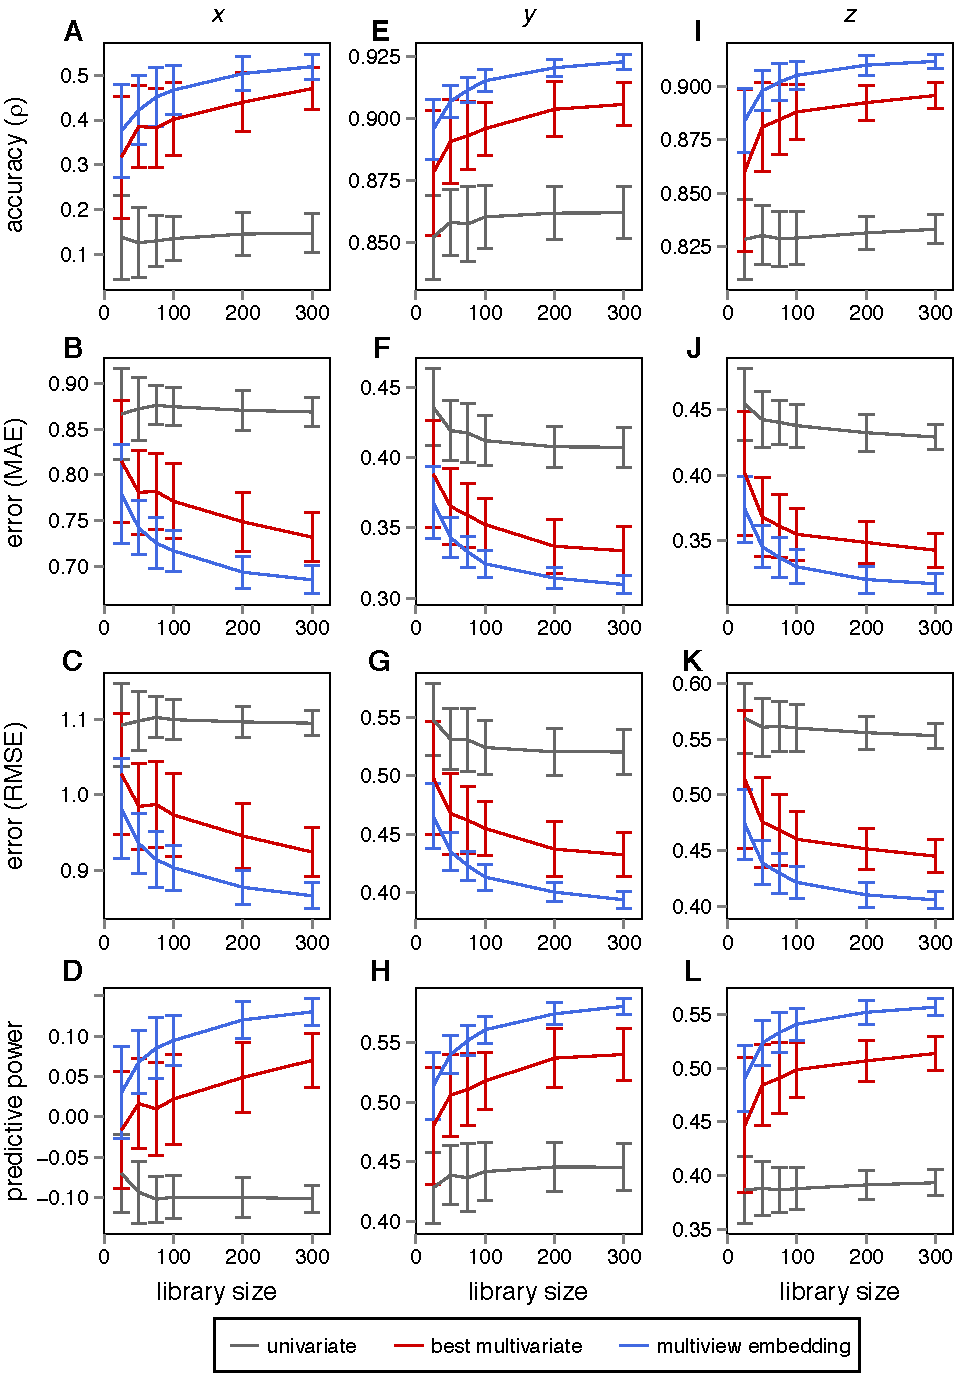
\includegraphics[scale = 0.65]{fig_multiembed_ed_1.pdf}\end{center}
\caption[Comparison of forecast performance for the 3-species coupled logistic map model.]{\textbf{Comparison of forecast performance for the 3-species coupled logistic map model.}\newline
Multiview embedding produces more precise forecasts than the best multivariate and univariate methods for the 3-species coupled logistic map model. (A-D) Forecast accuracy ($\rho$, correlation between observations and predictions), forecast errors (MAE, mean absolute error; RMSE, root mean square error), and predictive power vs. library size for variable $x$. Lines indicate average values over 100 randomly sampled libraries (see Methods) and error bars denote $\pm 1$ standard deviations. (E-H) Forecast accuracy, forecast errors, and predictive power for variable $y$. (I-L) Forecast accuracy, forecast errors, and predictive power for variable $z$.}
\label{fig_multiembed_ed_1}
\end{figure}

\begin{figure}[!ht]
\begin{center}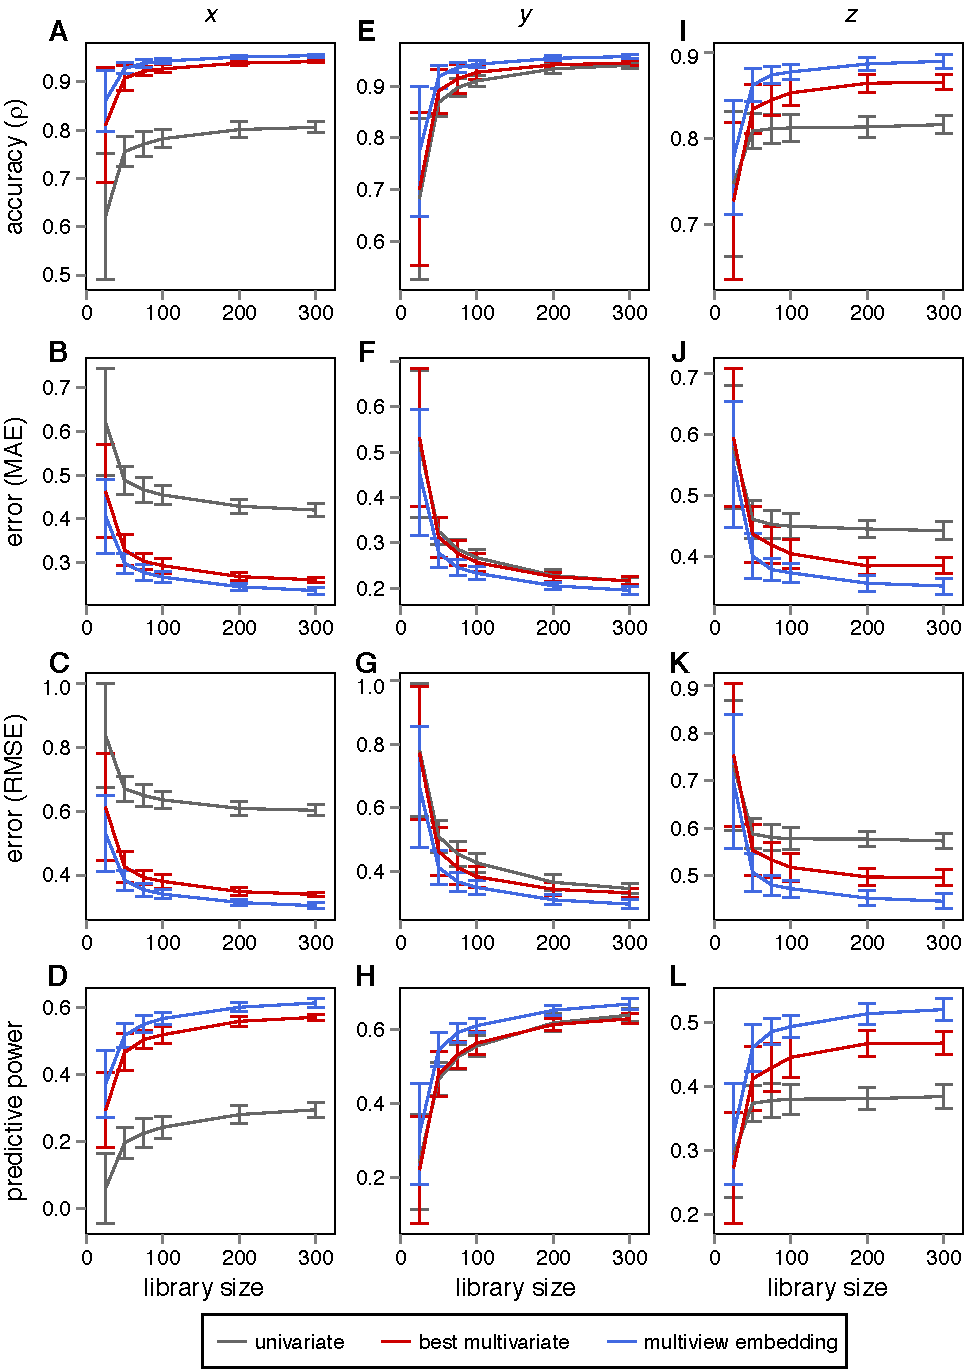
\includegraphics[scale = 0.65]{fig_multiembed_ed_2.pdf}\end{center}
\caption[Comparison of forecast performance for the 3-species food chain model.]{\textbf{Comparison of forecast performance for the 3-species food chain model.}\newline
Multiview embedding produces more precise forecasts than the best multivariate and univariate methods for the 3-species food chain model. (A-D) Forecast accuracy ($\rho$, correlation between observations and predictions), forecast errors (MAE, mean absolute error; RMSE, root mean square error), and predictive power vs. library size for variable $x$. Lines indicate average values over 100 randomly sampled libraries (see Methods) and error bars denote $\pm 1$ standard deviations. (E-H) Forecast accuracy, forecast errors, and predictive power for variable $y$. (I-L) Forecast accuracy, forecast errors, and predictive power for variable $z$.}
\label{fig_multiembed_ed_2}
\end{figure}

\begin{figure}[!ht]
\begin{center}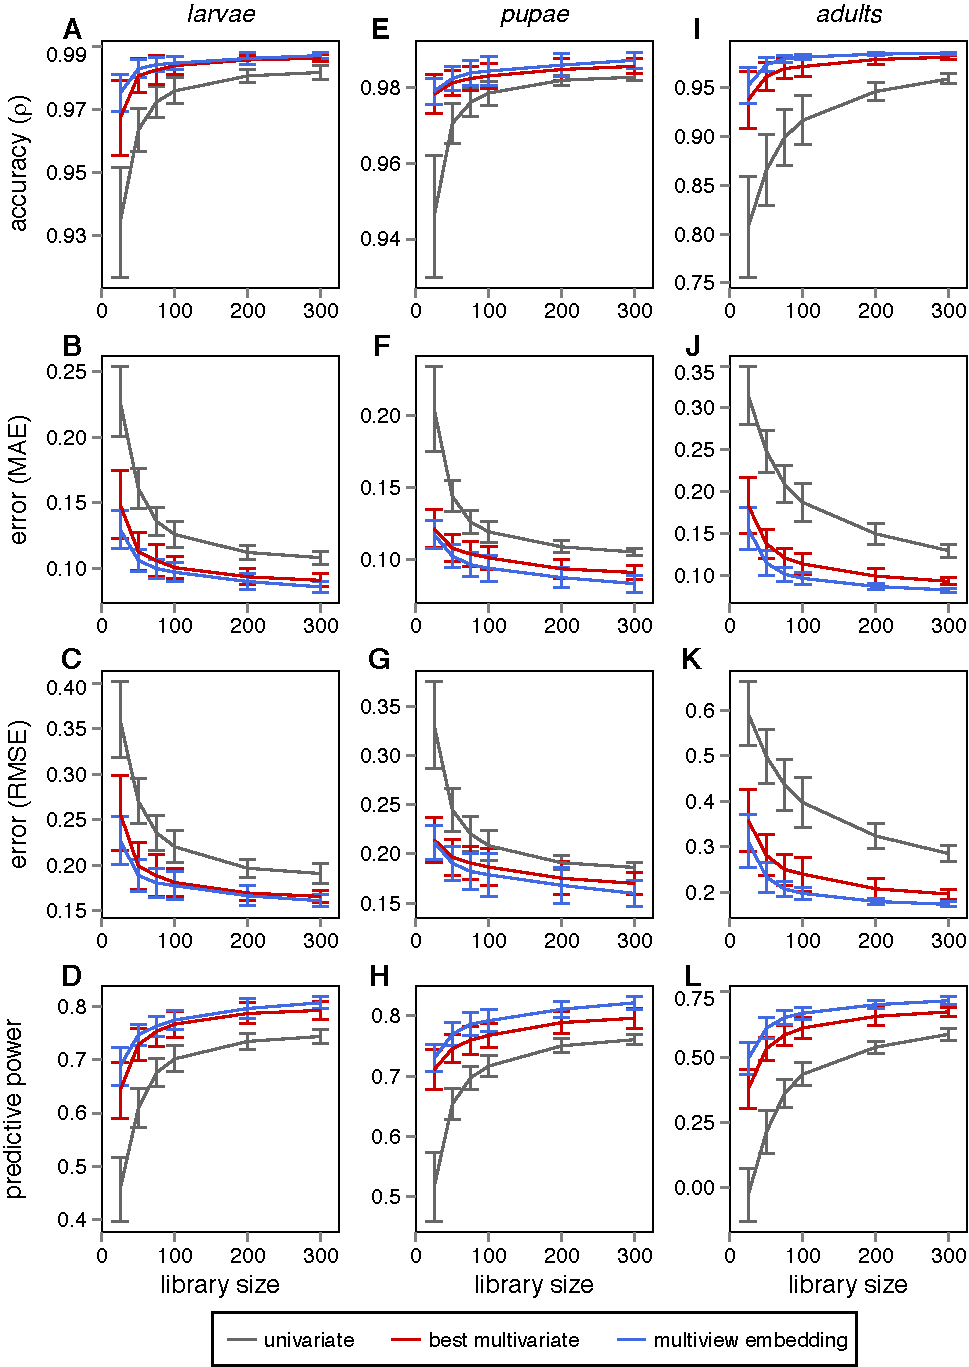
\includegraphics[scale = 0.65]{fig_multiembed_ed_3.pdf}\end{center}
\caption[Comparison of forecast performance for the larvae-pupae-adult flour beetle model.]{\textbf{Comparison of forecast performance for the larvae-pupae-adult flour beetle model.}\newline
Multiview embedding produces more precise forecasts than the best multivariate and univariate methods for the larvae-pupae-adult flour beetle model. (A-D) Forecast accuracy ($\rho$, correlation between observations and predictions), forecast errors (MAE, mean absolute error; RMSE, root mean square error), and predictive power vs. library size for larvae. Lines indicate average values over 100 randomly sampled libraries (see Methods) and error bars denote $\pm 1$ standard deviations. (E-H) Forecast accuracy, forecast errors, and predictive power for pupae. (I-L) Forecast accuracy, forecast errors, and predictive power for adults.}
\label{fig_multiembed_ed_3}
\end{figure}

\begin{figure}[!ht]
\begin{center}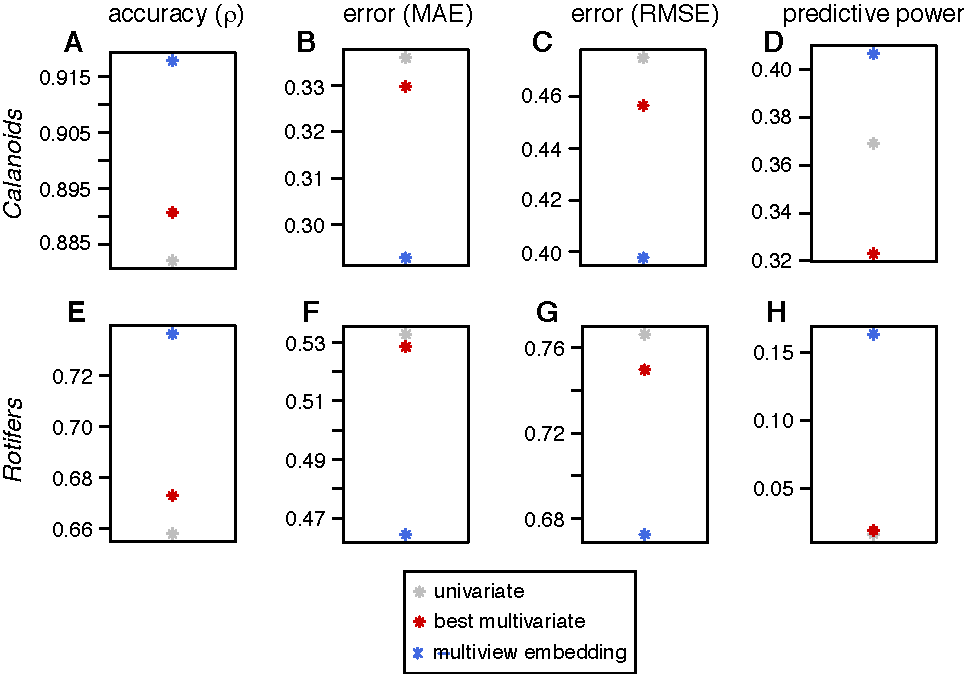
\includegraphics[width=\textwidth]{fig_multiembed_ed_4.pdf}\end{center}
\caption[Comparison of forecast performance for the long-term mesocosm experiment.]{\textbf{Comparison of forecast performance for the long-term mesocosm experiment.}\newline
Multiview embedding produces more precise forecasts than the best multivariate and univariate methods. (A-D) Forecast accuracy ($\rho$, correlation between observations and predictions), forecast errors (MAE, mean absolute error; RMSE, root mean square error), and predictive power when predicting calanoid copepods. (E-H) Forecast accuracy, forecast errors, and predictive power when predicting rotifers.}
\label{fig_multiembed_ed_4}
\end{figure}

\section{Acknowledgments}
This research is supported by Department of Defense, Strategic Environment Research and Development Program W912HQ-15-C-00 (GS, HY), Lenfest Foundation Award 00028335 (GS), National Science Foundation Grant No. DEB-1020372 (GS, HY), NSF-NOAA Comparative Analysis of Marine Ecosystem Organization (CAMEO) program Grant NA08OAR4320894/CAMEO (GS), McQuown Natural Science Research and Education Fund F-2619 (HY), National Science Foundation Graduate Research Fellowships (HY), the Sugihara Family Trust (GS), the Deutsche Bank-Jameson Complexity Studies Fund (GS), and the McQuown Chair in Natural Science (GS).

Chapter \ref{chap_multiembed}, in full, is material prepared for submission: Hao Ye and George Sugihara. Complexity is not a curse: leveraging information in interconnected systems. The dissertation author was the primary investigator and author of this paper.

\appendix
\chapter{rEDM: A Package for Empirical Dynamic Modeling Based on Attractor Reconstruction}
\label{chap_redm_package}

\definecolor{code_bg}{rgb}{0.96, 0.96, 0.96}
\lstset{language = R, upquote = true, backgroundcolor = \color{code_bg}, basewidth = 0.5em}
\lstset{basicstyle = \small\ttfamily, breaklines = true, showspaces = false, showstringspaces = false}

\section{Abstract}
Empirical dynamic modeling (EDM) is an emerging non-parametric framework for modeling nonlinear dynamic systems. In an ecological context, EDM has numerous applications, including forecasting population abundances, unraveling species interactions, and identifying causal drivers. In contrast to the conventional approach of fitting assumed model equations to data, EDM relies on the fact that ecosystems have dynamics that allows us to reconstruct attractors directly from time series. This approach (with minimal assumptions) makes EDM particularly suitable for studying ecosystems, which exhibit non-equilibrium dynamics (problematic for models that typically assume stable equilibria) and state-dependent behavior (interactions that change with system state). This guide is designed to introduce both the theory behind EDM, as well as providing practical examples for using the rEDM software package.

\section{The rEDM package}

\subsection{Installation}
rEDM is an Rcpp package, and contains both C++ and R code. Because the C++ code needs to be compiled prior to usage, there are several different options for obtaining and installing the rEDM package, depending on preference.

\subsubsection{Binary Version}
The precompiled binary version is suitable for mot users and can be downloaded from Github \href{https://github.com/ha0ye/rEDM-binary}{here}. The latest version is 0.2.6 as of August 9, 2015. Clicking on the ``view the full file'' link will initiate a downlaod of the .tgz or .zip file, which can be saved to any desired location. Note that R expects a single package file, so the downloaded archive should not be unpacked into a folder.

To install the downloaded package, the standard R command (\lstinline{install.packages}) as below, replacing \lstinline{***} with the name of the package file. (You will need to either give the complete path, or put the package file in R's current working directory.)

\begin{lstlisting}
install.packages("***", type = "source", repos = NULL)
\end{lstlisting}

Note that the Rcpp package (versions 0.11.5 and higher) must be installed first.

\subsubsection{Source Code Version}
The raw source can be downloaded from Github \href{https://github.com/ha0ye/rEDM}{here}. The package can then be built and installed following the normal procedures.

The source code is managed using Git for version control and includes an RStudio project file, so it can be cloned and built from within RStudio as well.

Finally, the package can also be installed using functions from the \emph{devtools} package:

\begin{lstlisting}
library(devtools)
install_github("ha0ye/rEDM")
\end{lstlisting}

Note that the latter two methods require the Git software to be installed. All methods here require a C++11 compiler, in addition to the Rcpp package. Installation from source has been tested using both Rtools 3.1 for Windows and XCode 5.0+ for Macintosh 10.9+.

\section{Background}

\subsection{Time Series as Observations of a Dynamic System}

The essential concept behind Empirical Dynamic Modeling (EDM) is that time series can be viewed as projections of the behavior of a dynamic system. This framework requires only a few modest assumptions:
\begin{itemize}
\item The system state can be described as a single point in a high-dimensional space. Axes can be thought of as fundamental state variables, such as population abundances, resources, or environmental properties a la the Hutchinson Niche \cite{Hutchinson_1957}.
\item The system state changes through time following some deterministic rules. In other words, the behavior is not completely random.
\end{itemize}

Projecting the system state to an axis then gives the value of the corresponding state variable, and sequential projections over time produce a time series. Different time series observed from the system can capture different state variables, but are more generally, some function of the system state and may convolve several different state variables.

\begin{figure}[!ht]
\begin{center}\includegraphics[width=\maxwidth{\textwidth}]{fig_redm_1.pdf}\end{center}
\caption[Time series from a dynamic system.]{\textbf{Time series from a dynamic system.}\newline
Projecting the motion of the canonical Lorenz attractor onto the $x$-axis yields a time series for variable $x$.}
\label{fig_redm_1}
\end{figure}

\subsection{Attractor Reconstruction / Takens' Theorem}

To reproduce this fundamental, geometric view of the system, one might suppose that time series of all the state variables are required. However, Takens' Theorem \cite{Takens_1981} states that a mathematically equivalent reconstruction can be created by substituting lags of a time series for the unknown or unobserved variables.

In other words, instead of representing a system state as being composed of multiple different state variables, we instead use a lagged-coordinate embedding:
$ \vec{x}_t = \langle x_t, x_{t-\tau}, \dots, x_{t-(E-1)\tau} \rangle $

\begin{figure}[!ht]
\begin{center}\includegraphics[width=\maxwidth{\textwidth}]{fig_redm_2.pdf}\end{center}
\caption[Attractor reconstruction from a time series.]{\textbf{Attractor reconstruction from a time series.}\newline
Successive lags (with time step $\tau$) of the time series $x_t$ are plotted as separate coordinates to form a reconstructed ``shadow'' manifold, which appears similar to the original manifold in Figure \ref{fig_redm_1}.}
\end{figure}

If sufficient lags are used, the reconstruction preserves essential mathematical properties of the original system. For instance, the points will map one-to-one to actual system states, and nearest neighbors in the reconstruction correspond to similar system states and behave similarly in the near future. 

\subsection{Nearest Neighbor Forecasting using Simplex Projection}

One application of the reconstructed attractor is prediction. This can be accomplished using nearest neighbor forecasting methods, because of the similar behavior of nearby points in the reconstruction. One such method is \emph{simplex projection} \cite{Sugihara_1990}. Simplex Projection is implemented in rEDM as the function \lstinline{simplex}, and can be used both for prediction or to identify the optimal embedding dimension by quantifying the forecast skill of reconstructions with different dimensionality.

\subsubsection{Example}

First, we load the data and look at the format. Because this dataset is part of the rEDM package, we need to first load the package into R, before we have access to its datasets and functions.

\begin{lstlisting}
library(rEDM)
data(tentmap_1d)
head(tentmap_1d)
\end{lstlisting}

\begin{lstlisting}[backgroundcolor=\color{white}, commentstyle=\ttfamily]
## [1] -0.0992003 -0.6012986  0.7998003 -0.7944096  0.7979992 -0.8195405
\end{lstlisting}

We can see that the data consists of just a single vector, containing the raw data (first-differences from a tentmap). Because the \lstinline{simplex} function can accept a single vector as the input time series, we don't need further processing of the data. Furthermore, because the data come from a discrete-time model, we can let many of the parameters be default values (e.g., $\tau = 1$, $\text{tp} = 1$). The default values for the embedding dimension, $E$, range from $1$ to $10$, and so the output will allow us to determine which embedding dimension best unfolds the attractor.

We need to specify what portions of the data to use for constructing the simplex projection model, and what portions to use for testing the forecast skill. By default, `simplex` will use leave-one-out cross-validation over the entire time series, but because the data contain no observational noise, and are particularly long, we'd like to be more conservative.

\begin{lstlisting}
lib <- c(1, 100)
pred <- c(201, 500)
\end{lstlisting}

This will use the first 100 points (time = 1 to 100) in the time series as the ``library'' to construct the model, and 300 points (time = 201 to 500) as the ``prediction set'' to test the model.

\emph{Note that if the code detects any overlap in the lib and pred, it will enable leave-one-out cross-validation and return a warning message.}

\begin{lstlisting}
ts <- tentmap_1d
simplex_output <- simplex(ts, lib, pred)
\end{lstlisting}

The results are a simple data.frame with columns for each of the model parameters and forecast statistics, and rows for each run of the model. In this case, there is one run for each value of $E$, so we can simply plot $E$ against $\rho$, the correlation between observed and predicted values:

\begin{lstlisting}
par(mar = c(4,4,1,1), mgp = c(2.5, 1, 0))
plot(simplex_output$E, simplex_output$rho, type = "l", xlab = "Embedding Dimension (E)", ylab = "Forecast Skill (rho)")
\end{lstlisting}

\begin{figure}[!ht]
\begin{center}\includegraphics[width=\maxwidth{\textwidth}]{fig_redm_3.pdf}\end{center}
\caption[Identifying optimal embedding dimension using simplex projection.]{\textbf{Identifying optimal embedding dimension using simplex projection.}\newline
Plotting forecast skill ($\rho$) vs. embedding dimension ($E$) for the first-differenced tent map time series, the optimal embedding dimension is 2.}
\end{figure}

\subsection{Prediction Decay}

An important property of deterministic chaos is that nearby trajectories eventually diverge over time (the so-called ``butterfly effect''). This means that prediction is primarily limited to short-term forecasts, because over the long-term, the system state may be viewed as essentially random. This property also differentiates nonlinear systems from the equilibrium view, where the system can be expected to settle around a stable point.

\subsubsection{Example}

We can test for this property by adjusting the \lstinline{tp} parameter in the models, which determines how far into the future the model seeks to predict:

\begin{lstlisting}
simplex_output <- simplex(ts, lib, pred, E = 2, tp = 1:10)
\end{lstlisting}

Here, we can simply plot tp against $\rho$ to see how forecast accuracy changes as we predict further and further into the future:

\begin{lstlisting}
par(mar = c(4,4,1,1))
plot(simplex_output$tp, simplex_output$rho, type = "l", xlab = "Time to Prediction (tp)", ylab = "Forecast Skill (rho)")
\end{lstlisting}

\begin{figure}[!ht]
\begin{center}\includegraphics[width=\maxwidth{\textwidth}]{fig_redm_4.pdf}\end{center}
\caption[Identifying prediction decay using simplex projection.]{\textbf{Identifying prediction decay using simplex projection.}\newline
Plotting forecast skill ($\rho$) vs. time to prediction (tp) for the first-differenced tent map time series, predictability clearly declines with increasing forecast horizons.}
\end{figure}

\subsection{Identifying Nonlinearity}

One concern is that many time series may show predictability even if they are purely stochastic, because they behave similarly to autocorrelated red noise. Luckily, there are additional tests that can be done to distinguish between red noise and deterministic behavior, by quantifying the degree of "nonlinearity" in the data.

Here, we use the \emph{S-map} forecasting method, that is based on fitting local linear maps for prediction instead of the nearest-neighbor interpolation of simplex projection \cite{Sugihara_1994}. In addition to the parameters for simplex projection, S-map also contains a nonlinear tuning parameter, $\theta$ that affects the weights associated with individual points when fitting the local linear map. When $\theta = 0$, all weights are equal, and the S-map is identical to an autoregressive model; values of $\theta$ above $0$ give greater weight to nearby points in the state space, thereby accommodating nonlinear behavior by allowing the local linear map to vary in state-space. For autoregressive red noise, the linear model should perform better, because the S-map model can reduce observation error by averaging over many points instead of just the most nearby points.

Thus, varying $\theta$ allows us to compare equivalent linear and nonlinear models as a test for nonlinear dynamics (after first using simplex projection to estimate the optimal embedding dimension for a time-series.) 

\subsubsection{Example}

Following from the previous example, we set \lstinline{E = 2} based on the results from simplex projection. Again, note that we allow many of the parameters take on default values (e.g., $\tau = 1$, $\text{tp} = 1$). If we had changed these for simplex projection, we would want to propagate them here. The default values for the nonlinear tuning parameter, $\theta$, range from $0$ to $8$, and are suitable for our purposes.

Note also, that the default value for \lstinline{num_neighbors} is 0. Typically, when using \lstinline{s_map} to test for nonlinear behavior, we allow all points in the reconstruction to be used, subject only to the weighting based on distance. By using 0 for this parameter (an otherwise nonsensical value), the program will use all nearest neighbors.

\begin{lstlisting}
smap_output <- s_map(ts, lib, pred, E = 2)
\end{lstlisting}

Again, the results are a simple data.frame with columns for each of the model parameters and forecast statistics, and rows for each run of the model. In this case, there is one run for each value of $\theta$, so we can simply plot $\theta$ against $\rho$:

\begin{lstlisting}
par(mar = c(4,4,1,1), mgp = c(2.5, 1, 0))
plot(smap_output$theta, smap_output$rho, type = "l", xlab = "Nonlinearity (theta)", ylab = "Forecast Skill (rho)")
\end{lstlisting}

\begin{figure}[!ht]
\begin{center}\includegraphics[width=\maxwidth{\textwidth}]{fig_redm_5.pdf}\end{center}
\caption[Identifying nonlinearity using S-map.]{\textbf{Identifying nonlinearity using S-map.}\newline
Plotting forecast skill ($\rho$) vs. nonlinearity ($\theta$) for the first-differenced tent map time series clearly shows nonlinearity, as predictability improves with $\theta > 0$.}
\end{figure}

\subsection{Generalized Takens' Theorem}

Instead of creating an attractor by taking lags of a single time series, it is possible to combine lags from different time series, if they are all observed from the same system \cite{Sauer_1991, Deyle_2011}. The practical reality of applying EDM to systems with finite data, noisy observations, and stochastic influences means that such ``multivariate'' reconstructions can often be a better depiction of the true dynamics than "univariate" counterparts.

In rEDM, the \lstinline{block_lnlp} function generalizes the \lstinline{simplex} and \lstinline{s_map} functions, allowing generic reconstructions to be used with either of the simplex projection or S-map algorithms. The main data input for \lstinline{block_lnlp} is a matrix or data.frame of the time series observations, where each column is a separate time series and each row represents the variables observed at the same time. In addition to the typical arguments for \lstinline{simplex} or \lstinline{s_map}, \lstinline{block_lnlp} contains arguments to specify which column is to be forecast (\lstinline{target_column}) as well as which columns to use to construct the attractor (\lstinline{columns}). In both cases, either a numerical index or the column name can be given. For obvious reasons, column names will work only if the input data has column names.

\emph{Note that if lagged coordinates are intended to be used, they need to be manually created as separate columns in the matrix or data.frame.}

\subsubsection{Example}

We begin by loading an example dataset of time series and lags from a coupled 3-species model system. Here, the \lstinline{block_3sp} variable is a 10-column data.frame with 1 column for time, and 3 columns for each of the variables (unlagged, t-1, and t-2 lags).

\begin{lstlisting}
data(block_3sp)
head(block_3sp)
\end{lstlisting}

\begin{lstlisting}[backgroundcolor=\color{white}, commentstyle=\ttfamily]
##  time        x_t      x_t-1      x_t-2        y_t      y_t-1      y_t-2
## 1   1 -0.7418625         NA         NA -1.2681036         NA         NA
## 2   2  1.2448818 -0.7418625         NA  1.4888875 -1.2681036         NA
## 3   3 -1.9176852  1.2448818 -0.7418625 -0.1131881  1.4888875 -1.2681036
## 4   4 -0.9623176 -1.9176852  1.2448818 -1.1067786 -0.1131881  1.4888875
## 5   5  1.3318751 -0.9623176 -1.9176852  2.3850408 -1.1067786 -0.1131881
## 6   6 -0.8170829  1.3318751 -0.9623176 -0.6753463  2.3850408 -1.1067786
##          z_t      z_t-1      z_t-2
## 1 -1.8639802         NA         NA
## 2 -0.4815825 -1.8639802         NA
## 3  1.5352388 -0.4815825 -1.8639802
## 4 -1.4929558  1.5352388 -0.4815825
## 5 -1.1194762 -1.4929558  1.5352388
## 6  0.7466579 -1.1194762 -1.4929558
\end{lstlisting}

In order to correctly index into columns, \lstinline{block_lnlp} has an option to indicate that the first column is actually a time index. When \lstinline{first_column_time} is set to \lstinline{TRUE}, a value of \lstinline{1} for \lstinline{target_column} now points to the first \emph{data} column in the data.frame, as opposed to the time column (the \lstinline{columns} parameter is similarly indexed).

\begin{lstlisting}
lib <- c(1, NROW(block_3sp))
pred <- c(1, NROW(block_3sp))

block_lnlp_output <- block_lnlp(block_3sp, lib = lib, pred = pred, columns = c(1,2,4), target_column = 1, stats_only = FALSE, first_column_time = TRUE)
\end{lstlisting}

We can also run the same model by referring to the names of the columns directly.

\begin{lstlisting}
block_lnlp_output <- block_lnlp(block_3sp, lib = lib, pred = pred, columns = c("x_t", "x_t-1", "y_t"), target_column = "x_t", stats_only = FALSE, first_column_time = TRUE)
\end{lstlisting}

Note that we did not specify a value for the \lstinline{tp} parameter. Here, the default value of \lstinline{1} means that the program will predict the target variable 1 time step into the future (based on the row-structure of the input data). In some cases, the data may already be processed into a format where one wants to predict a different column that has already been aligned correctly. In that case, one can set \lstinline{tp = 0} when calling \lstinline{block_lnlp}.

By setting \lstinline{stats_only} to \lstinline{FALSE}, we get back a list with the full model output. Only 1 model was run, so the output is a list with 1 element. To extract the raw predictions, we can go into the \lstinline{model_output} variable and pull out the observed and predicted values, plotting them to see how well the model fit relative to the expected 1:1 line.

\begin{lstlisting}
observed <- block_lnlp_output[[1]]$model_output$obs
predicted <- block_lnlp_output[[1]]$model_output$pred

par(mar = c(4,4,1,1), pty = "s")
plot_range <- range(c(observed, predicted), na.rm = TRUE)
plot(observed, predicted, xlim = plot_range, ylim = plot_range, xlab = "Observed", ylab = "Predicted")
abline(a = 0, b = 1, lty = 2, col = "blue")
\end{lstlisting}

\begin{figure}[!ht]
\begin{center}\includegraphics[width=\maxwidth{\textwidth}]{fig_redm_6.pdf}\end{center}
\caption[Forecast skill of a multivariate model.]{\textbf{Forecast skill of a multivariate model.}\newline
Predictions are plotted vs. observed values for a multivariate model for the coupled 3-species model. The dashed blue line is the one-to-one line, indicating that relatively symmetric errors.}
\end{figure}

\subsection{Causality Inference and Cross Mapping}

One of the corollaries to the Generalized Takens' Theorem is that it should be possible to cross-predict or cross-map between variables that are observed from the same system. Consider two variables, $x$ and $y$ that interact in a dynamic system. Then the univariate reconstructions based on $x$ or $y$ alone should uniquely identify the system state and the corresponding value of the other variable. Thus, it should be possible to use one variable to cross-predict the other.

\begin{figure}[!ht]
\begin{center}\includegraphics[width=\maxwidth{\textwidth}]{fig_redm_7.png}\end{center}
\caption[Cross mapping between two attractor reconstructions.]{\textbf{Cross mapping between two attractor reconstructions.}\newline
Reconstructions of the Lorenz Attractor using variable $x$ ($M_x$) and variable $y$ ($M_y$) map one-to-one to each other because they are both generic observations of the same dynamic system.}
\end{figure}

In the case of unidirectional causality, $x$ causes $y$, then the behavior of the causal variable ($x$) leaves a signature on the affected variable ($y$). In such cases, the reconstructed states based on $y$ can be used to cross-predict the values of $x$ (because the reconstruction based on $y$ must be complete, it must include information about the value of $x$). Note that this cross-prediction is in the \emph{opposite} direction of the causal effect. At the same time, cross-prediction from $x$ to $y$ will fail, because the time series of $x$ behaves independently of $y$, so a univariate reconstruction using only lags of $x$ is necessarily incomplete.

Although $x$ has incomplete information for predicting $y$, it does affect the values of $y$, and therefore will likely to have nonzero predictive skill. However, this cross-mapping will be limited to the statistical association between $x$ and $y$ and fail to improve as longer time series are used for reconstruction. In contrast, in the absence of noise, the cross-prediction of $x$ from $y$ will continually improve. This convergence is therefore necessary to infer causality. 

For practical reasons, the sensitivity of detecting causality this way is improved if, instead of predicting the future value of another variable, we estimate the concurrent value of another variable. We refer to this modified method as cross-mapping, because we are not ``predicting'' the future.

\subsection{Convergent Cross Mapping (CCM)}

In the rEDM package, the \lstinline{ccm} function presents an easy way to compute cross map skill for different subsamples of the time series, enabling observation of both convergence and uncertainty regarding cross map skill. In the following example, we use CCM to identify causality between anchovy landings in California and Newport Pier sea-surface temperature. 

Here, we use a previously identified value of \lstinline{3} for the embedding dimension. We set \lstinline{lib_sizes} (the number of library vectors) to vary from \lstinline{10} to \lstinline{80} in steps of \lstinline{10}. Setting \lstinline{num_samples} to \lstinline{100} means that 100 different library samples will be generated, by random sampling (\lstinline{random_libs = TRUE} by default) from the possible vectors with replacement (\lstinline{replace = TRUE} by default). 

\begin{lstlisting}
data(sardine_anchovy_sst)
anchovy_xmap_sst <- ccm(sardine_anchovy_sst, E = 3, lib_column = "anchovy", target_column = "np_sst", lib_sizes = seq(10, 80, by = 10), num_samples = 100)
sst_xmap_anchovy <- ccm(sardine_anchovy_sst, E = 3, lib_column = "np_sst", target_column = "anchovy", lib_sizes = seq(10, 80, by = 10), num_samples = 100)
\end{lstlisting}

The output from CCM is a data.frame with statistics for each model run (in this case, 100 models at each of 8 library sizes = 800 rows). Because we cross map using multiple libraries at each library size, we'd like to aggregate the results and plot the average cross map skill at each library size. Because average cross map skill less than $0$ is noninformative, we filter out negative values when plotting.

\begin{lstlisting}
a_xmap_t_means <- ccm_means(anchovy_xmap_sst)
t_xmap_a_means <- ccm_means(sst_xmap_anchovy)

par(mar = c(4,4,1,1), mgp = c(2.5, 1, 0))
plot(a_xmap_t_means$lib_size, pmax(0, a_xmap_t_means$rho), type = "l", col = "red", xlab = "Library Size", ylab = "Cross Map Skill (rho)", ylim = c(0, 0.4))
lines(t_xmap_a_means$lib_size, pmax(0, t_xmap_a_means$rho), col = "blue")
legend(x = "topleft", legend = c("anchovy xmap SST", "SST xmap anchovy"), col = c("red", "blue"), lwd = 1, inset = 0.02, cex = 0.8)
\end{lstlisting}

\begin{figure}[!ht]
\begin{center}\includegraphics[width=\maxwidth{\textwidth}]{fig_redm_8.pdf}\end{center}
\caption[Causation between anchovy landings and Newport pier sea-surface temperature.]{\textbf{Causation between anchovy landings and Newport pier sea-surface temperature.}\newline
Plotting cross map skill ($\rho$) vs. library size shows clear cross mapping from anchovy to sea-surface temperature (``anchovy xmap SST''), indicating an effect of temperature on anchovy. In the converse direction (``SST xmap anchovy''), there is no cross map skill, and thus no evidence that anchovy affect temperature, as expected.}
\end{figure}

\section{Example 1: Community Productivity and Invasibility}

The data presented here are part of Experiment 120, the ``Big Biodiversity'' experiment at Cedar Creek LTER. This experiment is the longest running randomized test for the effects of plant diversity on ecosystem functions. Plots were established in 1994 and planted with 1, 2, 4, 8, or 16 species, and have since then been sampled annually for above-ground plant biomass. Full methods are described in \cite{Tilman_1997}. The most well-known result from the experiment is that planted species number strongly, positively influences above-ground biomass production. However, because the diversity treatments are fixed, rather than dynamical variables, they do not lend themselves to state space reconstruction.

Instead, we focus a different set of published results from the experiment: interactions between primary productivity, soil nitrate, and invasion rates by non-planted species. These show that increased biomass is associated with decreases in soil nitrate levels and decreases in invasion success \cite{Fargione_2005}. A posited mechanism for this is soil nitrate: increased primary productivity leads to decreased soil nitrate, which in turn reduces resources available to invaders. For the analyses here, we combine planted diversity treatments from 4-8 species planted treatments, and analyze them as a block.

The columns in the dataset \lstinline{e120_invdat} are as follows: \lstinline{Exp}, \lstinline{Year}, \lstinline{Month}, \lstinline{Plot}, \lstinline{Field}, and \lstinline{FieldPlot} describe experiment, plot identity, and sampling time. \lstinline{NumSp} and \lstinline{SpNum} show the planted and realized species diversity in the plot respectively. \lstinline{AbvBioAnnProd} shows annual aboveground productivity of planted species, in g/m$^2$. \lstinline{noh020tot} shows soil nitrate levels in the top 20 cm of soil, measured in $\mu$g/kg soil. \lstinline{invrichness} shows species richness of unplanted species in the plot. \lstinline{SummerPrecip.mm.} shows precipitation annual from May to August measured in mm.

\subsection{Preparing the Data}

E120 includes data from multiple plots, meaning that we first need to collapse it into a single composite time series. As before, we begin by normalizing each time series. 

\begin{lstlisting}
data(e120_diversity)
head(e120_diversity)

# separate time column from data
composite_ts <- e120_diversity[,c(7:9,12)]

# normalize each time series
n <- NCOL(composite_ts)
blocks <- e120_diversity$Plot
blocks_index <- sort(unique(blocks))
for(j in 1:n) {
    for(i in 1:length(blocks_index)) {
        subs <- which(blocks == blocks_index[i])
        composite_ts[subs,j] <- (composite_ts[subs,j] - mean(composite_ts[subs,j])) / sd(composite_ts[subs,j])
        }
    }

composite_ts <- cbind(year = e120_diversity$Year, composite_ts)
\end{lstlisting}

\begin{lstlisting}[backgroundcolor=\color{white}, commentstyle=\ttfamily]
##   Exp Year Month Plot NumSp SpNum AbvBioAnnProd noh020tot invrichness
## 1 120 1996     8    3     4     5       35.1670   0.22520          11
## 2 120 1997     8    3     4     5       65.9167   0.14430           7
## 3 120 1998     8    3     4     5      195.5670   0.07070           8
## 4 120 1999     8    3     4     5       69.4092   0.02610           7
## 6 120 2001     8    3     4     5       80.6292   0.18045           3
## 7 120 2002     8    3     4     5      143.5750   0.01130           9
##   Field FieldPlot SummerPrecip.mm.
## 1     1       1 3          447.548
## 2     1       1 3          445.516
## 3     1       1 3          356.108
## 4     1       1 3          487.680
## 6     1       1 3          356.870
## 7     1       1 3          484.886
\end{lstlisting}

Again, we need to indicate separations between plots so that lagged vectors are not constructed that contain coordinates spanning multiple time series.

\begin{lstlisting}
# make composite library
segments <- NULL
startpos <- 1
for(i in 2:nrow(composite_ts)) {
    if(composite_ts$year[i] < composite_ts$year[i-1]) {
        segments <- rbind(segments, c(startpos, i))
        startpos <- i+1
        }
    }
segments <- rbind(segments, c(max(segments)+1, nrow(composite_ts)))

# choose random segments for prediction
set.seed(2312)
rndlib <- sort(sample(1:nrow(segments), round(nrow(segments)/2,0), rep=FALSE))
composite_lib <- segments[rndlib,]
composite_pred <- segments[-rndlib,]
\end{lstlisting}

Because the time series for precipitation does not vary among replicates, we also need to construct separate variables for analyzing precipitation dynamics:
 
\begin{lstlisting}
precip_ts <- unique(e120_diversity[,c("Year", "SummerPrecip.mm.")])
precip_ts <- precip_ts[order(precip_ts$Year),]
\end{lstlisting}

\subsection{Applying Simplex and S-map Algorithms}

We can then use the rEDM functions as normal for each of our time series. First, we apply simplex projection:
 
\begin{lstlisting}
par(mar = c(4,4,1,1), mfrow=c(2,2), mgp = c(2.5, 1, 0))
varlst <- colnames(composite_ts)[2:4]
simplex_output_list <- NULL

for(i in 1:length(varlst)) {
    simplex_output_list[[i]] <- simplex(composite_ts[,c("year", varlst[i])], lib=composite_lib, pred=composite_pred, E = c(2:6))
    plot(simplex_output_list[[i]]$E, simplex_output_list[[i]]$rho, type = "l", xlab = "Embedding Dimension (E)", ylab = "Forecast Skill (rho)", main=varlst[i])
    }

simplex_output_list[[4]] <- simplex(precip_ts, lib = c(1,7), pred = c(1,7), E = c(2:6), silent = TRUE)
names(simplex_output_list) <- c(varlst, "precipmm")
plot(simplex_output_list[[4]]$E, simplex_output_list[[4]]$rho, type = "l", xlab = "Embedding Dimension (E)", ylab = "Forecast Skill (rho)", main="Precip")
\end{lstlisting}

\begin{figure}[!ht]
\begin{center}\includegraphics[width=\maxwidth{\textwidth}]{fig_redm_9.pdf}\end{center}
\caption[Predictability of biological and physical variables in E120.]{\textbf{Predictability of biological and physical variables in E120.}\newline
Both biological time series (``AbvBioAnnProd'' and ``invrichness'') show predictability with a low embedding dimension. Soil nitrate levels (``noh020tot'') also appear predictable, as would be expected as a resource that is tightly controlled by biological productivity. Precipitation (``Precip''), however, does not appear to exhibit predictable dynamics, as expected for a stochastic external driver.}
\label{fig_e120_simplex}
\end{figure}

These results give us the best embedding dimension for each of our projections:

\begin{lstlisting}
bestE <- sapply(simplex_output_list, function(simplex_output) {
    simplex_output$E[which.max(simplex_output$rho)]
    })
bestE
\end{lstlisting}

\begin{lstlisting}[backgroundcolor=\color{white}, commentstyle=\ttfamily]
## AbvBioAnnProd     noh020tot   invrichness      precipmm 
##             5             5             4             2
\end{lstlisting}

Using these embedding dimensions, we can now apply S-maps to identify nonlinearity:

\begin{lstlisting}
par(mar = c(4,4,1,1), mfrow=c(2,2), mgp = c(2.5, 1, 0))
smap_output_list <- NULL

for(i in 1:length(varlst)) {
    smap_output_list[[i]] <- s_map(composite_ts[,c("year", varlst[i])], lib = composite_lib, pred = composite_pred, E = bestE[i], silent = TRUE)
    plot(smap_output_list[[i]]$theta, smap_output_list[[i]]$rho, type = "l", xlab = "Nonlinearity (theta)", ylab = "Forecast Skill (rho)", main = varlst[i])
    }

smap_output_list[[4]] <- s_map(precip_ts, E = bestE[4], silent = TRUE)
plot(smap_output_list[[4]]$theta, smap_output_list[[4]]$rho, type = "l", xlab = "Nonlinearity (theta)", ylab = "Forecast Skill (rho)", main = "Precip")
\end{lstlisting}

\begin{figure}[!ht]
\begin{center}\includegraphics[width=\maxwidth{\textwidth}]{fig_redm_10.pdf}\end{center}
\caption[Nonlinearity of biological and physical variables in E120.]{\textbf{Nonlinearity of biological and physical variables in E120.}\newline
Both biological time series (``AbvBioAnnProd'' and ``invrichness'') show nonlinearity, with improved forecast skill for $\theta > 0$ compared to forecast skill at $\theta = 0$. Soil nitrate levels (``noh020tot'') and precipitation (``Precip''), also appear to be nonlinear. (Note that in this case, the S-map model for precipitation shows positive forecast skill when $\theta > 0$, indicating that there may be some (nonlinear) predictability, in contrast to the simplex projection results in Figure \ref{fig_e120_simplex}.}
\end{figure}

Note that all time series suggest nonlinear dynamics in the data (because of the initial rise in rho for non-zero theta, followed by a sharp drop-off in rho with theta).

\subsection{Multivariate Models}

Next, we can use information from several time series to make better predictions about system dynamics. We can accomplish this with the \lstinline{block_lnlp} command. First, we need to manually construct lagged vectors for each variable. This requires a bit of care in coding, as we need to ensure that lagged components come only from observations within a single field and transect.

\begin{lstlisting}
n <- NROW(composite_ts)

# make lags
block_data <- data.frame(year=composite_ts$year)
block_data$AB_tm <- composite_ts$AbvBioAnnProd
block_data$AB_tm1 <- c(NA, block_data$AB_tm[-n])
block_data$AB_tm2 <- c(NA, block_data$AB_tm1[-n])
block_data$AB_tm3 <- c(NA, block_data$AB_tm2[-n])

block_data$NO_tm <- composite_ts$noh020tot
block_data$NO_tm1 <- c(NA, block_data$NO_tm[-n])
block_data$NO_tm2 <- c(NA, block_data$NO_tm1[-n])
block_data$NO_tm3 <- c(NA, block_data$NO_tm2[-n])

block_data$IV_tm <- composite_ts$invrichness
block_data$IV_tm1 <- c(NA, block_data$IV_tm[-n])
block_data$IV_tm2 <- c(NA, block_data$IV_tm1[-n])
block_data$IV_tm3 <- c(NA, block_data$IV_tm2[-n])

block_data$PR_tm <- composite_ts$SummerPrecip.mm
block_data$PR_tm1 <- c(NA, block_data$PR_tm[-n])
block_data$PR_tm2 <- c(NA, block_data$PR_tm1[-n])
block_data$PR_tm3 <- c(NA, block_data$PR_tm2[-n])

# remove overlaps from other plots
startyear <- 1996
for(i in 2:nrow(block_data)) {
    if(block_data$year[i] < block_data$year[i-1]) {
        startyear <- block_data$year[i]
        }
    if(block_data$year[i] == startyear) {
        block_data[i,c("AB_tm1", "NO_tm1", "IV_tm1", "PR_tm1")] <- NA
        block_data[i,c("AB_tm2", "NO_tm2", "IV_tm2", "PR_tm2")] <- NA
        block_data[i,c("AB_tm3", "NO_tm3", "IV_tm3", "PR_tm3")] <- NA
        }
    if(block_data$year[i] == (startyear+1)) {
        block_data[i,c("AB_tm2", "NO_tm2", "IV_tm2", "PR_tm2")] <- NA
        block_data[i,c("AB_tm3", "NO_tm3", "IV_tm3", "PR_tm3")] <- NA
        }
    if(block_data$year[i] == (startyear+2)) {
        block_data[i,c("AB_tm3", "NO_tm3", "IV_tm3", "PR_tm3")] <- NA
        }
    }
head(block_data[,1:5],20)
\end{lstlisting}

\begin{lstlisting}[backgroundcolor=\color{white}, commentstyle=\ttfamily]
##    year      AB_tm     AB_tm1     AB_tm2     AB_tm3
## 1  1996 -1.0626351         NA         NA         NA
## 2  1997 -0.5456990 -1.0626351         NA         NA
## 3  1998  1.6338642 -0.5456990 -1.0626351         NA
## 4  1999 -0.4869863  1.6338642 -0.5456990 -1.0626351
## 5  2001 -0.2983658 -0.4869863  1.6338642 -0.5456990
## 6  2002  0.7598219 -0.2983658 -0.4869863  1.6338642
## 7  1996 -1.0139507         NA         NA         NA
## 8  1997 -0.9855735 -1.0139507         NA         NA
## 9  1998  1.4960850 -0.9855735 -1.0139507         NA
## 10 1999  0.3898716  1.4960850 -0.9855735 -1.0139507
## 11 2001 -0.4926840  0.3898716  1.4960850 -0.9855735
## 12 2002  0.6062517 -0.4926840  0.3898716  1.4960850
## 13 1996 -1.4989147         NA         NA         NA
## 14 1997 -0.6867934 -1.4989147         NA         NA
## 15 1998  1.5499186 -0.6867934 -1.4989147         NA
## 16 1999  0.3648442  1.5499186 -0.6867934 -1.4989147
## 17 2000  0.6089230  0.3648442  1.5499186 -0.6867934
## 18 2001 -0.5679305  0.6089230  0.3648442  1.5499186
## 19 2002  0.2299527 -0.5679305  0.6089230  0.3648442
## 20 1996 -1.3230421         NA         NA         NA
\end{lstlisting}

Now, we can run \lstinline{block_lnlp} on the composite, multi-variate time series. First, we run the algorithm to predict primary productivity dynamics, based on its own lagged dynamics. Next, we add additional information about precipitation:

\begin{lstlisting}
block_lnlp_output_AB <- block_lnlp(block_data, lib = composite_lib, pred = composite_pred, columns = c("AB_tm", "AB_tm1", "AB_tm2"), target_column = 1, stats_only = FALSE, first_column_time = TRUE)

block_lnlp_output_ABPR <- block_lnlp(block_data, lib = composite_lib, pred = composite_pred, columns = c("AB_tm", "AB_tm1", "AB_tm2", "PR_tm", "PR_tm1", "PR_tm2"), target_column = 1, stats_only = FALSE, first_column_time = TRUE)
\end{lstlisting}

Note that each additional variable adds slightly to the predictive power of the model.

\begin{lstlisting}
observed_AB <- block_lnlp_output_AB[[1]]$model_output$obs
predicted_AB <- block_lnlp_output_AB[[1]]$model_output$pred

observed_ABPR <- block_lnlp_output_ABPR[[1]]$model_output$obs
predicted_ABPR <- block_lnlp_output_ABPR[[1]]$model_output$pred

par(mar = c(4,4,1,1), pty = "s", mgp = c(2.5, 1, 0), mfrow = c(1,2))
plot_range <- range(c(observed_AB, predicted_AB), na.rm = TRUE)
plot(observed_AB, predicted_AB, xlim = plot_range, ylim = plot_range, xlab = "Observed", ylab = "Predicted", main = "Productivity (Univariate Model)")
abline(a = 0, b = 1, lty = 2, col = "darkgrey", lwd=2)
abline(lm(predicted_AB~observed_AB), col="black", lty=3, lwd=2)

plot(observed_ABPR, predicted_ABPR, xlim = plot_range, ylim = plot_range, xlab = "Observed", ylab = "Predicted", main = "Productivity (Multivariate Model)", pch=2, col="red")
abline(a = 0, b = 1, lty = 2, col = "darkgrey", lwd=2)
abline(lm(predicted_ABPR~observed_ABPR), col="red", lty=3, lwd=2)
\end{lstlisting}

\begin{figure}[!ht]
\begin{center}\includegraphics[width=\maxwidth{\textwidth}]{fig_redm_11.pdf}\end{center}
\caption[Comparison of univariate and multivariate forecasts of annual aboveground productivity.]{\textbf{Comparison of univariate and multivariate forecasts of annual aboveground productivity.}\newline
Points are actual predictions, black and red dotted lines are the lines of best fit, and the dark grey dashed lines Including lags of precipitation appears to improve predictions of productivity, with better coherence between observations and predictions for the multivariate model.}
\end{figure}

\subsection{Convergent Cross Mapping}

Finally, we can apply CCM to our data in order to test for causal links among variables.

In each case, we use the embedding dimension corresponding to the ``best'' embedding dimension for the variable that we are trying to predict (i.e., the putative causal process).

\begin{lstlisting}
# A. repens:
no_xmap_inv <- ccm(composite_ts, lib=segments, pred=segments, E = bestE[4], lib_column = "noh020tot", target_column = "invrichness", lib_sizes = c(seq(5, 55, by=2), seq(55, 400, by=50)), num_samples = 100, silent = TRUE)
inv_xmap_no <- ccm(composite_ts, lib=composite_lib, pred=composite_pred, E = bestE[1], lib_column = "invrichness", target_column = "noh020tot", lib_sizes = c(seq(5, 55, by=2), seq(55, 400, by=50)), num_samples = 100, silent = TRUE)

n_xmap_i_means <- data.frame(ccm_means(no_xmap_inv), sd.rho = with(no_xmap_inv, tapply(rho, lib_size, sd)))
i_xmap_n_means <- data.frame(ccm_means(inv_xmap_no), sd.rho = with(inv_xmap_no, tapply(rho, lib_size, sd)))

# S. scoparium:
ab_xmap_inv <- ccm(composite_ts, lib=segments, pred=segments, E = bestE[4], lib_column = "AbvBioAnnProd", target_column = "invrichness", lib_sizes = c(seq(5, 55, by=2), seq(55, 400, by=50)), num_samples = 100, silent = TRUE)
inv_xmap_ab <- ccm(composite_ts, lib=segments, pred=segments, E = bestE[2], lib_column = "invrichness", target_column = "AbvBioAnnProd", lib_sizes = c(seq(5, 55, by=2), seq(55, 400, by=50)), num_samples = 100, silent = TRUE)

a_xmap_i_means <- data.frame(ccm_means(ab_xmap_inv), sd.rho=with(ab_xmap_inv, tapply(rho, lib_size, sd)))
i_xmap_a_means <- data.frame(ccm_means(inv_xmap_ab), sd.rho=with(inv_xmap_ab, tapply(rho, lib_size, sd)))

# plot output
par(mar = c(4,4,1,1))
plot(n_xmap_i_means$lib_size, pmax(0, n_xmap_i_means$rho), type = "l", col = "red", xlab = "Library Size", ylab = "Cross Map Skill (rho)", ylim = c(0, 0.6), lwd=2)
lines(i_xmap_n_means$lib_size, pmax(0, i_xmap_n_means$rho), col = "blue", lwd=2)
legend(x = "topleft", legend = c("Nitrate xmap Inv. Richness", "Inv. Richness xmap Nitrate"), col = c("red", "blue"), lwd = 2, inset = 0.02, bty="n", cex = 0.8)
abline(h=0, lty=3, col="darkgrey", lwd=2)

# add CIs
lines(n_xmap_i_means$lib_size, n_xmap_i_means$rho+n_xmap_i_means$sd.rho, col = "red", lty=2, lwd=2)
lines(n_xmap_i_means$lib_size, n_xmap_i_means$rho-n_xmap_i_means$sd.rho, col = "red", lty=2, lwd=2)
lines(i_xmap_n_means$lib_size, i_xmap_n_means$rho+i_xmap_n_means$sd.rho, col = "blue", lty=2, lwd=2)
lines(i_xmap_n_means$lib_size, i_xmap_n_means$rho-i_xmap_n_means$sd.rho, col = "blue", lty=2, lwd=2)

plot(a_xmap_i_means$lib_size, pmax(0, a_xmap_i_means$rho), type = "l", col = "orange", xlab = "Library Size", ylab = "Cross Map Skill (rho)", ylim = c(0, 0.6), lwd=2)
lines(i_xmap_a_means$lib_size, pmax(0, i_xmap_a_means$rho), col = "blue", lwd=2)
legend(x = "topleft", legend = c("Abv. Biomass xmap Inv. Richness", "Inv. Richness xmap Abv. Biomass"), col = c("orange", "blue"), lwd = 2, inset = 0.02, bty="n", cex = 0.8)
abline(h=0, lty=3, col="darkgrey", lwd=2)

# add CIs
lines(a_xmap_i_means$lib_size, a_xmap_i_means$rho+a_xmap_i_means$sd.rho, col = "orange", lty=2, lwd=2)
lines(a_xmap_i_means$lib_size, a_xmap_i_means$rho-a_xmap_i_means$sd.rho, col = "orange", lty=2, lwd=2)
lines(i_xmap_a_means$lib_size, i_xmap_a_means$rho+i_xmap_a_means$sd.rho, col = "blue", lty=2, lwd=2)
lines(i_xmap_a_means$lib_size, i_xmap_a_means$rho-i_xmap_a_means$sd.rho, col = "blue", lty=2, lwd=2)
\end{lstlisting}

\begin{figure}[!ht]
\begin{center}\includegraphics[width=\maxwidth{\textwidth}]{fig_redm_12.pdf}\end{center}
\caption[Causal drivers of species richness.]{\textbf{Causal drivers of species richness.}\newline
Convergent cross mapping (CCM) between species richness and nitrate (left panel) suggests a causal effect of nitrate on species richness, but no effect in the opposite direction. In contrast, CCM between species richness and productivity indicates causal effects in both directions.}
\end{figure}

In each case, results suggest that invasive richness is driven by other variables more strongly than it influences them in return. In particular, while invasion dynamics appear to be strongly forced by soil nitrate dynamics, invasion does not appear influence plot soil nitrate at all. This makes sense, as invading species in these plots are quickly weeded out and should not have time to influence local environmental conditions. Causal forcing between biomass and invasion, on the other hand, may be bi-directional based on our analyses. Again, though, it makes sense that there should only be moderate effects of invading species on plot-level biomass (e.g., by decreasing biomass of planted species through light competition), while effects of plot-level planted biomass on invader success should be much stronger (e.g., through competition for space or soil resources).

\section{Example 2: Apple-Blossom Thrips}

In this next example, we will use EDM methods to re-examine the classic apple-blossom thrips (\emph{Thrips imaginis}) time series from the Wait Institute in Australia \cite{Davidson_1948, Davidson_1948a}. Seasonal outbreaks of \emph{Thrips imaginis} were observed to vary greatly in magnitude from year to year, but large outbreaks tended to coincide across large spatial domains. This lead to the hypothesis that regional-scale climatic factors were responsible for controlling the size of the seasonal outbreaks (what might now be called the Moran effect).

\begin{lstlisting}
data(thrips_block)
colnames(thrips_block)
\end{lstlisting}

\begin{lstlisting}[backgroundcolor=\color{white}, commentstyle=\ttfamily]
## [1] "Year"      "Month"     "Thrips_imaginis" "maxT_degC"     "Rain_mm"        
## [6] "Season" 
\end{lstlisting}

The first data column \lstinline{colnames(thrips_block)[3]} contains counts of \emph{Thrips imaginis} obtained from the Global Population Dynamics Database. \lstinline{colnames(thrips_block)[4]} is the mean maximum daily temperature (degrees F) taken over each month and \lstinline{colnames(thrips_block)[5]} is the monthly rainfall (mm), both from the Waite Institute. The final column \lstinline{colnames(thrips_block)[6]} is a simple annual sinusoid that peaks in December (the Austral summer) that acts as an indicator of season.

First, we plot the data.

\begin{lstlisting}
par(mar = c(4,4,1,1), mfrow = c(4,1), mgp = c(2.5,1,0))
time_dec <- thrips_block$Year + (thrips_block$Month)/12
plot(time_dec, thrips_block$Thrips_imaginis, type = "l", col = "green", ylab = "Thrips")
plot(time_dec, thrips_block$maxT_degC, type = "l", col = "red", ylab = "maxT (oC)")
plot(time_dec, thrips_block$Rain_mm, type = "l", col = "blue", ylab = "Rain (mm)")
plot(time_dec, thrips_block$Season, type = "l", col = "magenta", ylab = "Season")
\end{lstlisting}

\begin{figure}[!ht]
\begin{center}\includegraphics[width=\maxwidth{\textwidth}]{fig_redm_13.pdf}\end{center}
\caption[Time series of Apple-Blossom Thrips.]{\textbf{Time series of Apple-Blossom Thrips.}\newline
Time series for thrips abundance (green), maximum daily temperature (red), monthly rainfall (blue), and season (magenta). Note that all the time-series variables, particularly the mean maximum daily Temperature, show marked seasonality.}
\end{figure}

\subsection{Univariate Analysis}

\begin{lstlisting}
ts <- thrips_block$Thrips_imaginis
lib <- c(1, length(ts))
pred <- c(1, length(ts))
simplex_output <- simplex(ts, lib, pred, tau = 1)

par(mar = c(4,4,1,1), mgp = c(2.5, 1, 0))
plot(simplex_output$E, simplex_output$rho, type = "l", xlab = "Embedding Dimension (E)", ylab = "Forecast Skill (rho)")
\end{lstlisting}

\begin{figure}[!ht]
\begin{center}\includegraphics[width=\maxwidth{\textwidth}]{fig_redm_14.pdf}\end{center}
\caption[Predictability of Apple-Blossom Thrips.]{\textbf{Predictability of Apple-Blossom Thrips.}\newline
Plotting forecast skill ($\rho$) vs. embedding dimension ($E$) indicates predictable dynamics. While there is an initial peak in the forecast skill at $E = 4$, the global maximum is at $E = 8$. This suggests that both $E = 4$ and $E = 8$ are practical embedding dimensions.}
\end{figure}

To test for nonlinearity, we examine both $E = 4$ and $E = 8$ to verify that the S-maps result is robust to the choice of embedding dimension.

\begin{lstlisting}
smap_output <- list()
smap_output[[1]] <- s_map(ts, lib, pred, E = 4)
smap_output[[2]] <- s_map(ts, lib, pred, E = 8)

par(mar = c(4,4,1,1), mgp = c(2.5, 1, 0))
plot(smap_output[[1]]$theta, smap_output[[1]]$rho, type = "l", xlim=c(0,4), ylim = c(0.2, 0.6), xlab = "Nonlinearity (theta)", ylab = "Forecast Skill (rho)", col = "blue")
lines(smap_output[[2]]$theta, smap_output[[2]]$rho, col = "red")
legend("topright", legend = c("E = 4", "E = 8"), col = c("blue", "red"), lwd = 1)
\end{lstlisting}

\begin{figure}[!ht]
\begin{center}\includegraphics[width=\maxwidth{\textwidth}]{fig_redm_15.pdf}\end{center}
\caption[Nonlinearity of Apple-Blossom Thrips.]{\textbf{Nonlinearity of Apple-Blossom Thrips.}\newline
Plotting forecast skill ($\rho$) vs. nonlinearity (theta) demonstrates clear nonlinear dynamics. At both $E = 4$ (blue) and "E = 8" (red), nonlinear models ($\theta > 0$) produce better predictions than the equivalent linear model ($\theta = 0$).}
\label{fig_redm_thrips_smap}
\end{figure}

The S-map (Figure \ref{fig_redm_thrips_smap}) results demonstrate clear nonlinearity in the Thrips time series. This suggests that Thrips, despite the strong seasonal dynamics, do not simply track the environment passively, but have some intrinsic dynamics. To look more closely at the issue of seasonal drivers, however, we turn to convergent cross-mapping (CCM).

\subsection{Seasonal Drivers}

Recall that there is a two-part criterion for CCM to be a rigorous test of causality. (1) The cross-map prediction skill with the full time-series is statistically significant. (2) Cross-map prediction demonstrates convergence, i.e. prediction skill increases as more of the time-series is used. 

\subsubsection{Cross-map matrix}

For an initial summary, we first simply compute the cross-map skill (measured with Pearson's $\rho$) with the full time-series.

\begin{lstlisting}
ncol <- dim(thrips_block)[2]-2
M_rho <- array(NA,dim=c(ncol,ncol),dimnames=list(colnames(thrips_block[3:6]),colnames(thrips_block[3:6])))

for (i in 1:ncol){
    for (j in 1:ncol){
        if (i!=j){
            out_temp <- ccm(thrips_block,E=8,lib_column=2+i,target_column=2+j,
                            lib_sizes = dim(thrips_block)[1],replace=FALSE, silent = TRUE)
            M_rho[i,j] <- out_temp$rho
            } 
        }
    }
\end{lstlisting}

\subsubsection{Correlation matrix}

For comparison we also compute the lag cross-correlation, allowing lags up to $\pm 6$ months.
\begin{lstlisting}
M_corr <- array(NA,dim=c(ncol,ncol),dimnames=list(colnames(thrips_block[3:6]),colnames(thrips_block[3:6])))

for (i in 1:ncol){
    for (j in 1:ncol){
        if (i!=j){
            cf_temp <- ccf(x=thrips_block[,2+i], y=thrips_block[,2+j], type = "correlation", lag.max = 6, plot = FALSE)$acf
            M_corr[i,j] <- max(abs(cf_temp))
            }
        }
}
\end{lstlisting}

We compare the two matrices.

\textbf{Cross-map}
\begin{lstlisting}
M_rho
\end{lstlisting}

\begin{lstlisting}[backgroundcolor = \color{white}, commentstyle = \ttfamily]
##                 Thrips_imaginis maxT_degC   Rain_mm    Season
## Thrips_imaginis              NA 0.9239205 0.5136489 0.9551902
## maxT_degC             0.6046406        NA 0.4629704 0.9918832
## Rain_mm               0.4277785 0.8210977        NA 0.7780148
## Season                0.5619095 0.9625766 0.3944837        NA
\end{lstlisting}

\textbf{Correlation}
\begin{lstlisting}
M_corr
\end{lstlisting}

\begin{lstlisting}[backgroundcolor = \color{white}, commentstyle = \ttfamily]
##                 Thrips_imaginis maxT_degC   Rain_mm    Season
## Thrips_imaginis              NA 0.4489876 0.2668395 0.4488334
## maxT_degC             0.4489876        NA 0.5949077 0.9452625
## Rain_mm               0.2668395 0.5949077        NA 0.5332935
## Season                0.4488334 0.9452625 0.5332935        NA
\end{lstlisting}

Notice that the lagged correlation between $maxT$ and the seasonal indicator is extremely high, and $Season$ can almost perfectly cross-map $maxT$, $\rho =$ \lstinline{r M_rho["Season", "maxT_degC"]}. This makes the interpretation of cross-mapping more complicated, because we have to consider synchrony. Let's elaborate. It is clear from cross-mapping (or even just visual inspection) that seasonality drives Thrips abundance. Since the monthly mean maximum temperature is almost perfectly synchronized to the seasons, it contains the same information as the simple season indicator. Any variable that can predict (cross-map) the seasonal cycle, i.e. was influenced by seasonality, will therefore also predict $maxT$, regardless of if temperature is actually the mechanism of seasonal forcing.

\subsubsection{Convergent Cross-Mapping}

With this in mind, we examine convergence in cross-map predictability.

\begin{lstlisting}
thrips_xmap_maxT <- ccm(thrips_block, E = 8, random_libs = TRUE, lib_column = "Thrips_imaginis", target_column = "maxT_degC", lib_sizes = seq(10, 75, by = 5), num_samples = 300)
maxT_xmap_thrips <- ccm(thrips_block, E = 8, random_libs = TRUE, lib_column = "maxT_degC", target_column = "Thrips_imaginis", lib_sizes = seq(10, 75, by = 5), num_samples = 300)

thrips_xmap_Rain <- ccm(thrips_block, E = 8, random_libs = TRUE, lib_column = "Thrips_imaginis", target_column = "Rain_mm", lib_sizes = seq(10, 75, by = 5), num_samples = 300)
Rain_xmap_thrips <- ccm(thrips_block, E = 8, random_libs = TRUE, lib_column = "Rain_mm", target_column = "Thrips_imaginis", lib_sizes = seq(10, 75, by = 5), num_samples = 300, silent = TRUE)

thrips_xmap_Season <- ccm(thrips_block, E = 8, random_libs = TRUE, lib_column = "Thrips_imaginis", target_column = "Season", lib_sizes = seq(10, 75, by = 5), num_samples = 300)
Season_xmap_thrips <- ccm(thrips_block, E = 8, random_libs = TRUE, lib_column = "Season", target_column = "Thrips_imaginis", lib_sizes = seq(10, 75, by = 5), num_samples = 300)

xmap_means_maxT <- list(ccm_means(thrips_xmap_maxT),ccm_means(maxT_xmap_thrips))
xmap_means_Rain <- list(ccm_means(thrips_xmap_Rain),ccm_means(Rain_xmap_thrips))
xmap_means_Season <- list(ccm_means(thrips_xmap_Season), ccm_means(Season_xmap_thrips))
\end{lstlisting}

Next, we plot the cross map skill ($\rho$) against the library size ($L$):

\begin{lstlisting}
par(mar = c(4,4,1,1), mgp = c(2.5, 1, 0), mfrow = c(2,2))
plot(xmap_means_maxT[[1]]$lib_size, pmax(0, xmap_means_maxT[[1]]$rho), type = "l", col = "red",  xlab = "Library Size", ylab = "Cross Map Skill (rho)", ylim = c(0.2, 1))
lines(xmap_means_maxT[[2]]$lib_size, pmax(0, xmap_means_maxT[[2]]$rho), col = "green")
abline(h=M_corr["Thrips_imaginis", "maxT_degC"], col = "black", lty = 2)
legend(x = "bottomright", legend = c("Thrips xmap maxT", "maxT xmap Thrips"), col = c("red", "green"), lwd = 1, inset = 0.02)

plot(xmap_means_Rain[[1]]$lib_size, pmax(0, xmap_means_Rain[[1]]$rho), type = "l", col = "blue", xlab = "Library Size", ylab = "Cross Map Skill (rho)", ylim = c(0.1, 0.5))
lines(xmap_means_Rain[[2]]$lib_size, pmax(0, xmap_means_Rain[[2]]$rho), col = "green")
abline(h=M_corr["Thrips_imaginis", "Rain_mm"], col = "black", lty = 2)
legend(x = "bottomright", legend = c("Thrips xmap Rain", "Rain xmap Thrips"), 
 col = c("blue", "green"), lwd = 1, inset = 0.02)

plot(xmap_means_Season[[1]]$lib_size, pmax(0, xmap_means_Season[[1]]$rho), type = "l", col = "magenta", xlab = "Library Size", ylab = "Cross Map Skill (rho)", ylim = c(0.2, 1))
lines(xmap_means_Season[[2]]$lib_size, pmax(0, xmap_means_Season[[2]]$rho), col = "green")
abline(h=M_corr["Thrips_imaginis", "Season"], col = "black", lty = 2)
legend(x = "bottomright", legend = c("Thrips xmap Season", "Season xmap Thrips"), col = c("magenta", "green"), lwd = 1, inset = 0.02)
\end{lstlisting}

\begin{figure}[!ht]
\begin{center}\includegraphics[width=\maxwidth{\textwidth}]{fig_redm_16.pdf}\end{center}
\caption[Cross mapping between Thrips abundance and potential drivers.]{\textbf{Cross mapping between Thrips abundance and potential drivers.}\newline
Cross mapping from Thrips to temperature (``Thrips xmap maxT'', red line) suggests a strong effect of temperature on Thrips abundance. In the opposite direction (``maxT xmap Thrips'', blue line), CCM suggests a weaker effect of Thrips on temperature. The same is true for rainfall, and the seasonal proxy. Cross-correlation between the variables is indicated by a black dashed line.}
\end{figure}

Importantly, the results show clear evidence of convergence for $Thrips$ cross-mapping the climactic variables, and the $\rho$ at maximum $L$ greatly exceeds the linear correlation. However, we are still left with the conundrum that $maxT$ and to a lesser extent $Rain$ are easily predicted from the seasonal cycle, suggesting that Thrips abundance affects temperature and rainfall. Since this is clearly false, it suggests that cross map skill is artificially high due to shared seasonal patterns, and $maxT$ and $Rain$ may only appear to affect $Thrips$ because of shared seasonal forcing.

To reframe, we would like to reject the null hypothesis that the causal effects we measure for $maxT$ and $Rain$ with CCM can be solely explained by their shared seasonality. This hypothesis is readily tested using surrogate methods.

\subsubsection{Seasonal Surrogate Test}

\begin{lstlisting}
num_surr <- 1000
surr_maxT <- make_surrogate_data(thrips_block$maxT_degC, method = "seasonal", T_period = 12, num_surr = num_surr)
surr_Rain <- make_surrogate_data(thrips_block$Rain_mm, method = "seasonal", T_period = 12, num_surr = num_surr)

rho_surr <- data.frame(maxT = numeric(num_surr), Rain = numeric(num_surr))

for (i in 1:num_surr) {
    rho_surr$maxT[i] <- ccm(cbind(thrips_block$Thrips_imaginis, surr_maxT[,i]), E = 8, lib_column = 1, target_column = 2, lib_sizes = NROW(thrips_block), replace = FALSE)$rho
    
    rho_surr$Rain[i] <- ccm(cbind(thrips_block$Thrips_imaginis, surr_Rain[,i]), E = 8, lib_column = 1, target_column = 2, lib_sizes = NROW(thrips_block), replace = FALSE)$rho
    }
\end{lstlisting}

We now have a null distribution, and can easily estimate the $p$ value for rejecting the null hypothesis of mutual seasonality. Here, the p-value is estimated as $\frac{k+1}{n+1}$, where $k$ is the number of ``successes'' (null values that exceed the true cross map skill), and $n$ is the number of null values computed.

\begin{lstlisting}
(sum(rho_surr$Rain > M_rho["Thrips_imaginis", "Rain_mm"]) + 1) / (length(rho_surr$Rain) + 1)
\end{lstlisting}

\begin{lstlisting}[backgroundcolor = \color{white}, commentstyle = \ttfamily]
## [1] 0.05494505
\end{lstlisting}

\begin{lstlisting}
(sum(rho_surr$maxT > M_rho["Thrips_imaginis", "maxT_degC"]) + 1) / (length(rho_surr$maxT) + 1)
\end{lstlisting}

\begin{lstlisting}[backgroundcolor = \color{white}, commentstyle = \ttfamily]
## [1] 0.1748252
\end{lstlisting}

In both cases, the CCM we measure for the real time series are better than the median expectation under the null hypothesis. For rainfall, the effect is not significant based on the common threshold of $p < 0.05$, but is marginally significant using the threshold of $p < 0.10$. However, the high correlation between the maximum daily temperature averaged over a month and the seasonal cycle makes it harder to establish significance for the effect of $maxT$. We note that the original Thrips data collections were at a much higher frequency than those available through the GPDD, and that $maxT$ shows much larger departures from the seasonal cycle on shorter time-scales. With more highly resolved data, it may well be possible to establish significance, by increasing the power of our tests.

\section{Technical Details}

\subsection{Data Input}

The rEDM functions are designed to accept data in common R data formats, namely vectors, matrices, and data.frames. Depending on the specific function, one or the other data type is preferred. Please see the documentation associated with individual functions for more details.

Missing data can be input using either \lstinline{NA} or \lstinline{NAN}. The program will automatically ignore such missing values as appropriate. For instance, simplex projection will not select nearest neighbors if any of the state vector coordinates is missing or if the corresponding target value is missing.

Note that when there is no observed target value, it is still possible to predict from a given state vector, if it has no missing values. Thus, it is possible to use the software to forecast ahead from an observed state into an unobserved future. This can be done simply by substituting \lstinline{NA} or \lstinline{NAN} for unknown future values. However, be aware that the performance metrics will be computed so as to ignore such predictions (since there are no observed values to compare against). Thus, the statistics (e.g., $\rho$, MAE, RMSE) may be computed based on fewer predictions than those actually made by the software.

\subsection{General Function Arguments}

Many of the functions in rEDM are designed around the same prediction engine, and so share many of the same arguments. Please see the documentation associated with individual functions to verify which parameters are applicable as well as the default values (which can change, depending on which function is called).

\begin{itemize}
\item lib
	\begin{itemize}
    	\item a 2-column matrix (or 2-element vector) where each row specifies the portions of the time series to use for attractor reconstruction (i.e., the set of vectors that can be selected as nearest neighbors)
	\item e.g., \lstinline{lib = c(1, n)} specifies that the first \lstinline{n} \emph{rows} of data are a contiguous time series block, each point of which can be used to construct state vectors
	\item by default, uses the entire input as a single contiguous segment
	\end{itemize}
\item pred
	\begin{itemize}
	\item (same format as lib, but specifies the portions of the time series to make predictions for)
	\end{itemize}
\item norm\_type
	\begin{itemize}
	\item \lstinline{"L2 norm"} (default) or \lstinline{"L1 norm"}: specifies which distance metric to use when doing calculations
	\item \lstinline{"L2 norm"} is the standard Euclidean distance, where the distance between a vector $\vec{x} = \langle x_1, x_2, \dots, x_n \rangle$ and $\vec{y} = \langle y_1, y_2, \dots, y_n \rangle$ is computed as $\sqrt{(x_1 - y_1)^2 + (x_2 - y_2)^x + \dots + (x_n - y_n)^2}$.
	\item \lstinline{"L1 norm"} is the Manhattan norm (also known as taxicab distance), where the distance between a vector $\vec{x} = \langle x_1, x_2, \dots, x_n \rangle$ and $\vec{y} = \langle y_1, y_2, \dots, y_n \rangle$ is computed as $|x_1 - y_1| + |x_2 - y_2| + \dots + |x_n - y_n|$.
	\end{itemize}
\item E
	\begin{itemize}
	\item the embedding dimension to use for attractor reconstruction
	\end{itemize}
\item tau
	\begin{itemize}
	\item the lag to use for attractor reconstruction; by default, set to 1
	\end{itemize}
\item tp
	\begin{itemize}
	\item the prediction horizon (how many steps ahead to make forecasts)
	\item negative values will also work
	\end{itemize}
\item num\_neighbors
	\begin{itemize}
	\item the number of neighbors to use
	\item \lstinline{"e+1"}, \lstinline{"E+1"}, \lstinline{"e + 1"}, and \lstinline{"E + 1"} will all peg this parameter to be `E+1` for each run
	\item values less than 1 will use all possible neighbors
	\end{itemize}
\item theta
	\begin{itemize}
	\item the nonlinear tuning parameter (for use with S-maps) that adjusts how distance is factored into computation of the local linear map (0 corresponds to a globally linear map, while values greater than 0 correspond to nonlinear models where the local linear map changes as a function of state-space)
	\end{itemize}
\item stats\_only
	\begin{itemize}
	\item \lstinline{TRUE} (default) or \lstinline{FALSE}: specifies whether the output should just contain statistics of the predictions, or also contain all the predictions that were made
	\end{itemize}
\item exclusion\_radius
	\begin{itemize}
	\item sets the threshold whereby all vectors with time indices too close to the predictee will be excluded from being considered nearest neighbors
	\item e.g., \lstinline{1} means that vectors must have an associated time index more than 1 away from potential nearest neighbors
	\item by default, set to NULL (turning this filtering off)
	\end{itemize}
\item epsilon
	\begin{itemize}
	\item sets the threshold whereby all vectors with distance too far away from the predictee will be excluded from being considered nearest neighbors
	\item e.g., \lstinline{epsilon = 2} means that vectors must have be within a distance of 2 from potential nearest neighbors
	\item by default, set to NULL (turning this filtering off)
	\end{itemize}
\item silent
	\begin{itemize}
	\item \lstinline{TRUE} or \lstinline{FALSE} (default): specifies whether to suppress warning messages from being printed to the R console
	\end{itemize}
\item save\_smap\_coefficients
	\begin{itemize}
	\item \lstinline{TRUE} or \lstinline{FALSE} (default): specifies whether to include a table of s-map coefficients with the output
	\item (note that setting this to \lstinline{TRUE} forces the full output as if \lstinline{stats_only = FALSE}, overriding the value for \lstinline{stats_only})
	\end{itemize}
\end{itemize}

\section{Applications}

\subsection{Composite Time Series}

In some cases, we may have multiple time series that can serve as spatial or ecological replicates. To treat these time series as replicates when applying EDM, we want to combine the data together into a single composite time series. Because the scale may differ across time series, we typically apply a normalization routine to linearly transform each time series to have mean = 0 and variance = 1 before concatenating. 

\begin{lstlisting}
data(sockeye_returns)

# separate time column from data
time <- sockeye_returns$year
sockeye_returns <- sockeye_returns[,-1]

# normalize each time series
n <- NCOL(sockeye_returns)
for(j in 1:n)
    {
    sockeye_returns[,j] <- (sockeye_returns[,j] - mean(sockeye_returns[,j])) / sd(sockeye_returns[,j])
    }

# make composite time series
composite_ts <- data.frame(year = time, 
                           returns = stack(sockeye_returns)$value)
\end{lstlisting}

Before applying EDM, however, we want to make sure that EDM will properly recognize the different time series segments as being different, so that lagged vectors are not constructed that contain coordinates spanning multiple time series. This is simply handled by constructing the \lstinline{lib} and \lstinline{pred} arguments so that the first column designates the start of each time series segment, and the second column designates the end.

\begin{lstlisting}
# make composite library
segments <- cbind(seq(from = 1, by = NROW(sockeye_returns), length.out = n),  seq(from = NROW(sockeye_returns), by = NROW(sockeye_returns), length.out = n))
composite_lib <- segments[1:5,]
composite_pred <- segments[6:9,]
\end{lstlisting}

We can then use the rEDM functions as normal:

\begin{lstlisting}
par(mar = c(4,4,1,1), mgp = c(2.5, 1, 0), mfrow = c(2,1))
simplex_output <- simplex(composite_ts, composite_lib, composite_pred)
plot(simplex_output$E, simplex_output$rho, type = "l",  xlab = "Embedding Dimension (E)", ylab = "Forecast Skill (rho)")

smap_output <- s_map(composite_ts, composite_lib, composite_pred, E = 8)
plot(smap_output$theta, smap_output$rho, type = "l", xlab = "Nonlinearity (theta)", ylab = "Forecast Skill (rho)")
\end{lstlisting}

\begin{figure}[!ht]
\begin{center}\includegraphics[width=\maxwidth{\textwidth}]{fig_redm_17.pdf}\end{center}
\caption[Univariate analysis of composite time series.]{\textbf{Univariate analysis of composite time series.}\newline
Simplex Projection indicates an optimal embedding dimension of 8. Using $E = 8$, an S-map analysis shows clear evidence of nonlinear dynamics.}
\end{figure}

\section{Acknowledgements}
The rEDM package is the latest incarnation of EDM code. Past versions have been developed by George Sugihara, Alan Trombla, Richard Penner, Victor Wong, Martin Casdagli, Mohsen Azarbayejani, Ava Pierce, Jennifer Trezzo, and Hao Ye.

This chapter contains material prepared for submission: Hao Ye, Adam T. Clark, and Ethan R. Deyle. rEDM: A package for empirical dynamic modeling based on attractor reconstruction. \emph{Journal of Statistical Software}. The dissertation author was the primary investigator and author of this paper.


%% END MATTER
% \printindex %% Uncomment to display the index
% \nocite{}  %% Put any references that you want to include in the bib 
%               but haven't cited in the braces.
\bibliographystyle{apalike}
\bibliography{my_lib}
\end{document}